\chapter{A search for new physics in events with a Z boson, missing transverse energy, and jets}

\section{Motivations}

  This search for new physics is motivated by observations of dark matter in astrophysical and cosmological data as well as the hierarchy problem. Supersymmetry provides a solution to these two problems at once in theories with `R-parity' conservation due to the existence of a lightest supersymmetric particle (LSP) which can not decay to standard model particles. If the LSP is not charged, then it is a natural candidate for dark matter. 

  The hard part of searching for dark matter is that it is known to not interact via the strong or electromagnetic forces with any non-trivial cross section. Therefore, the only signature dark particles will leave in a detector like CMS is transverse momentum imbalance, which is the central variable we use in this search.

  \subsection{Motivating Models} \label{sec:susy_models}

  We use several simplified SUSY models to motivate our search regions and interpret our results. Feynman diagrams of the additional operators in these models are shown in figures \ref{fig:feynman_str} and \ref{fig:feynman_ewk}. In each model, one or more of the new particle masses are free parameters. Setting maximal masses for these particles that are compatible with our observations is the intent of this style of SUSY search. These models are simulated with different values for the free mass parameters using the madgraph package as discussed in sec. \ref{sec:monte_carlo}. A scan is then done over the simulated mass points to check whether the expected signature for any mass point describes the data better than the background only hypothesis, this is the content of section \ref{sec:exclusion_limits}.

  In fig. \ref{fig:feynman_str} we have a model of gauge mediated SUSY breaking (GMSB) where the LSP is a gravitino and is assumed to have the arbitrary low mass of 1 GeV. The gluino and neutralino masses are free parameters. We refer to this model as ``strong SUSY" because two gluinos are produced which cause the initial cascade of particles. The production of gluinos in this model tends to lead to many hadronic jets in the final state. The ``strong signal regions", defined in sec \ref{sec:search_regions}, are built to target this model.

  In fig. \ref{fig:feynman_ewk}, we have three models which we refer to as ``electroweak SUSY". In these models, electroweak superpartners are created in the collision without associated jets. The free parameters in these models are the masses of the electroweak superpartners. Due to the different branching ratios for Higgs and W/Z decays, two different signal regions are defined to target the left two diagrams (the VZ region) and right diagram (the HZ region). In models with a gravitino, it is again assumed to have a mass of 1 GeV.

  \begin{figure}[h!]
    \centering
    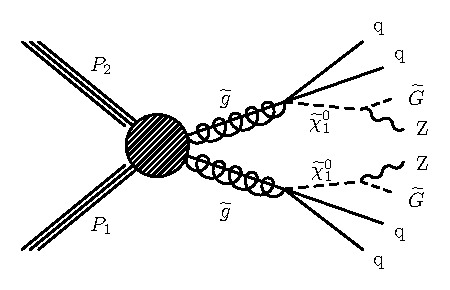
\includegraphics[width=.5\textwidth]{figures/diagrams/T5ZZ.pdf}
    \caption[The Feynman diagram for the additional term added to The Standard Model lagrangian to produce the simplified supersymmetric model used to interpret this in analysis in the context of ``strong SUSY".]{The Feynman diagram for the additional term added to The Standard Model lagrangian to produce the simplified supersymmetric model used to interpret this in analysis in the context of ``strong SUSY". In this model of GSMB, the gravitino is the LSP with an assumed mass of 1 GeV. Two gluinos are produced in the collision which decay to neutral electroweak superpartners that couple to the Z boson. Because the model assumes the production of gluinos, large amounts of hadronic activity is expected.}
    \label{fig:feynman_str}
  \end{figure}

  \begin{figure}
    \begin{center}
      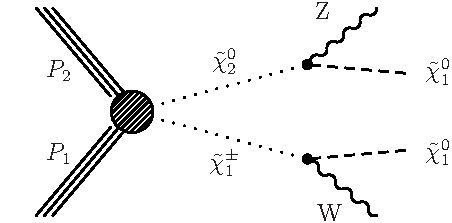
\includegraphics[width=0.3\textwidth]{figures/diagrams/TChiWZ.pdf} 
      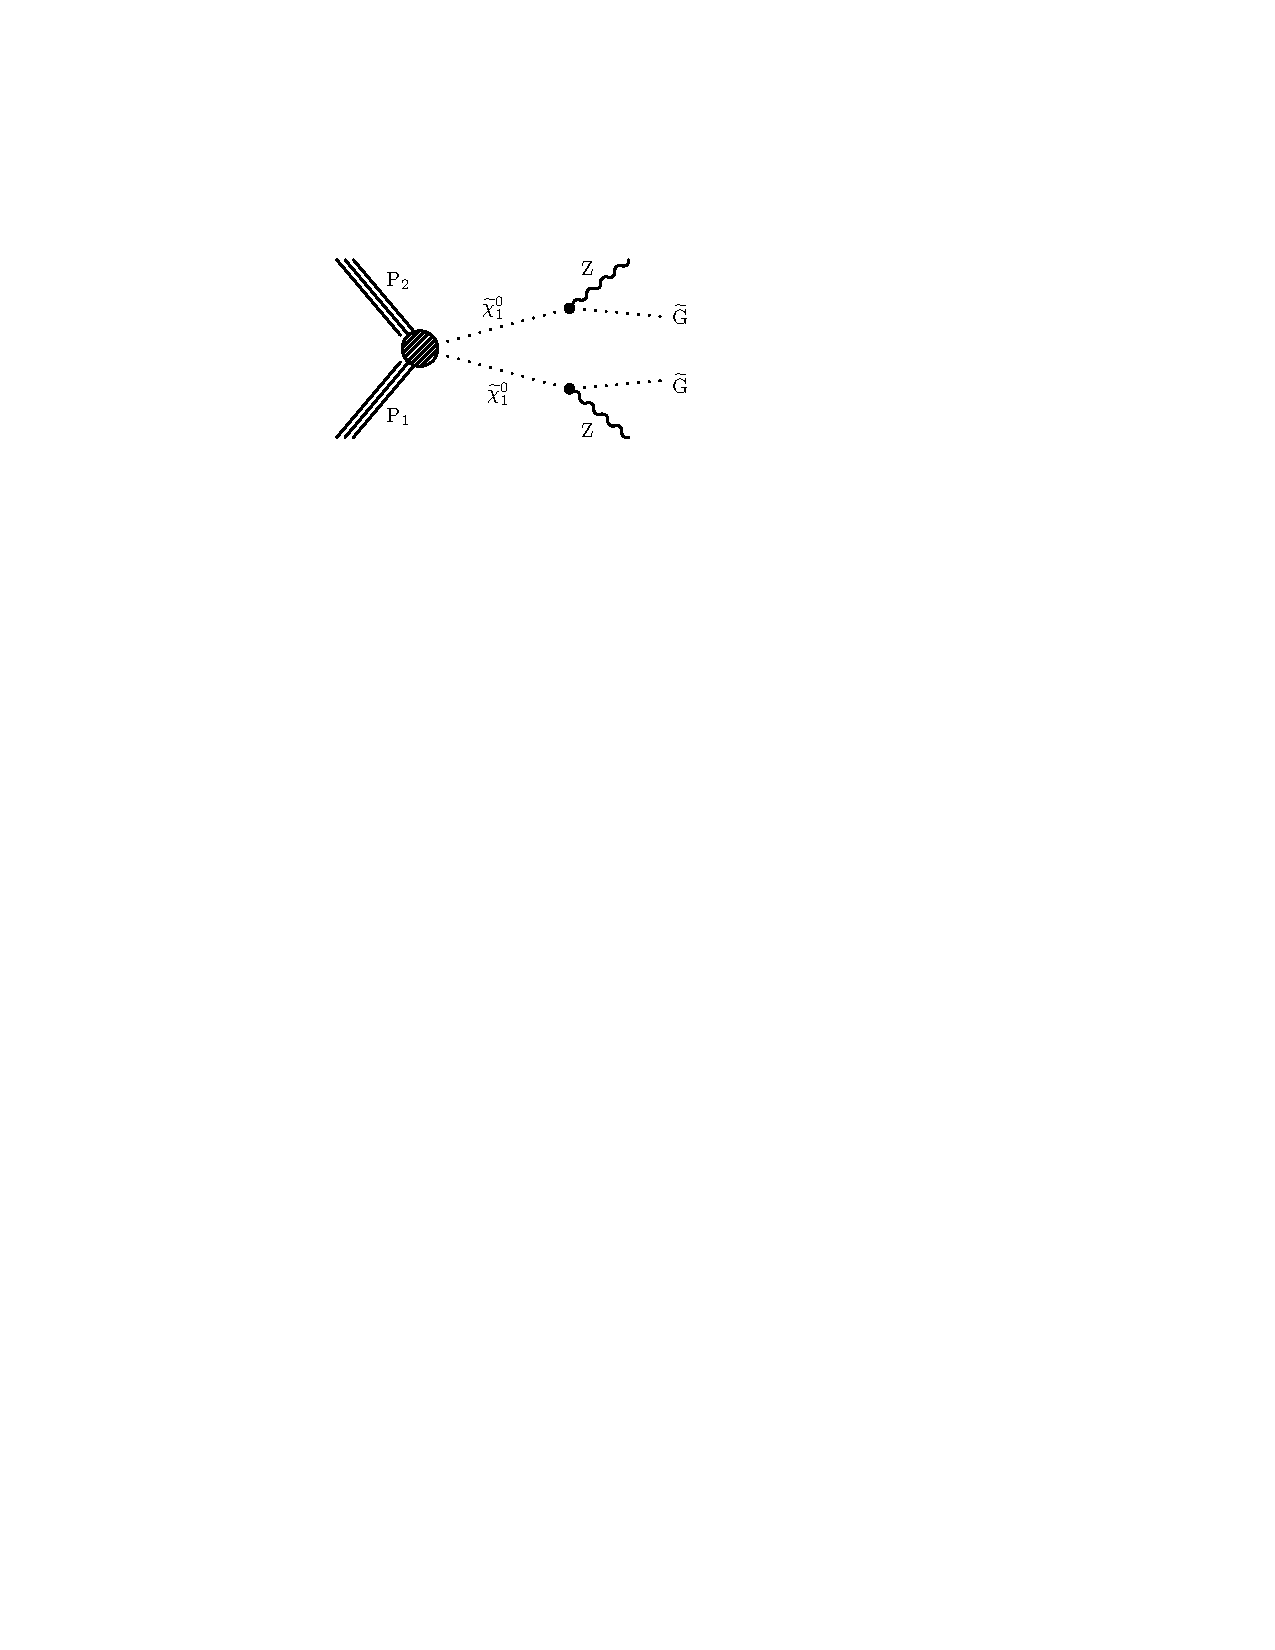
\includegraphics[width=0.3\textwidth]{figures/diagrams/TChiZZ.pdf} 
      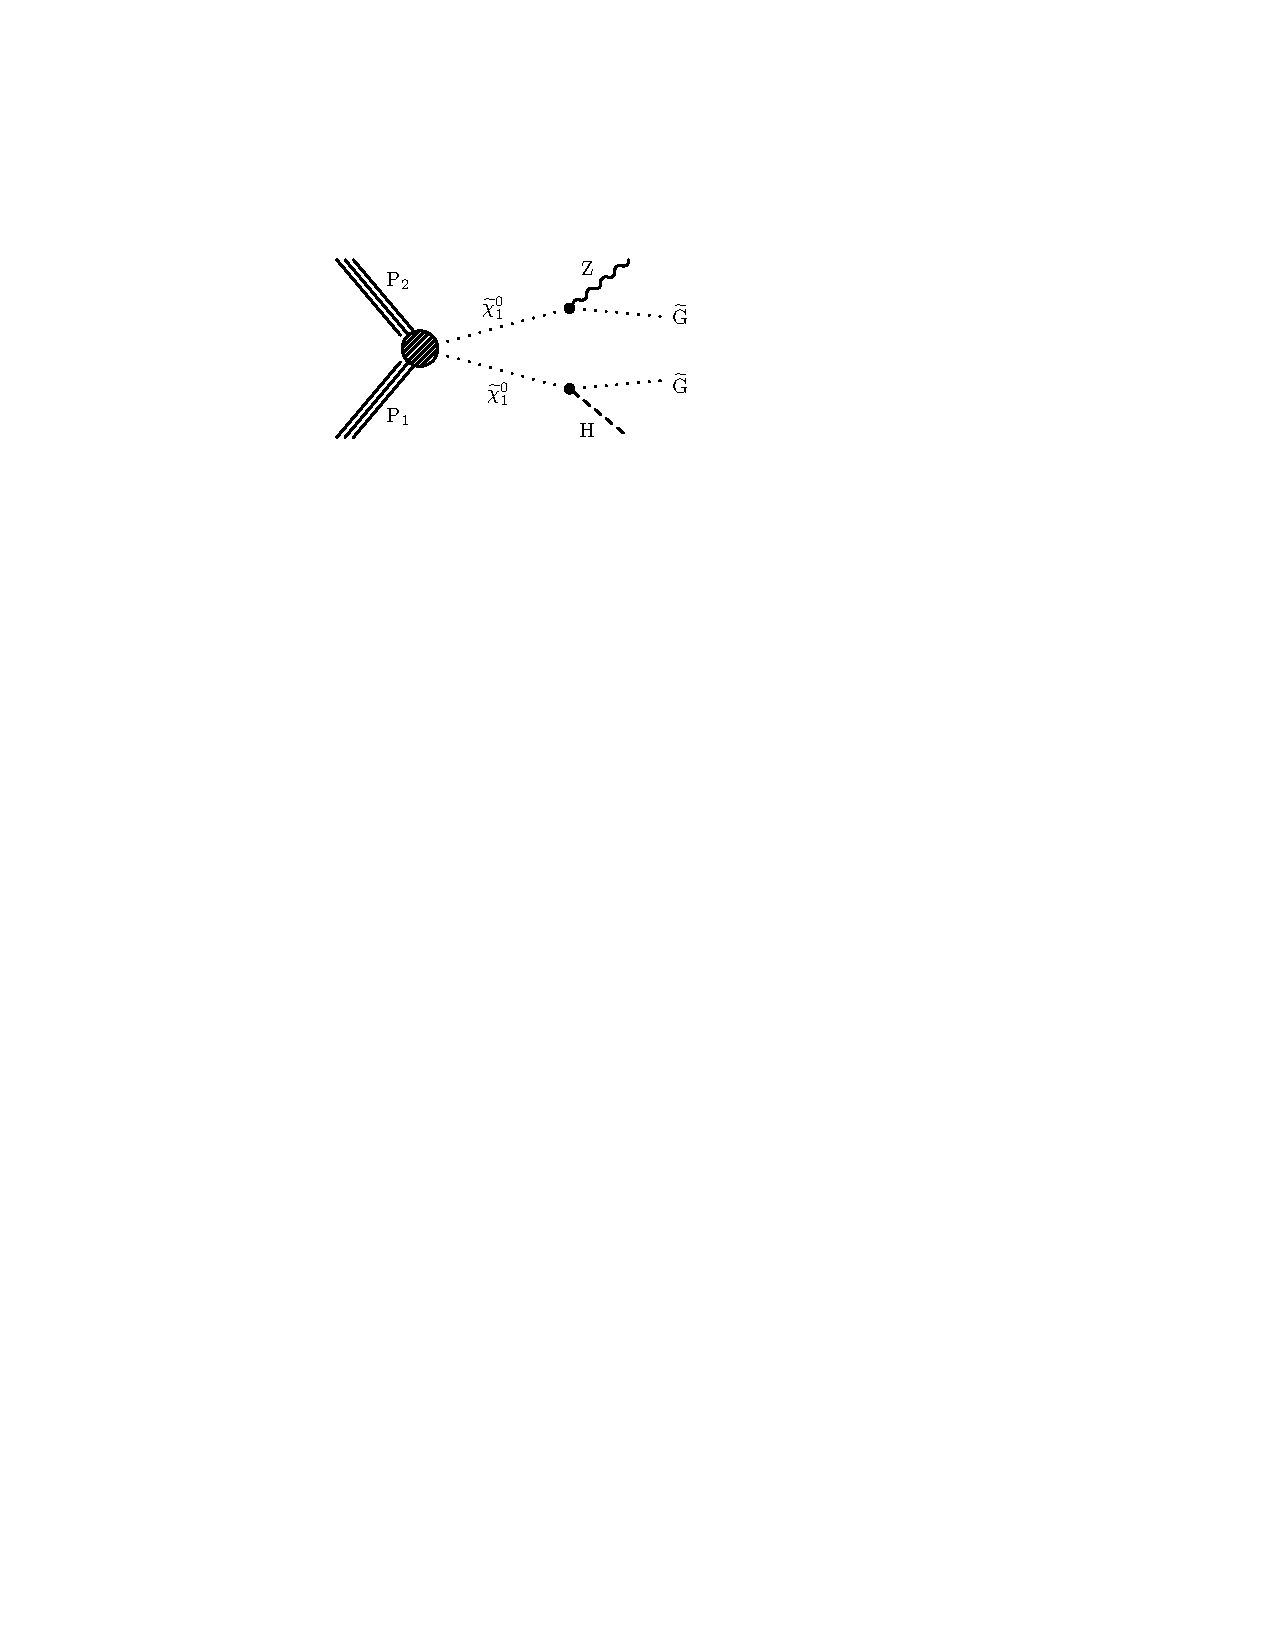
\includegraphics[width=0.3\textwidth]{figures/diagrams/TChiHZ.pdf} 
    \end{center}
    \caption{
      \label{fig:feynman_ewk} The Feynman diagrams for the electroweak SUSY models. In each diagram, electroweak superpartners are created in the collision and decay to either electroweak or Higgs bosons. The right two models again represent GMSB with a gravitino that is assigned a mass of 1 GeV.
    }
  \end{figure}

  \clearpage

\section{Analysis Strategy}

  \subsection{Background Considerations} \label{sec:background_considerations}

    \subsubsection{Leptonic Final States} \label{sec:leptonic_final_states}
      The Z boson can decay to any fermion. In theory, one could perform this analysis in an all hadronic final state, which might seem advantageous as the Z will decay to hadrons approximately 10 times as often as it will decay to light leptons.\cite{PDG} However, there are several reasons leptonic final states are highly advantageous.

      In hadron colliders, the most common types of final states are those with only hadronic activity, as can be seen in figure \ref{fig:lhc_decay_modes}; leptonic final states provide a much cleaner population in which to search for Z bosons. Additionally, as referenced in \ref{sec:electron_measurement_pipeline}, \ref{sec:muon_measurement_pipeline}, and \ref{sec:MET_reco}, the fidelity of energy measurements for the light leptons is much better than for jets at CMS. This provides great advantage for background discrimination; leptons from Z boson decays will tend to have a very specific dilepton mass, a quantity reconstructed from the momentum measurements.

      The decays of the Z produce two opposite sign, same flavor fermions. A further benefit of the leptonic channel is that flavor and charge identification is fairly easy for the light leptons but nearly impossible to identify for jets at the current state of the art (for instance, one can not say with high confidence that a jet was produced by a positively charged charm quark).

      Therefore, even though the branching ratio to light leptons from Z bosons is lower than the branching ratio to hadronic final states, the better energy resolution, lower background rates, and flavor identification make the leptonic final states far more powerful.

    \subsubsection{Background Sources}
      When using the leptonic final states, there are essentially two other background sources of leptons we must consider, these are $\gamma$ and W decays. Due to the high mass of the Z boson, any $\gamma \to \ell^\pm \ell^\mp$ events can easily be vetoed since these events should have dilepton mass peaking at 0 GeV. 

      The W boson will decay into leptons only with their complimentary neutrino, this means that in order to select a pair of opposite charge and same flavor charged light leptons, there must be at least two W bosons in the event. Because the decays of the W will be independent, there is only a 50\% chance that the two leptons will have the same flavor. As will be discussed later, this makes the background prediction for these types of events straightforward as events with two different flavor leptons can be used to model essentially any kinematical distribution.

      It turns out the most common source of W bosons is through the production of two top quarks which decay to a bottom quark and a W boson. To reject these events, we will use the MT2 variable, described in sec \ref{sec:MT2}. Further, the dilepton mass in $t\bar{t}$ events will be distributed essentially flatly across the Z mass window. The overall dilepton mass distribution will be a falling distribution with a small bump for the Z Boson. 

      Finally, due to the instability of the $\tau$ lepton, we neglect this channel from the search. $\tau$ leptons are much harder to identify than the light leptons, and further they can decay to light leptons in a flavor symmetric manner, so are predicted by that background channel's prediction method.

    \subsubsection{Hadronic Activity Requirements}
      As mentioned above, the major production mode of opposite sign dilepton pairs with dilepton mass near 91 GeV is from Drell-Yan production of Z bosons. The diagram for this type of process is shown in fig. \ref{fig:DY-diagram}. As can be seen in the figure, the leading order diagram for this process has no free quarks or gluons. That there are no free colored particles means that the vast majority of these events will likewise come without any jets. 

      \begin{figure}[h!]
        \centering
        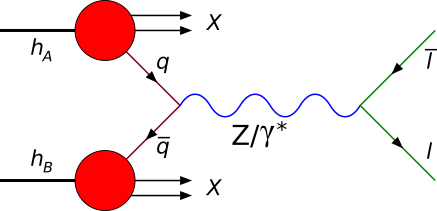
\includegraphics[width=.5\textwidth]{figures/Drell-Yan_feynman_edit.png}
        \caption{A diagram showing the Drell-Yan process. A quark and an anti-quark annihilate into an off-shell $\gamma$ or Z boson, which in turn decays to a pair of opposite-charge same-flavor leptons.}
        \label{fig:DY-diagram}
      \end{figure}

      Higher order diagrams with ISR or FSR take a cross-section production hit of roughly 1/5 due to the additional factor of the QCD coupling, $\alpha_s$, in the phase space integral. This means that we can suppress the DY background by a factor of almost 100 by requiring at least 2 jets in an event. This requirement is adopted in all search regions to keep our Drell-Yan background count low. Further, the background prediction for 0 or 1 jet events would require a completely different methodology due to different sources of \MET in high jet multiplicity final states. Therefore, this analysis limits itself to final states with at least 2 jets. 

      \begin{figure}[h!]
        \centering
        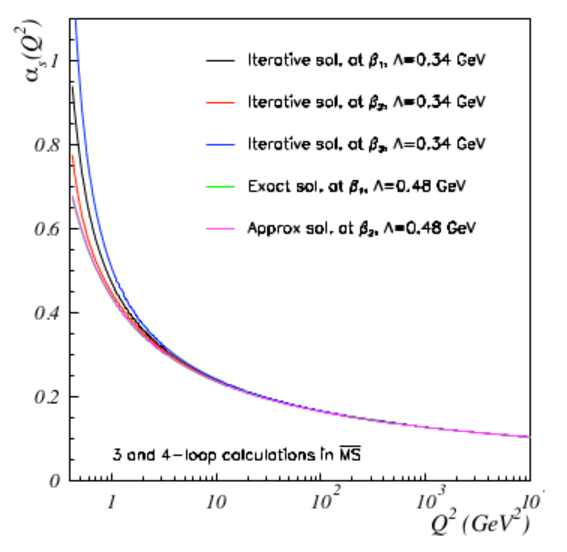
\includegraphics[width=.5\textwidth]{figures/QCD_Coupling_Running.pdf}
        \caption[The QCD coupling constant computed to different orders and different cutoff scales.]{The QCD coupling constant computed to different orders and different cutoff scales. The production of the Z boson is much more likely at center of mass energy near the mass of the Z. This means that $\alpha_s$ is between $\frac{1}{5}$ and $\frac{1}{10}$, which can be viewed as the zeroth order multiplicative correction to the DY with a single ISR or FSR jet cross section} 
        \label{fig:alpha_s_running}
      \end{figure}

      In addition, the strong SUSY model shown in fig. \ref{fig:feynman_str} anticipates lots of hadronic activity. Therefore, in the strong search regions, we also bin in the number of jets\footnote{This has the added benefit of creating search regions which are dominated by only one of the two dominant backgrounds, $t\bar{t}$ and Drell-Yan.} and require considerable hadronic activity by selecting events with $H_T$\footnote{$H_T$ is the scalar sum of transverse energy for all jets in an event, above certain thresholds.} above 200 or 500 GeV for the regions with and without b-tags respectively. This further rejects Drell-Yan events.


    \subsubsection{\MET Binning}

      Dark particles are expected to leave no signature in the detector except transverse momentum imbalance. In order to get maximal sensitivity to the different mass points for the SUSY models, we bin the search regions in \MET.

    \subsubsection{B-Tagging} \label{sec:b-tagging_selection}
      We bin search regions in number of b-tags, which are outlined in detail in sec \ref{sec:b-tagging}. For the region targeting the HZ model, this is because the Higgs primarily decays to a pair of b-quarks. For the VZ model, we require there be no b-tags as it suppresses the $t\bar{t}$ background. For the strong search regions, we separate regions based on whether they have any b-tags, this because it causes the background composition to change dramatically; in regions with a b-tag, the dominant background will be $t\bar{t}$, whereas in regions without any b-tags the dominant background will be Z+jets. In turn, this allows us to use a slightly more aggressive MT2 cut in regions with a b-tag.

    \subsubsection{MT2} \label{sec:MT2}
      The MT2 variable is defined as

      \[
      \text{MT2} = \min \limits_{\text{\MET splittings}} \left[ \max \left\{ \MT(p_1, \slashed{p}_1), \MT(p_2, \slashed{p}_2) \right\} \right]
      \]

      where $\slashed{p}_1$ and $\slashed{p}_2$ are decompositions of the \MET vector, and M$_{\text{T}}$ is the transverse mass. 

      \begin{figure}[h!]
        \centering
        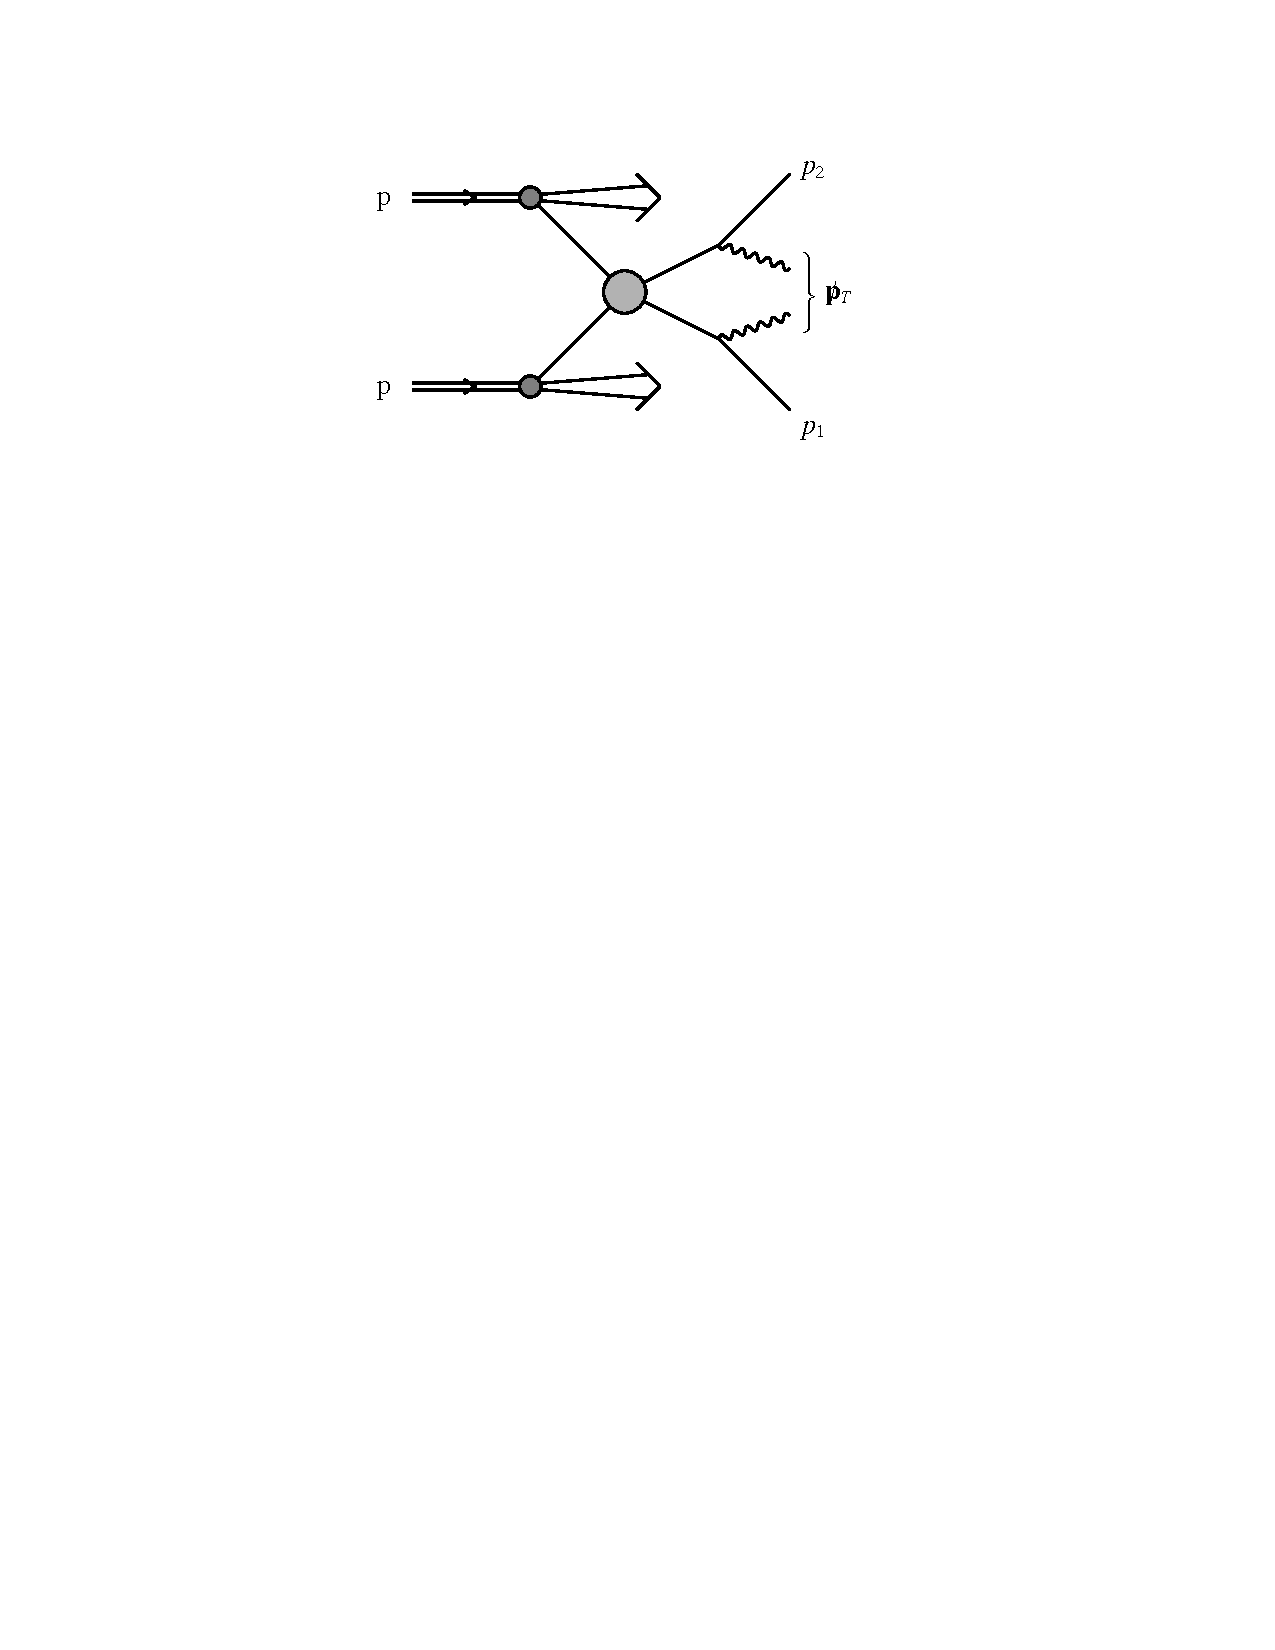
\includegraphics[width=.5\textwidth]{figures/mt2_diagram.pdf}
        \caption{The canonical picture of a decay with an MT2 endpoint, taken from the original paper\cite{mt2_paper}. }
        \label{fig:MT2_feynman_diagram}
      \end{figure}

      When a pair of W bosons each decay into a lepton and a neutrino, this value should not be able to be larger than the mass of the W boson. We can see this is true because for the correct splitting of the \MET vector into the momenta of the two neutrinos, the \MT for each lepton is bounded by the W mass. Therefore by summing over all possibilities, we will ensure the outer minimum will select at most the mass of the W (there is no lower limit besides 0). 

      However, in the case of an arbitrary decay, for instance in DY or in signal models with dark matter, there is no need for this value to be smaller than the mass of the W and generally higher values will be found. Therefore, we can use this quantity as a handle for rejecting events where the leptons come from two W bosons. We require in our strong search regions that MT2 be at least 80 GeV, just about the mass of the W boson. This mainly rejects the $t\bar{t}$ background. 

    \subsubsection{MT2b}

      \begin{figure}[h!]
        \centering
        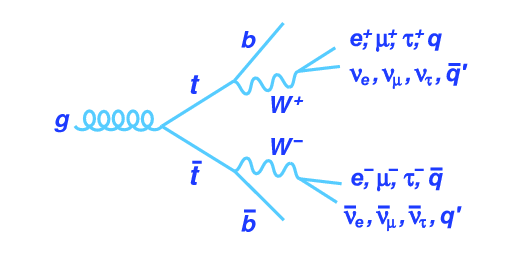
\includegraphics[width=.5\textwidth]{figures/ttbar_diagram.png}
        \caption{Diagram of $t\bar{t}$ production. An MT2-like endpoint can be found at the top mass if the lepton and b-quark momentum vectors are added so that choosing the \MET splitting that corresponds to the actual neutrino momenta will recover the transverse 4-vector of the top at the root of the decay. Figure taken from \cite{TTBar_figure}.}
        \label{fig:ttbar_diagram}
      \end{figure}

      Another variable used in this analysis is MT2b, or sometimes MT2($\ell b \ell b$), which can only be computed in events with 2 jets that are b-tagged. MT2 can be computed for any pair of 4-vectors along with a \MET vector. In the case of $t\bar{t}$ decays, shown in figure \ref{fig:ttbar_diagram}, one can see that by summing the 4-vectors for the lepton and b-quark, an MT2 end point should be found at the top mass, so long as the correct b-quark can be associated with the correct lepton. 

      The same power of MT2 to reject semi-invisibly decaying pair produced particles can be used to reject $t\bar{t}$ events in a population with 2 b-jets by trying the two different combinations of b-jet/lepton pairing and selecting the minimum value out of those two. Again, in the case of $t\bar{t}$ decay, MT2b defined in this way will have the mass of the top quark as one of the possible combinations, whilst there is no such requirement for a general process. MT2b is used only in the electroweak HZ region.

\section{Object Selection} \label{sec:object_selection}


  After the particle flow algorithm identifies lepton, jet, and photon candidates, and before events can be classified as belonging to the various search, control, and closure regions, an additional set of selections are applied in order to further purify the analysis object collection. The purpose of this section is to define these selections.

  \subsection{Lepton ID} \label{sec:lepton_id}
    There are essentially two ways to get ``fake" leptons in the particle-flow lepton population:

    \begin{enumerate}
      \item A set of calorimeter and tracker hits from hadronic activity mimics the geometry expected by an lepton closely enough that a lepton is reconstructed from what should be called, for instance, a charged hadron and a photon.
      \item A colored particle, normally a charm or bottom quark, emits an electroweak boson that decays into a real lepton. In physics parlance, this is called \emph{non-prompt} lepton, as it is a secondary decay (\emph{prompt} meaning created at the primary vertex).
    \end{enumerate}

    Although (2) is a ``real" lepton in the colloquial sense, they are background objects that contaminate the lepton population in the context of most analyses, which aim to study particles produced directly in proton-proton interactions. To guard against these fake leptons, an additional set of cuts, called an ID, are required to be passed by each candidate before it is considered a ``good" lepton.

    In this analysis, we identify two ``working points" for leptons, tight and loose. These categories are defined based the lepton flavor and a set of cuts described below. Any lepton which passes the criteria to be classified as tight would necessarily pass the criteria to be classified as loose.

  \subsection{Lepton Isolation}
    In addition to the ID, isolation requirements are also necessary for leptons to be added to the analysis selection. In this analysis we use the variable miniRelIso, which is defined as the energy inside a variable size cone, determined by the lepton candidates \pt, about the lepton divided by the leptons \pt. The cone size is set by \pt in the following manner (units in \GeV):

    \[   
      \Delta R = 
      \begin{cases}
        0.2                & \pt < 50  \\
        \frac{10}{\pt}     & 50 \le \pt < 200 \\
        0.05               & \pt \ge 200 \\
      \end{cases}.
    \]

    The miniRelIso variable is then defined as the energy of all particle flow candidates inside the cone of size $\Delta R$ with effective area\footnote{See sec \ref{sec:jets}} corrections applied divided by the \pt of the lepton.

    \[
      \text{miniRelIso} = \frac{\text{E}_\text{cone}}{\pt}.
    \]

  \subsection{Electron ID and Isolation} \label{sec:electron_id_and_isolation}

    The electron candidates are required to pass the following cuts in addition to the particle flow identification:

    \begin{table}[!h]
      \begin{center}
      \caption[Requirements for electron identification in addition to particle flow.]{\label{table:electrons} Requirements for electron identification in addition to particle flow. $d_{0}$ and $d_{z}$ represent the closest distance of the lepton track to the primary vertex in the x-y plane and along the z axis respectively. The SIP3D variable is the impact parameter significance, $\frac{\sigma_\text{ip}}{\text{ip}}$, where the impact parameter is the closest distance of the lepton track to the primary vertex in 3 dimensions. The conversion veto attempts to reject photon conversions into electrons.\cite[sec. 5.3]{cms_electrons}}
        \begin{tabular}{l|c}
          \hline
          Cut variable                  & Requirement   \\
          \hline
          \pt\                           & $>10$ GeV    \\ 
          $d_{0}$ (w.r.t. 1st good PV)   & $<0.05$ cm   \\
          $d_{z}$ (w.r.t. 1st good PV)   & $<0.1$  cm   \\
          miniRelIso                     & $<0.10$      \\
          abs(SIP3D)                     & $< 8$        \\
          maxLostHits                    & $==$ 0       \\
          Conversion Veto                & must pass    \\
          Spring 2016 POG MVA            & see below    \\
          miniRelIso                     & $<0.10$      \\
          \hline
        \end{tabular}
      \end{center}
    \end{table}

    The tight and loose criteria for electrons is based entirely on the MVA output. The POG MVA is a boosted decision tree (BDT)\footnote{A boosted decision tree is a sort of classifier that assigns a real number to a well-formed tuple of data. The algorithm tries to construct a map such that the number output for tuples in the same category are close to each other, then that number can be used discriminate between categories. Technical details are beyond the scope of this thesis, but a good review can be found \cite{boosting}. In the case of the electron ID MVA, the categories are real or fake and the numbers lie between -1 and 1.} prepared by the CMS EGamma Physics Object Group (POG). The BDT is trained on simulated Z$\to e^+ e^-$ events where electrons are considered to be real if the candidate can be matched to an electron emitted from the Z, and fake otherwise. An additional validation sample of mostly real electrons in data is constructed from $e^+ e^-$ events where the dilepton mass is within 7.5 GeV of the Z pole mass, $\abs{M_{ll} - M_Z} < 7.5$ GeV, and each lepton is required to be isolated such that the energy in a cone around the electron must be less than 10\% of the total energy in the cone (including the electron). A sample of mostly fake leptons in data is constructed by requiring a third lepton candidate in these events which has inverted isolation criteria and the additional requirement that the \MET in the event is less than 25 GeV to suppress WZ events. 

    Distributions of various kinematical quantities are constructed from simulation and data that have reason to discriminate between real and fake electrons, for instance the spread of the calorimeter hits in $\eta$. Some of these distributions are shown in figure \ref{fig:electron_mva_discriminating_vars}. The MVA is trained on the simulated events then checked against the data samples described above for consistency. Finally electrons in the barrel region and endcap regions are partitioned and each set is used to train an MVA specifically targeting the detector subsystems there \cite{Electron_reco}. 

    \begin{figure}[!h]
      \centering
      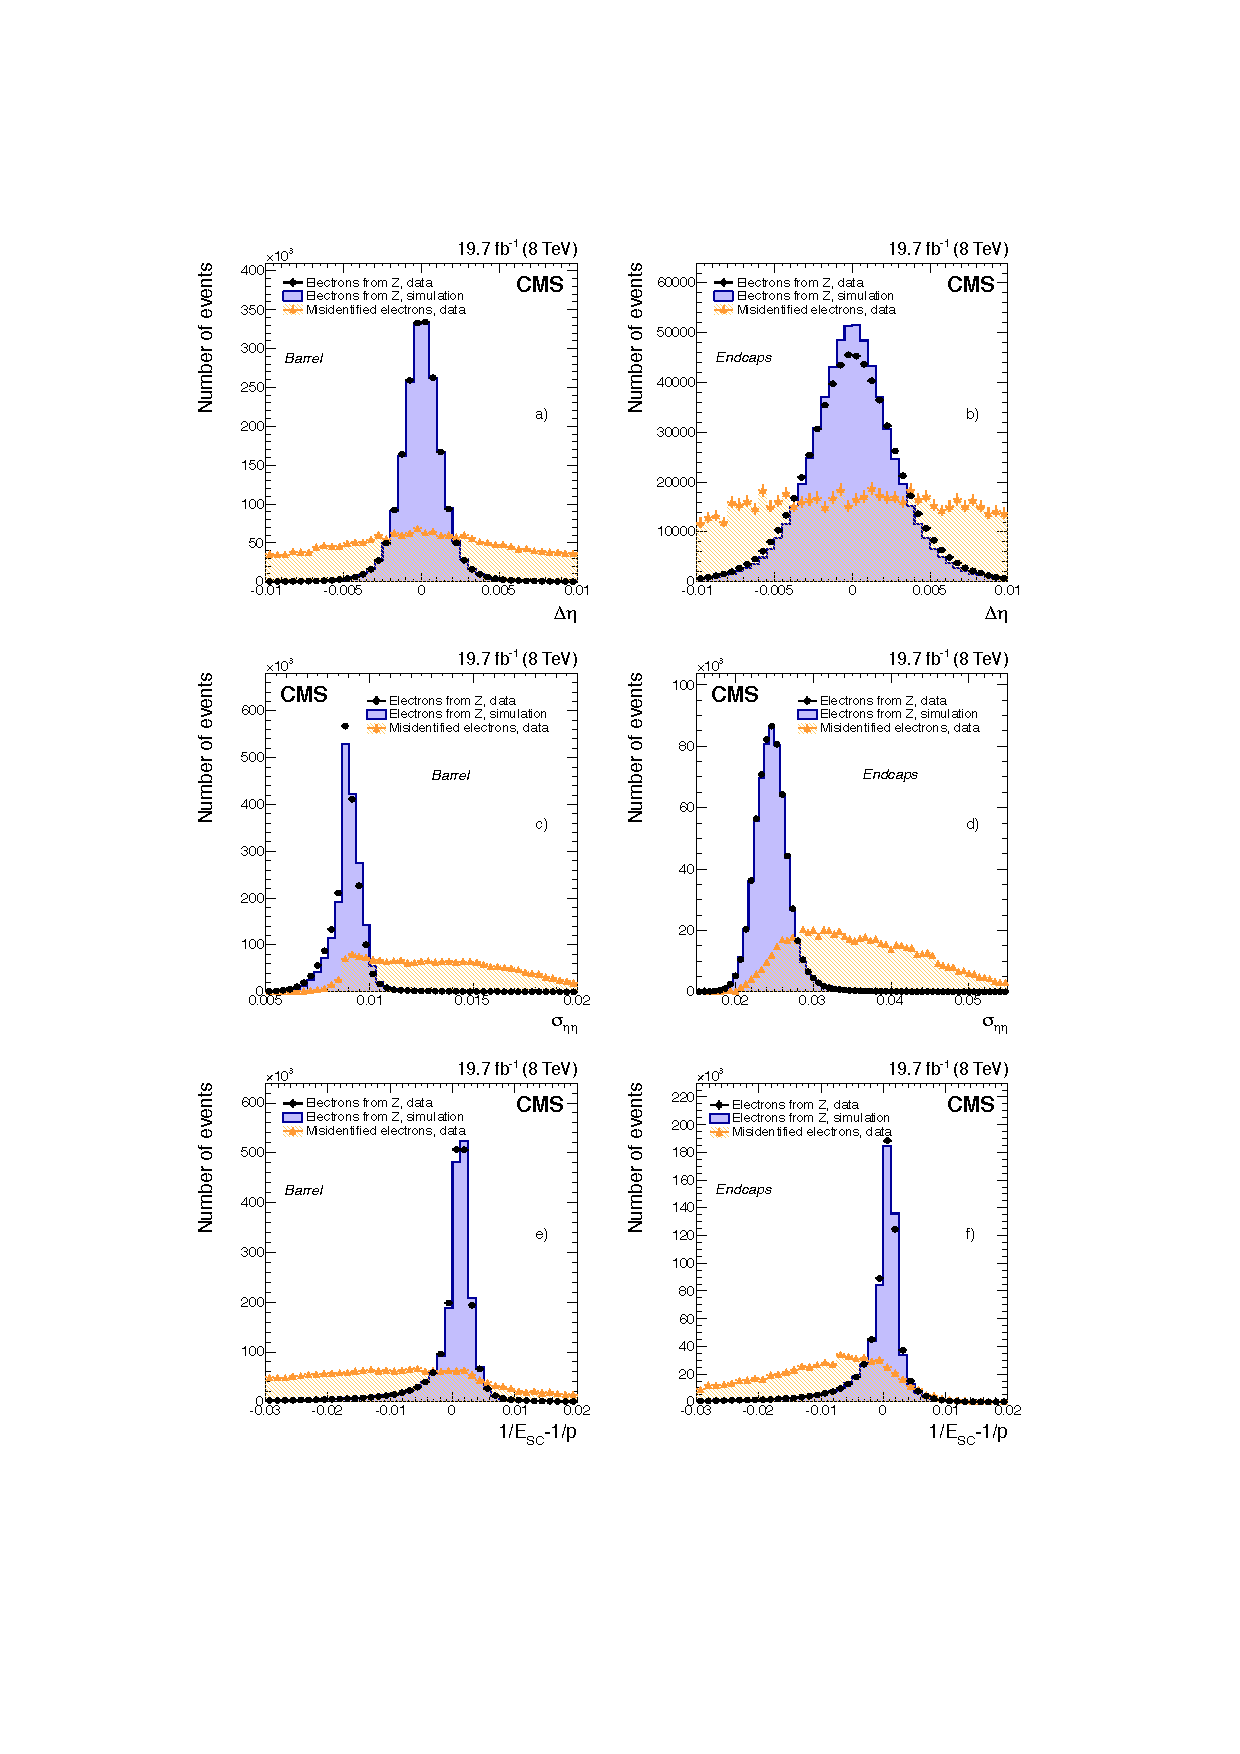
\includegraphics[width=.8\textwidth]{figures/electron_mva_discriminating_distributions.pdf}
      \caption[Some distributions used in the electron MVA that help discriminate between real (prompt) and fake (non-prompt) electrons.]{Some distributions used in the electron MVA that help discriminate between real (prompt) and fake (non-prompt) electrons. Simulation provides a guaranteed way to tag electrons as prompt or not-prompt, and so is used to train the MVA. However, it is important that data and simulation agree in these variables. $\Delta \eta$ and $\sigma_{\eta\eta}$ are variables that characterize the spread of detector hits associated with the electron in the $\eta$ direction. $E_\text{SC}$ is all the energy deposited into the ECAL which is associated to the electron, and $p$ is the electron's momentum.}
      \label{fig:electron_mva_discriminating_vars}
    \end{figure}

    The working points for electrons based on the MVA output are shown below:

    \begin{table}[!h]
      \begin{center}
        \caption{\label{tab:elId}  Electron identification working points used in this analysis.}
        \begin{tabular}{rl|rl|l|l}
          \hline
          \multicolumn{2}{c|}{pseudorapidity region} & \multicolumn{2}{c|}{momentum [GeV]} & loose WP & tight WP \\ 
          \hline\hline
          $0<~|\eta|$&$<0.8$     &  10 $<$ ~\pt\ &$<$ 15 &  -0.86 & 0.77 \\ 
          $0<~|\eta|$&$<0.8$     &  15 $<$ ~\pt\ &$<$ 25 &  -0.96+$0.10*\frac{\pt-15}{10}$ & 0.52+$0.25*\frac{\pt-15}{10}$ \\ 
          $0<~|\eta|$&$<0.8$     &   ~\pt\ &$>$ 25       &  -0.96 & 0.52 \\ 
          \hline
          $0.8<~|\eta|$&$<1.479$ &  10 $<$ ~\pt\ &$<$ 15 &  -0.85 & 0.56 \\ 
          $0.8<~|\eta|$&$<1.479$ &  15 $<$ ~\pt\ &$<$ 25 &  -0.96+$0.11*\frac{\pt-15}{10}$ & 0.11+$0.45*\frac{\pt-15}{10}$ \\ 
          $0.8<~|\eta|$&$<1.479$ &   ~\pt\ &$>$ 25       &  -0.96 & 0.11 \\ 
          \hline
          $1.479<~|\eta|$&$<2.5$ &  10 $<$ ~\pt\ &$<$ 15 &  -0.81 & 0.48 \\ 
          $1.479<~|\eta|$&$<2.5$ &  15 $<$ ~\pt\ &$<$ 25 &  -0.95+$0.14*\frac{\pt-15}{10}$ & -0.01+$0.49*\frac{\pt-15}{10}$ \\ 
          $1.479<~|\eta|$&$<2.5$ &  ~\pt\ &$>$ 25        &  -0.95 & -0.01 \\ 
          \hline\hline
        \end{tabular}
        
      \end{center}
    \end{table}

    \clearpage

  \subsection{Muon ID and Isolation} \label{sec:muon_id_and_isolation}

    The muon ID is based purely on a cut-based approach, no MVA is used. Again, the selection criteria is based upon the muon POG, which is documented in more detail at ~\cite{muon_POG}. The selection used for the muon ID and isolation are defined below:

    \begin{table}[!h]
      \begin{center}
        \caption[Summary of the muons selection requirements.]{\label{table:muons} Summary of the muons selection requirements. $d_{0}$ and $d_{z}$ represent the closest distance of the lepton track to the primary vertex in the x-y plane and along the z axis respectively. The SIP3D variable is the impact parameter significance, $\frac{\sigma_\text{ip}}{\text{ip}}$, where the impact parameter is the closest distance of the lepton track to the primary vertex in 3 dimensions.}
        \begin{tabular}{l|c|c}
          \hline
          \hline
          \multicolumn{3}{c}{Good Muon Requirements} \\
          \hline
          Quantity   &  Tight Requirement & Loose Requirement \\
          \hline
          Quality Muon                      & Must pass   & Must pass     \\
          Fraction of valid tracker hits    & $>$ 0.8     & $>$ 0.8  \\ 
          \hline
          $d_{0}$ (w.r.t. 1st good PV)   & $<0.05$ cm & $<0.05$ cm \\
          $d_{z}$ (w.r.t. 1st good PV)   & $<0.1$ cm  & $<0.1$ cm  \\
          SIP3D                          & $< 8$      & $< 8$      \\
          miniRelIso                     & $<0.20$    & $<0.40$       \\
          \hline
        \end{tabular}
      \end{center}
    \end{table}

    The criteria to be a ``Quality Muon" is given below:
    \begin{table}[!h]
      \begin{center}
        \caption[Summary of Quality Muon requirements.]{\label{table:muons} Summary of Quality Muon requirements. The segment compatibility is an internal CMS variable which characterizes how well the global muon track matches track segments in the muon system. The global track $\chi^2$ tests the fit of the muon track fits the hits in the tracker and muon system. The $\chi^2_\text{kink}$ represents the probability that the muon was the result of a decay in flight.}
        \begin{tabular}{l|c}
          \hline
          \hline
          \multicolumn{2}{c}{Quality Muon Requirements} \\
          \hline
          Quantity   &  Requirement \\
          \hline
          Segment compatibility             &$>$ 0.451 \\
          \hline
          \emph{or} & \\
          \hline
          Normalized global-track $\chi^2$  & $<$ 3    \\
          Tracker-Standalone position match & $<$ 12   \\
          Kink finder                       & $<$ 20   \\
          Segment compatibility             & $>$ 0.303 \\
          \hline
          \hline
        \end{tabular}
      \end{center}
    \end{table}

  \newpage

  \subsection{Photon Selection} \label{sec:photon_selection}

    Photons are used in this analysis as part of the Z+Hadronic background prediction. The details of this prediction are in \ref{sec:z_+_hadronic}. The bulk of these selections are in order to ensure there is no inefficiency for the trigger for $\gamma +$jets events.

    \begin{itemize}
      \item \pt $ > 25$ GeV
      \item $|\eta| < 2.4$
      \item No matching pixel track (pixel veto)
      \item There must be a jet candidate of \pt $ >$ 10 GeV matched to the photon within $\DR < 0.3$. 
      The matched jet is required to have a neutral electromagnetic energy fraction of at least 70\%.

      \item We reject photons which have an electron of at least \pt $>$ 10 GeV within $\DR < 0.2$
      in order to reject conversions from electrons from W decays which are accompanied by real \MET.

      \item We reject photons which are aligned with the \MET to within 0.4 radians in phi.
      \item To ensure full efficiency with respect to the isolated photon triggers used, we apply the following additional cuts:
      \begin{itemize}
        \item ratio of the energy of the energy of the photon's 3X3 supercluster to the photons 5X5 supercluster (R9) $>$ 0.92
        \item $\frac{H}{E} < 0.2$ %\fixme{is this the HLT H/E or still offline?}
        \item hollow track isolation $<$ 3 GeV
        \item photons with $|\eta| < 1.4$ have ECAL pfcluster iso $<$ 3 GeV + \pt ($\gamma$) * 0.0053
        \item photons with $|\eta| < 1.4$ have HCAL pfcluster iso $<$ 7 GeV + \pt ($\gamma$) * 0.014
        \item photons with $|\eta| > 1.6$ have ECAL pfcluster iso $<$ 3 GeV + \pt ($\gamma$) * 0.0034
        \item photons with $|\eta| > 1.6$ have HCAL pfcluster iso $<$ 7 GeV + \pt ($\gamma$) * 0.0139
      \end{itemize}
    \end{itemize}

    %\todo{Photon ID: https://github.com/cmstas/CORE/blob/master/OSSelections.cc#L360-L370}
    %\todo{Loose Selection: https://github.com/cmstas/CORE/blob/master/PhotonSelections.cc#L308-L342}
    %\todo{Template Photon: https://github.com/cmstas/CORE/blob/master/PhotonSelections.cc#L186-L192}
    %\todo{Trigger Emulation: https://github.com/cmstas/CORE/blob/master/PhotonSelections.cc#L420-L444}

  \subsection{Jet Selection} \label{sec:jet_selection}

  Jets are selected from the particle flow selection and are refined via ``charged hadron subtraction" and the Summer16\_23Sep2016V3 ``jet energy corrections" described in \ref{sec:jets}. In this analysis, we distinguish between jets and ``b-tagged jets." B-tagging is described in \ref{sec:b-tagging}, but it comes down to a numerical quantity assigned to each jet called its \emph{b-tag csv value}. If the csv value is large enough, a jet is considered likely to have been seeded by a bottom quark. 

      \begin{table}[!h]
      \begin{center}
        \caption[Summary Of Good Jet Requirements.]{\label{table:muons} Summary Of Good Jet Requirements. The photon veto and cut on the fraction of energy found in the ECAL without an associated track (neutral EM fraction) attempts to veto jets that are truly photons. The lepton veto and cut on the fraction of energy from the ECAL with an associated track (charged hadron and charged EM fraction) attempt to veto jets that are truly leptons. The cuts on neutral hadron fraction and number of constituents ensure the jets are really sprays of hadronic particles. The cut on \pt attempts to remove jets from pileup collisions from consideration.}
        \begin{tabular}{l|c|c}
          \hline
          \hline
          \multicolumn{3}{c}{Jet Selections} \\
          \hline
          \hline
          Quantity                  & \multicolumn{2}{c}{ Cut Value } \\
          \hline
          $\abs{\eta}$              & \multicolumn{2}{c}{$< 2.4$}   \\
          Lepton Veto               & \multicolumn{2}{c}{Not within $\abs{\DR} < 0.4$ of a tight lepton} \\
          Photon Veto               & \multicolumn{2}{c}{Not within $\abs{\DR} < 0.4$ of a good photon } \\
          Neutral Hadron Fraction   & \multicolumn{2}{c}{ $< 0.99$} \\
          Neutral EM fraction       & \multicolumn{2}{c}{ $< 0.99$} \\
          Charged hadron fraction   & \multicolumn{2}{c}{ $> 0   $} \\
          Charged multiplicity      & \multicolumn{2}{c}{ $> 0   $} \\
          Charged EM fraction       & \multicolumn{2}{c}{ $< .99 $} \\
          Number of constituents    & \multicolumn{2}{c}{ $> 1   $} \\
          \hline
          \hline
          Quantity                  &  Jet Requirement & B-tagged Jet Requirement\\
          \hline
          \pt                       & $> 35\; \GeV $     & $> 25\; \GeV$   \\
          B-tag CSV                 & None             & $> 0.8484$    \\
          \hline
          \hline
        \end{tabular}
      \end{center}
    \end{table}

  \subsection{Isolated Tracks} \label{sec:isolated_tracks}
  In addition to vetoing events which have extra loose leptons, a typically more inclusive veto is applied to kill events which might have an extra prompt lepton based on the identification of an isolated charged object. 

  To distinguish these types of objects, we introduce the notion of ``track isolation," defined as the total energy of all the particle flow charged candidates that trace back to within $\abs{dz} < 0.1$ cm of the primary vertex within a cone of $\abs{\DR} <0.3$ about the lepton.\footnote{Notice that the miniRelIso we defined above was defined as a relative isolation, the energy in a cone divided by the \pt of the object in question, track isolation as defined here has units of energy.}

  There are two types of isolated tracks, those that identified by particle flow as charged hadron candidates, and those that are identified by particle flow as electron or muon candidates. The criteria on top of the particle flow identification for these two sources are listed in the tables below:

  \begin{table}[!h]
      \begin{center}
        \caption{\label{table:muons} Summary Of Isolated Track Requirements.}
        \begin{tabular}{l|c|c}
          \hline
          \hline
          \multicolumn{3}{c}{Isolated Track Selections} \\
          \hline
          \hline
          Quantity                  &  Charged Hadronic Requirement & Light Lepton Requirement\\
          \hline
          \pt                       & $> 10\; \GeV $                & $> 5\; \GeV$           \\
          Vertex Association\footnote{PVTight means the particle was closer to the primary vertex than any other reconstructed vertex. PVUsedInFit means the particle was used to define the primary vertex.}     & PVTight or PVUsedInFit  & PVTight or PVUsedInFit \\ 
          Track Isolation           & $<8\; \GeV$                   & $<8\; \GeV$             \\
          Track Isolation / \pt     & $<0.2$                        & $<0.1$                  \\
          $\abs{dz}$                & $< 0.1$ cm                    & $< 0.1$ cm              \\
          \hline
          \hline
        \end{tabular}
      \end{center}
    \end{table}


\section{Event Selection} \label{sec:event_selection}

  The selection of events can be broken into several stages. Though each of these regions will be expanded upon in the following sections, in broad strokes there 4 separate final states used to accomplish this analysis. These final states define the signal regions and 3 control regions used to conduct this search:

  \begin{description}
    \bitem{Search Regions (SR)} Events with two opposite charge and same flavor light leptons build our search regions, we have either a $e^+e^-$ or a $\mu^+ \mu^-$ pair in each event.
    \bitem{Flavor Symmetric Control Regions} Events with two opposite charge and different flavor light leptons build our flavor symmetric control region, we have either a $e^+\mu^-$ or a $\mu^+ e^-$ pair in each event. This region is used to predict the flavor symmetric background.
    \bitem{$\gamma$+Jets Control Region} Events with a single photon are used to construct the $\gamma$+jets control region used for the Z+jets background prediction. 
    \bitem{EWK Contamination Closure Region} Events with a photon and muon are used to check the modeling of the ``EWK contamination" in the \MET Templates prediction, described in section \ref{sec:ewk_subtraction}.
  \end{description}

  The CMS datasets which seed these events are described in \ref{sec:datasets}.
  
  \subsection{Dilepton Selection} \label{sec:dilepton_selection}

    The following are the requirements for events with two light leptons, i.e. for the search regions and for the flavor symmetric control regions.  

    Light lepton candidates are tagged by the particle flow algorithm described in section \ref{sec:particle_flow}. In addition to the list below, leptons must also pass preselection ID and isolation requirements which differ depending on their flavor, but are described in \ref{sec:electron_id_and_isolation} and \ref{sec:muon_id_and_isolation} above.

    \begin{itemize}
      \item The (sub)leading lepton in each event must have at least (20) 25 GeV of transverse momentum. These points were selected so that the event would be in the "trigger turn-on" described in \ref{sec:event_triggering}.
      \item The pseudorapidity for each lepton must be within the inner tracker's fiducial area, namely $\left|\eta\right| < 2.4$
      \item No lepton should be in the ``dead zone", described in section \ref{sec:inner_tracker}, this is the range $1.4 < \left|\eta\right| < 1.6$
      \item For the search region, events must have exactly one pair of opposite charge same flavor (OCSF) light leptons, for the flavor symmetric control region events must have exactly one pair of opposite charge and different flavor (OCDF) light leptons.
      \item The mass constructed out of the sum of lepton vectors (dilepton mass) must be between 86 and 96 GeV.
      \item The transverse momentum of the dilepton system must be at least 25 GeV. This is in order to ensure parity with the $\gamma$ selections used in the Z+hadronic background prediction.
    \end{itemize}

  \subsection{Event Vetos} \label{sec:event_vetos}
    Events are typically vetoed\footnote{precise definitions of the regions will be given below} across all search, control, and closure regions if any of the following are true:

    \begin{description}
      \bitem{Isolated Track Veto} Events with an isolated track, defined in \ref{sec:isolated_tracks}.
      \bitem{\MET Filters} Events where any of the ``\MET Filters", described in section \ref{sec:met_filters}, are true.
      \bitem{Jet/\MET alignment} Events where the \MET is aligned with the leading or subleading jet in the $\phi$ direction up to 0.4. Events with $\abs{\Delta \phi(\text{jet}_{1,2},\MET)} < 0.4$ are not accepted. 
    \end{description}

    Dilepton events specifically, those within the SRs and flavor symmetric control regions, are vetoed under the following conditions:

      \begin{description}
        \bitem{Lepton Cone Isolation} The two tight leptons are within a cone of $\Delta R < 0.1$ of each other.
        \bitem{Extra Lepton Veto} There is an additional loose or tighter lepton in the event. In other words, event with three or more loose IDed leptons are vetoed. IDs are defined in \ref{sec:electron_id_and_isolation} and \ref{sec:muon_id_and_isolation}. 
      \end{description}

  \subsection{Search Regions} \label{sec:search_regions}
    The search is broken into two distinct branches based on the motivating models listed in sec \ref{sec:susy_models}. The strong and electroweak search regions are summarized in the table below:
    \begin{table}[htb]
    \begin{center}
      \caption{\label{tab:selections_sr} Summary of signal region selections. }
      \resizebox{\textwidth}{!}{%
        \begin{tabular}{l|l|l|l|l|l}
          \hline
          \hline
          \multicolumn{6}{c}{{\bf Search selections}}  \\
          \hline                                          
          \hline                                          
          \multicolumn{6}{c}{{\bf Strong Search Regions}}  \\
          \hline                                         
          Region & \njets & \nb & \Ht & \mttwol & \MET binning \\
          \hline                                         
          SRA b-veto       & 2--3 & = 0 & $> 500$~GeV & $> 80$~GeV & [100,150,250,$\infty$] \\
          SRB b-veto       & 4--5 & = 0 & $> 500$~GeV & $> 80$~GeV & [100,150,250,$\infty$] \\
          SRC b-veto       & $\geq6$ & = 0 & - & $> 80$~GeV &  [100,150,$\infty$] \\
          SRA b-tag (SRAb) & 2--3 & $\geq 1$ & $> 200$~GeV & $> 100$~GeV & [100,150,250,$\infty$] \\
          SRB b-tag (SRBb) & 4--5 & $\geq 1$ & $> 200$~GeV & $> 100$~GeV & [100,150,250,$\infty$] \\
          SRC b-tag (SRCb) & $\geq6$ & $\geq 1$ & - & $> 100$~GeV &  [100,150,$\infty$] \\
          \hline
          Baseline  & $\geq2$ & - & - & $> 80$~GeV &  $> 100$~GeV \\
          \hline                                          
          \hline                                         
          \multicolumn{6}{c}{{\bf Electroweak Search Regions}}  \\
          \hline                                         
          Region & \njets & \nb & dijet mass & \mttwo & \MET binning \\
          \hline                                         
          VZ & $\geq2$ & = 0 & $\mjj < 110$~GeV & $\mttwol > 80$~GeV & [100,150,250,350,$\infty$] \\
          HZ & $\geq2$ & = 2 & $\mbb < 150$~GeV & $\mttwolb > 200$~GeV & [100,150,250,$\infty$]  \\
          \hline                                          
          \hline
        \end{tabular}
      }
    \end{center}
    \end{table}

    \begin{table}[htb]
      \begin{center}
        \caption{\label{tab:search_region_additional_selections} 
          Additional selections for the search regions. 
        }
        \begin{tabular}{l|r}\hline
        Cut & Value \\
        \hline 
        \hline
        Leptons                       & $e^\pm e^\mp$ or $\mu^\pm \mu^\mp$ with \pt $> 25(20)$ GeV for the (sub)leading lepton \\
        Dilepton Selections           & All outlined in sec \ref{sec:dilepton_selection}    \\
        Vetoes                        & Extra lepton                                        \\
                                      & Isolated Track                                      \\
                                      & Lepton Cone                                         \\
                                      & \MET Filters                                        \\
                                      & Jet/\MET Alignment                                  \\
        \hline
        \hline
        \end{tabular}
      \end{center}
    \end{table} 

    In addition to these selections, all dilepton selections, outlined above in sec \ref{sec:dilepton_selection}, and extra lepton vetoes, outlined above in sec \ref{sec:event_vetos}, are applied.

  \subsection{Flavor Symmetric Control Region} \label{sec:flavor_symmetric_control_region}     
 
    A flavor symmetric control region in constructed for every search region by flipping the requirement for an OCSF dilepton pair to a OCDF dilepton pair and widening the dilepton mass window from $\pm5$ GeV about the Z pole mass to $>20$ GeV. Table \ref{tab:flavor_symmetric_control_regions} summarizes below: 

    \begin{table}[htb]
    \begin{center}
      \caption{\label{tab:flavor_symmetric_control_regions} 
        Summary of selections for the flavor symmetric control regions.
      }
      \begin{tabular}{l|r}\hline
      Cut & Value \\
      \hline 
      \hline
      Baseline                      & Start with search regions from tables \ref{tab:selections_sr} and \ref{tab:search_region_additional_selections}  \\
      Flavor Selection              & Flip same flavor requirement, i.e. select $e^\pm\mu^\mp$ pair \\
      Dilepton Mass                 & Extend range to $>20$ GeV \\
      \hline
      \hline
      \end{tabular}
    \end{center}
  \end{table} 

  \subsection{$\gamma$+Jets Control Region} \label{sec:met_templates_control_region}

    In order to do the Z+jets background prediction, $\gamma$+jets events must be chosen in kinematic regions that mimic the search regions. The photon events must pass precisely the cuts for the signal region, listed in sec \ref{sec:search_regions}, to be used in constructing the prediction for that region, the details of which are described in sec \ref{sec:z_+_hadronic}. In addition to these event level selections, the photons themselves must pass the criteria in ``Photon Selection", sec \ref{sec:photon_selection}.

    One caveat is the MT2 variable. In order to construct these in events without leptons, we simulate the decay of a Z boson, with momentum equal to that of the leading photon in the event, to two leptons. Those leptons are then used to construct the MT2 variable for each photon event. In the case of MT2b, all photon events are simply allowed to pass the cut. In future instances of this analysis, MT2b could also use the simulated leptons.

    \begin{table}[htb]
    \begin{center}
      \caption{\label{tab:flavor_symmetric_control_regions} 
        Summary of selections for the flavor symmetric control regions.
      }
      \begin{tabular}{l|r}\hline
      Cut & Value \\
      \hline 
      \hline
      Baseline                      & Start with search regions from tables \ref{tab:selections_sr} and \ref{tab:search_region_additional_selections}  \\
      Flavor Selection              & Flip same flavor requirement, i.e. select $e^\pm\mu^\mp$ pair \\
      Dilepton Mass                 & Extend range to $>20$ GeV \\
      \hline
      \hline
      \end{tabular}
    \end{center}
  \end{table} 

  \subsection{EWK Subtraction Closure Region} \label{sec:ewk_subtraction_closure_region}

    The EWK Subtraction Closure Region is constructed to check the performance of physics simulation at predicting the \MET profile in W$\gamma$ events. The region is defined in table \ref{tab:ewk_sub_closure_region_definiton}.


    \begin{table}[htb]
      \begin{center}
        \caption{\label{tab:ewk_sub_closure_region_definiton} 
          Definition of the Electroweak Subtraction Closure Region
        }
        \begin{tabular}{l|r}\hline
        Cut & Value \\
        \hline 
        \hline
        $\mu$                         & Exactly one with \pt $> 25$ GeV   \\
        $\gamma$                      & At least one with \pt $> 25$ GeV  \\
        \MET                          & $> 50$ GeV                        \\
        \njets                        & $\ge$ 2                           \\
        $M_T(\mu, \MET)$              & $> 30$ GeV                        \\
        $\Delta \phi(\gamma, \MET)$   & $> 0.4$                           \\
        Vetoes                        & \MET filters                      \\
        \end{tabular}
      \end{center}
    \end{table} 

    Here $M_T(\mu, \MET)$ is the transverse mass\footnote{The mass of a 4-vector with the z-component set to 0.} of the $\mu$+\MET system. $\Delta \phi(\gamma, \MET)$ is the angle between the photon and the \MET vector in the x-y plane. 

  \subsection{\rsfof Measurement Region} \label{sec:rsfof_measurement_region}

    The \rsfof measurement region is defined in table \ref{tab:rsfof_measurement_region} 

    \begin{table}[h!]
      \begin{center}
        \caption{Definition of the \rsfof measurement region. \label{tab:rsfof_measurement_region} 
        }
        \begin{tabular}{l | r}\hline
        Cut       & Value   \\                          
        \hline 
        \hline
        Leptons   & Exactly 2 passing selections in sec. \ref{sec:dilepton_selection} on dilepton selection \\
        \MET      & $\in [100,150]$ GeV                 \\
        \njets    & $\ge$ 2                             \\
        \mll      & $\notin [70,110]$ GeV               \\
        Vetoes    & \MET filters                        \\
                  & Jet/\MET alignment                  \\
        \end{tabular}
      \end{center}
    \end{table}
    \FloatBarrier

  \subsection{$\kappa$ Measurement Regions} \label{sec:kappa_measurement_regions}

    The measurement of the $\kappa$ transfer factor is done in several regions. The baseline region, strong regions, HZ, and VZ, regions are defined in table \ref{tab:selections_sr}, for the measurement of $\kappa$ the same-flavor requirement is flipped to require $e\mu$ pairs in each event. The ``strong region with bs" is the sum of all strong search regions that have a b-tag, i.e. SRAb, SRBb, and SRCb, and ``strong region, b-veto" is the sum of strong search regions without a b-tag.

  \subsection{Z+$\nu$ Control Regions} \label{sec:znu_control_regions}

    These regions are used to normalize the MC samples used in the Z+$\nu$ background prediction. Three control regions are constructed for the three different processes. For all these regions, leptons must pass the normal analysis selections listed in sec \ref{sec:dilepton_selection} on dilepton selections and in secs \ref{sec:electron_id_and_isolation} and \ref{sec:muon_id_and_isolation} on electron and muon ID and isolation respectively. 

    \begin{table}[htb]
      \begin{center}
        \scriptsize
        \caption{Definition of the WZ, ZZ, and TTZ control regions. These regions are used to normalize the MC in the Z+$\nu$ prediction. \label{tab:znu_control_regions_definitons} 
        }
        \begin{tabular}{l | r | r | r}\hline
        Cut       & WZ Value                             & ZZ Value                                &  TTZ Value                           \\
        \hline 
        \hline
        Leptons   & Exactly 3 with \pt $> 25,20,20$ GeV  & Exactly 4 with \pt $> 25,20,20,20$ GeV, & Exactly 3 with \pt $> 25,20,20$ GeV  \\
                  &                                      & second pair must have \mll $> 20$ GeV   &                                      \\
        $\nb$     & 0                                    & -                                       & Exactly two with \pt $> 25$ GeV      \\
        \MET      & $< 60$ GeV                           & -                                       & $> 30$ GeV                           \\
        \njets    & $\ge$ 2                              & $\ge$ 2                                 & $\ge$ 2                              \\
        Vetoes    & \MET filters                         & \MET filters                            & \MET filters                         \\
                  & Jet/\MET alignment                   & Jet/\MET alignment                      & Jet/\MET alignment                   \\
        \end{tabular}
      \end{center}
    \end{table} 

  \FloatBarrier

\section{Background Estimation Methods} \label{sec:background_estimation_methods}
  
  As discussed in \ref{sec:background_considerations}, after the \Mll and jet selections, the main backgrounds for this search can be broken into three categories, each with their own prediction methods. For any lepton which comes from a flavor symmetric process (i.e. the path from colored particles to an analysis lepton went through a W boson), there should be a kinematically equivalent event in the same region of phase space but with the same flavor requirement flipped to requiring different flavor leptons. For any event where the dilepton pair comes from a Z boson, e.g. Drell-Yan or WZ (with W$\to q\bar{q}$) production, all of the \MET in the event will be due to mismeasurements as there are no neutrinos in this population. As will be discussed, the \MET profile in events with a Z and jets should be well modeled by the \MET profile in events with a single photon and an equal number of jets. To predict the count of these types of events we extrapolate from $\gamma+$jets events with a few corrections examined below in \ref{sec:z_+_hadronic}. Finally, the last possible source of dilepton pairs are events where the pair comes from a Z decay, but a neutrino is produced so that there is genuine \MET, e.g. ZZ (with one Z$\to\nu\nu$) or WZ (with W$\to l \nu$ and a lost lepton). This final source typically has much lower cross sections due to the fact that there must be at least two electroweak bosons produced to have a dilepton pair and a neutrino and often times a lepton must be lost due to the strong extra lepton vetos we impose.

  \subsection{Data-Driven Predictions}
    Every background prediction we make is based on countless assumptions.\footnote{I apologize in advance for getting philosophical in this section.} Our assumptions come in two forms:

    \begin{enumerate}
      \item Assumptions grounded in established physics, e.g. the kinematics of same flavor dilepton pairs should be drawn from the same distributions as the kinematics of opposite flavor pairs if the leptons came from W bosons.

      \item Assumptions about our tools, e.g. our simulated data is actually representative of the physics it's trying to simulate.

    \end{enumerate}

    The point of our endeavor in science is to leverage, test, and propose new assumptions of the first kind, while mitigating the effects of assumptions of the second kind. To that end, I'd like to draw some focus to the notion of a ``data-driven" prediction, which are used for the majority of the background methods in this analysis.

    We bin in \MET, the only signature we expect from a theoretical dark particle. As described in sec. \ref{sec:MET_reco}, \MET comes in two forms, genuine and artificial. Every event has contributions from both of these sources. However, Z+jets events are dominated by artificial \MET, Z+$\nu$ should be dominated by genuine \MET, and the flavor symmetric background is somewhere in between since the primary contributor to that background has both many jets and multiple $\nu$s.

    Artificial \MET has been a historically difficult thing to simulate correctly. Although all simulated events are run through a full GEANT simulation of the CMS detector, the response of the detector changes slightly over time and less systematic issues often arise which can not be modeled, e.g. issues with the beam can cause higher rates of pile-up than expected. Due to these issues, it is more optimal to have a data-driven prediction method for sources that might be dominated by artificial \MET. In other words, we'd like to have prediction methods that don't rely on detector simulation, even better if they don't rely on physics simulation. 

  \subsection{Z + Hadronic} \label{sec:z_+_hadronic}
    The Z+Hadronic prediction is based on the observation that the \MET profile in events with only hadronic activity (jets) accompanied by a dilepton pair coming from a Z boson will have \MET almost entirely due to mismeasurements of the jets. Figure \ref{fig:met_templates_idea} represents the central idea behind the method. 

    \begin{figure}[h!]
      \centering
      \includegraphics[width=\textwidth]{figures/MET_templates_idea.pdf}
      \caption{The central idea behind the Z+Hadronic background prediction. A well measured photon acts as a proxy for a well-measured Z boson (reconstructed by its leptonic decay products), then the \MET distribution for the events is a function of configuration and energy of the jets in the event.}
      \label{fig:met_templates_idea}
    \end{figure}

    In an event with only a leptonically decaying Z and jets, the \MET should come almost entirely from jet energy mismeasurements. If each jet in an event has a true amount of energy $\hat{E}_{x,y,z}$ in the $x,y,$ or $z$ direction, and a measured amount of energy $E_{x,y,z}$, the \MET in the event will be: 

    \begin{align}
      \MET = \sqrt{\left(\sum_{\text{jets}} \hat{E}_{x} - E_{x} \right)^2 + \left(\sum_{\text{jets}} \hat{E}_{y} - E_{y} \right)^2} \label{eq:met_reco}
    \end{align}

    Given the probabilistic nature of mismeasurements, each terms $\hat{E}_{x,y} - E_{x,y}$ in the sums of eq \ref{eq:met_reco} can be modeled as a random variable sampled from a Gaussian. The central value of that Gaussian, i.e. how much each jet is mismeasured, is to first order well correlated with the true jet energy which is in turn well correlated with the measured jet energy as explained in sec \ref{sec:jets}. Further, if jets tend to clump up in a single hemisphere of the detector, the error in over(under)measurements add, while if they are spread about the detector geometry, those errors will tend to cancel.

    Therefore, the number of jets, their relative orientations, and their absolute energy scale will change the \MET spectrum. The upshot of these points is that we should not expect that the \MET profile in $\gamma$+jets events to be precisely the same as in Z+jets events unless these parameters, at least, are nearly identical between the populations. 

    There is no ideal way to correct for all differences. When this method was incepted\cite{MET_templates}, the original author constructed fine-grained bins based on the number of jets within particular \pt windows. In our updated method, we found that simply correcting the \pt distribution of the $\gamma$+jets events in each signal region yields a \MET profile with good enough agreement to the Z+jets sample. The ultimate test of this method comes from the ``closure test" outlined in section \ref{sec:pt_reweighting_closure_test}. The correction of the \pt distribution goes as follows:

    \begin{enumerate}
      \item Generate a sample of 'clean'\footnote{Generating a clean sample of Z+jets events and $\gamma$+jets events requires some work for the data samples, this will be discussed in the following sections.} $\gamma$+jets events which pass roughly the same selections as the dilepton events, but with the requirement for two leptons replaced by the requirement for one photon.\footnote{precise definition in sec \ref{sec:met_templates_control_region}} 

      \item Take the clean photon sample and bin events by \pt in the intervals between (GeV): [25, 33, 40, 55, 85, 105, 135, 180, 250, $\infty$]. These are chosen to be just wide enough that there a high number of photon events in each bin, but fine enough to capture the \pt dependence of the jet configurations. 

      \item Generate a sample of 'clean' Z+jets events

      \item Normalize the area of the clean Z+jets \pt distribution and clean $\gamma+$jets to unity

      \item Assign a weight to each photon event such that the bin has the same area as the corresponding Z+jets \pt bin, use these weights when constructing any other distribution in the $\gamma$+jets sample, for instance the \MET.
    \end{enumerate}

    When we have a $\gamma$+jets sample that has been \pt reweighted to match the Z+jets sample, we can then assume the \MET shape in the $\gamma$+jets events models the \MET shape in the Z+jets sample to some degree of accuracy we will test in the next section. However, the overall number $\gamma$+jets events is not related to the number of Z+jets events in a simple way. To actually extract a prediction from the $\gamma$+jets \MET shape, we normalize the $\gamma$+jets \MET distribution to the Z+jets distribution in the \MET 50-100 bin. This bin is chosen because we expect any new physics to be at higher \MET, and the cut on MT2 in the strong signal regions ends up depleting the population of Z+jets events for \MET below 50 GeV. The upshot is that normalizing to a low \MET bin provides us with a way to essentially correct the $\gamma$+jets cross section to the Drell-Yan cross section. When the cross section and \pt shape have been corrected, the \MET distribution of the $\gamma$+jets events constitutes our Z+jets background prediction.


    \subsubsection{\pt Reweighting Closure Test} \label{sec:pt_reweighting_closure_test}
      In this section we show the results of the closure test meant to check how well the \pt reweighting procedure mitigates the differences in jet kinematics and configuration for the Z+hadronic background prediction. For this test, Z+jets MC is compared to $\gamma$+jets MC in each signal region. The procedure enumerated in the previous section is applied to both samples and then the \MET shape is compared. 

      We use this test to set the expected fluctuation, or systematic uncertainty, for this method. A percent uncertainty is extracted for the 100-150 \MET bin and bins above 150 GeV by choosing the larger of the following:

      \begin{enumerate}
        \item The deviation of ratio between the Z+jets prediction and $\gamma$+jets prediction from unity

        \item The statistical uncertainty on the ratio
      \end{enumerate}     

      Figure \ref{fig:closure_allregions} and Table \ref{tab:template_systematics} summarizes the results.

      \begin{figure}[!h]
        \begin{center}
          \begin{tabular}{cc}
            \begin{overpic}[width=0.3\textwidth]{figures/appendix/template_closure/SRA.pdf}    \put(35,85){\color{black}SRA}     \end{overpic} &
            \begin{overpic}[width=0.3\textwidth]{figures/appendix/template_closure/SRAb.pdf}   \put(35,85){\color{black}SRAb}    \end{overpic} \\
            \begin{overpic}[width=0.3\textwidth]{figures/appendix/template_closure/SRB.pdf}    \put(35,85){\color{black}SRB}     \end{overpic} &
            \begin{overpic}[width=0.3\textwidth]{figures/appendix/template_closure/SRBb.pdf}   \put(35,85){\color{black}SRBb}    \end{overpic} \\
            \begin{overpic}[width=0.3\textwidth]{figures/appendix/template_closure/SRC.pdf}    \put(35,85){\color{black}SRC}     \end{overpic} &
            \begin{overpic}[width=0.3\textwidth]{figures/appendix/template_closure/SRCb.pdf}   \put(35,85){\color{black}SRCb}    \end{overpic} \\
            \begin{overpic}[width=0.3\textwidth]{figures/appendix/template_closure/TChiWZ.pdf} \put(35,85){\color{black}VZ}      \end{overpic} &
            \begin{overpic}[width=0.3\textwidth]{figures/appendix/template_closure/TChiHZ.pdf} \put(35,85){\color{black}HZ}      \end{overpic} \\
          \end{tabular}
          \caption[The results of the closure test to assess the efficacy of the \pt reweighting for the Z+Hadronic background prediction.]{The results of the closure test to assess the efficacy of the \pt reweighting for the Z+Hadronic background prediction. In black, the Z+jets events and in red, the \pt reweighted $\gamma$+jets events. Notice that the counts in the 50-100 \MET bin are identical by construction as the $\gamma$+jets events are normalized in this bin. This data is summarized in table \ref{tab:template_systematics}. \label{fig:closure_allregions}
          }
        \end{center}
      \end{figure}

      \begin{table}[!h]
        \begin{center}
          \caption{\label{tab:template_systematics} 
            Numerical representation of the data in figure \ref{fig:closure_allregions}.
          }
          \begin{tabular}{c|c|ccc}\hline
            SR & sample &100.00-150.00&150.00+\\
            \hline
            SRA & Z Jets  & 18.89$\pm$0.69 & 1.55$\pm$0.24\\
            & Photon Jets & 16.26$\pm$0.53 & 1.38$\pm$0.16\\
            & Ratio       & 1.16$\pm$0.06 & 1.12$\pm$0.21\\
            \hline

            SRAb & Z Jets & 10.70$\pm$1.07 & 0.52$\pm$0.08\\
            & Photon Jets & 8.94$\pm$0.60 & 0.52$\pm$0.11\\
            & Ratio       & 1.20$\pm$0.14 & 1.01$\pm$0.26\\
            \hline

            SRB & Z Jets  & 15.93$\pm$0.69 & 1.51$\pm$0.18\\
            & Photon Jets & 14.19$\pm$0.46 & 1.48$\pm$0.13\\
            & Ratio       & 1.12$\pm$0.06 & 1.02$\pm$0.15\\
            \hline

            SRBb & Z Jets & 6.13$\pm$0.59 & 1.05$\pm$0.11\\
            & Photon Jets & 5.84$\pm$0.39 & 1.06$\pm$0.16\\
            & Ratio       & 1.05$\pm$0.12 & 0.99$\pm$0.18\\
            \hline

            SRC & Z Jets  & 4.12$\pm$0.43 & 0.39$\pm$0.07\\
            & Photon Jets & 3.58$\pm$0.26 & 0.35$\pm$0.07\\
            & Ratio       & 1.15$\pm$0.15 & 1.12$\pm$0.29\\
            \hline

            SRCb & Z Jets & 1.41$\pm$0.17 & 0.28$\pm$0.06\\
            & Photon Jets & 1.19$\pm$0.14 & 0.28$\pm$0.06\\
            & Ratio       & 1.19$\pm$0.20 & 1.01$\pm$0.31\\
            \hline

            VZ & Z Jets & 39.20$\pm$3.06 & 1.63$\pm$0.40\\
            & Photon Jets   & 36.59$\pm$2.28 & 1.86$\pm$0.25\\
            & Ratio         & 1.07$\pm$0.11 & 0.88$\pm$0.24\\
            \hline

            HZ & Z Jets & 3.85$\pm$1.18 & 0.19$\pm$0.05\\
            & Photon Jets   & 2.13$\pm$0.24 & 0.19$\pm$0.05\\
            & Ratio         & 1.80$\pm$0.59 & 0.98$\pm$0.34\\
            \hline
          \end{tabular}
        \end{center}
      \end{table} 

      \clearpage

      From the table, most of the uncertainties for the strong search regions are less than 30\%. There is one bin with large uncertainty in the electroweak HZ region, but this is somewhat due to the rarity of Z+jets events in that region, as can be seen by the comparatively large uncertainty on the ratio in that bin as well.
    
    \subsubsection{Contamination From Events With Real \MET (Electroweak Subtraction)} \label{sec:ewk_subtraction}
      In the previous sections, we discussed the principles behind the Z+hadronic background methods and quantified the uncertainty inherent in this prediction due to the fundamental issue of different jet configurations and energy profiles between the two populations. Now we turn to the issue of creating a clean sample of $\gamma$+jets events. 

      The baseline selection of $\gamma$+jets data is detailed in sec \ref{sec:met_templates_control_region}, our initial $\gamma$+jets sample is all events which pass those cuts. This method hinges on that fact that our sample of photon events have non-zero \MET only due to energy mismeasurements, i.e. there are no neutrinos in the events. However, the following processes are identified as the non-negligible physics that can lead to a final state which contain photons, jets, and neutrinos:

      \begin{enumerate}
        \item Single W production with $\gamma$ radiation, where the W$\to \ell \nu$ and the lepton is lost. 
        \item Single Z production with $\gamma$ radiation, where the Z$\to \nu \nu$.
        \item $t\bar{t}$ production with a single top decaying leptonically and a lost lepton.
      \end{enumerate}

      In order to create a pure sample of $\gamma$+jets events, we simulate these processes in MC and pass the generated events through the same selection criteria as the $\gamma$+jets events. Before the $\gamma$+jets sample is reweighted to match the \pt spectrum of the Z+jets sample, the \pt profile of these contaminating events are subtracted. In addition, when making the \MET prediction, the \MET of the contaminating events is subtracted from the photon sample.

      To estimate the uncertainty associated with this process, we perform a check on the performance of the simulated events at predicting the \MET and \pt profiles in a $\gamma+\mu$ control region fully defined in \ref{sec:ewk_subtraction_closure_region}. This region is mainly focused on checking the MC performance for events with a single W boson that decays to a $\mu$ along with $\gamma$ radiation, this includes item (3) above as the top decays through a W.\footnote{The Z$\to\nu\nu$ simulation modeling is assumed to have similar performance as the relevant physics, the photon radiation probability and \pt profile, should be the same across both samples because the same MC generator, hadronizer, and reconstruction software are used in both cases.}

       The \MET and \pt profiles in these events are shown in figure \ref{fig:gamma_mu_closure}. From this figure, we can see an envelope of 30\% around unity in the ratio encapsulates all of the points in the \MET profile and almost all point in the \pt profile. We assign a one-sigma expected fluctuation to this method of 30\%. To apply this uncertainty, we count the number of events subtracted from the $\gamma$+jets sample in each \MET bin individually and take 30\% of that number as the contribution to the uncertainty band associated with this source.

      \begin{figure}[h!]
        \centering
        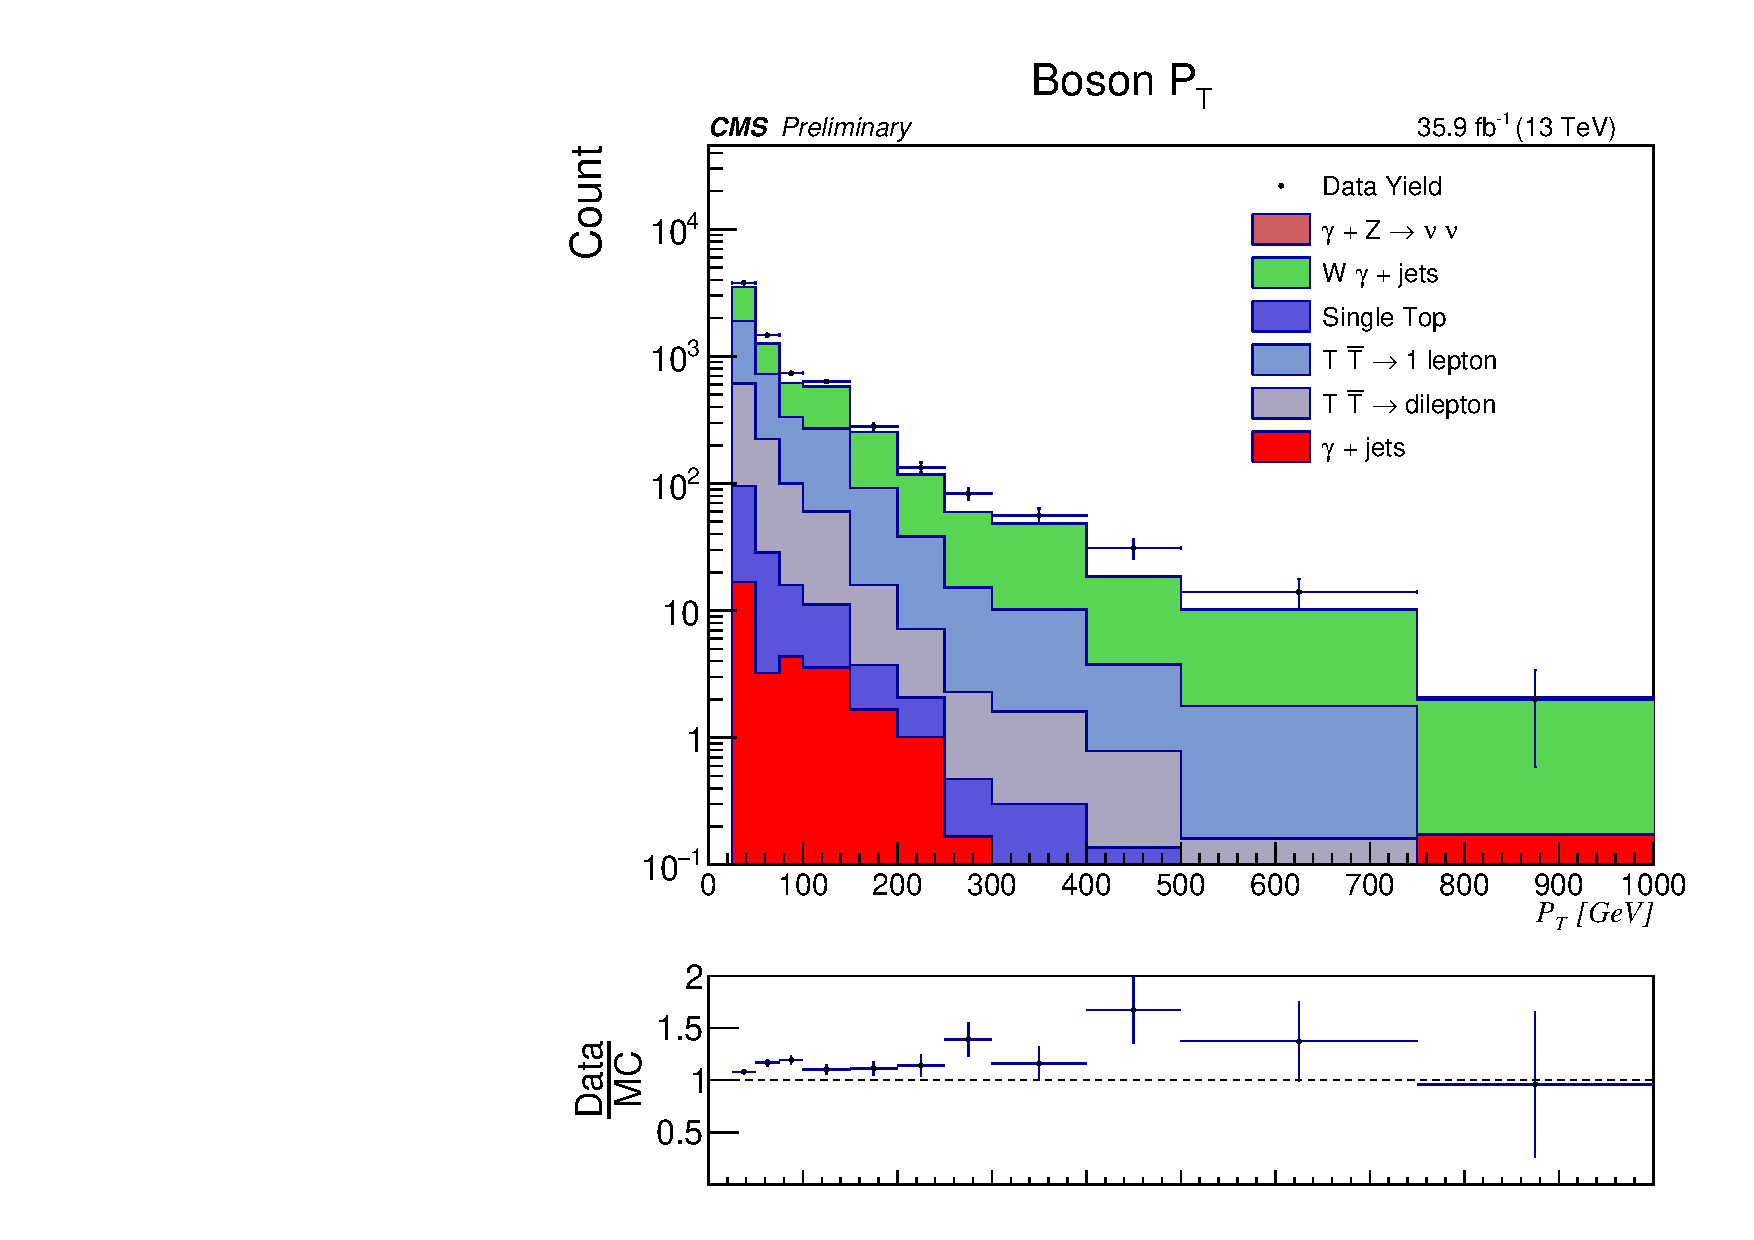
\includegraphics[width=.46\textwidth]{figures/datavsmc/mugamma/BosonPT_widebin.pdf}
        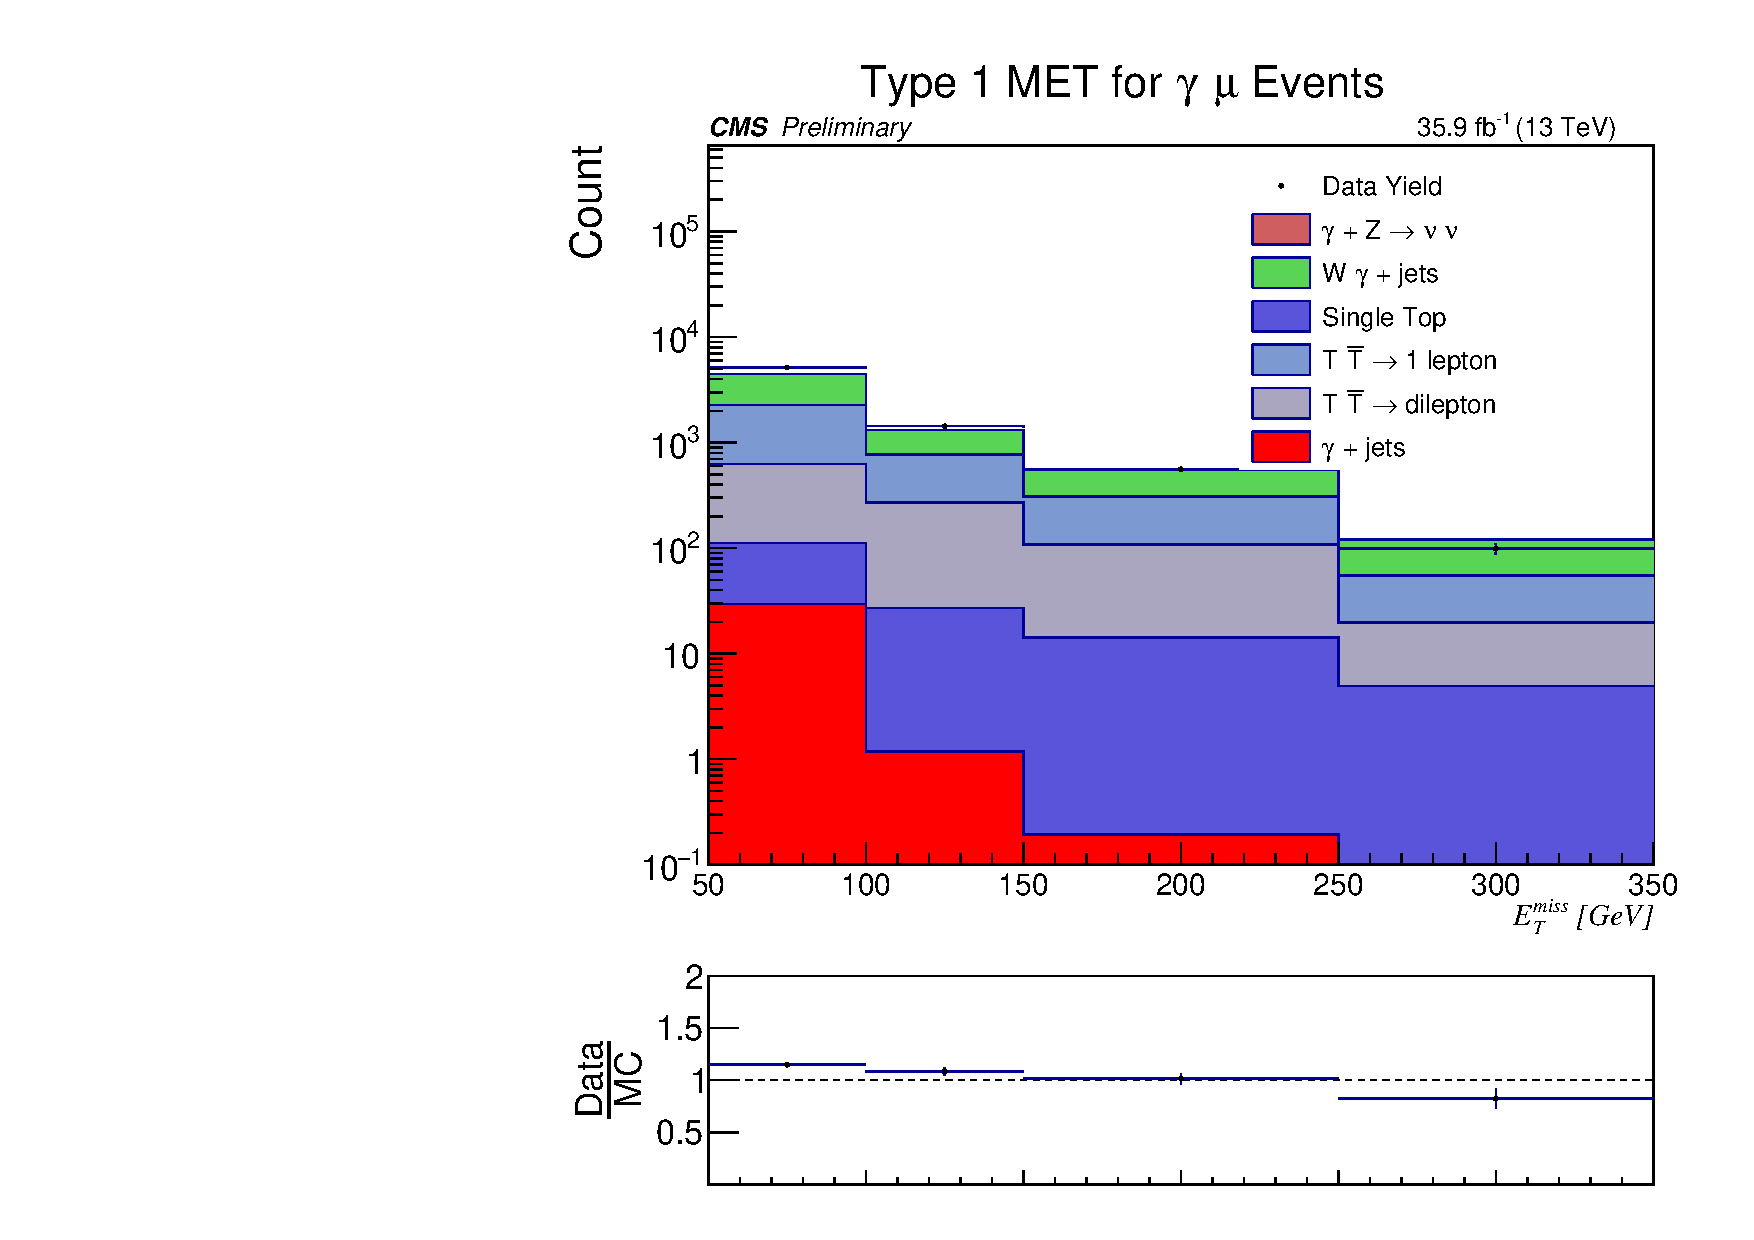
\includegraphics[width=.46\textwidth]{figures/datavsmc/mugamma/Type1MET_SRBin.pdf}
        \caption[The \pt (left) and \MET (right) profiles in simulation and data for the $\gamma \mu$ control sample, defined in sec \ref{sec:ewk_subtraction_closure_region}.]{The \pt (left) and \MET (right) profiles in simulation and data for the $\gamma \mu$ control sample, defined in sec \ref{sec:ewk_subtraction_closure_region}. The agreement between data and simulation is used to extract the expected fluctuation for the process of removing events with neutrinos from the $\gamma$+jets population. Given that the ratio is never deviates from unity by more than 30\% in the \MET profile, and mostly so in the \pt, we use 30\% as the systematic uncertainty for this process.}
        \label{fig:gamma_mu_closure}
      \end{figure}



    \subsubsection{Algorithm For The Prediction}

      Now that we have addressed the fundamental premise of this method and all the complications, we can give a full algorithm for the prediction:

      \begin{enumerate}
        \item Construct the population of single photon + jets events in the augmented search regions with dilepton quantities replaced by photon selection, full selection in sec \ref{sec:met_templates_control_region}.

        \item Simulate $\gamma+\nu$ events in MC, create a 'clean' population of only $\gamma+$jets events by subtracting the kinematic distributions of the $\gamma+\nu$ sample from any distribution of interest (in this case \pt).

        \item Take the `clean' photon sample and bin events by \pt in the intervals between (GeV): [25, 33, 40, 55, 85, 105, 135, 180, 250, $\infty$]. These are chosen to be just wide enough that there a high number of photon events in each bin, but fine enough to capture the \pt dependence of the jet configurations. 

        \item Create a `clean' Z+jets sample by taking the dilepton data that pass search region criteria, described in sec \ref{sec:search_regions}, and subtracting the other background predictions from any distribution of interest (in this case \pt). Note that the dilepton events are not binned in \MET at this point, all other cuts are applied.

        \item Normalize the area of the clean Z+jets \pt distribution and clean $\gamma+$jets to unity.

        \item Assign a weight to each photon event such that the bin has the same area as the corresponding Z+jets \pt bin.

        \item Construct the \MET profile of the cleaned $\gamma$+jets sample where each event is given the weight derived in the previous step.

        \item Find the ratio of the \MET 50-100 bin for the clean Z+jets sample vs. the clean $\gamma$+jets sample, apply this ratio across the entire cleaned $\gamma$+jets \MET profile

      \end{enumerate}

    \subsubsection{Systematics}

      The total uncertainty for this prediction is broken into 4 uncorrelated sources.

      \[
        \sigma^2_{\text{net}} = \sigma^2_{\text{Normalization}} +  \sigma^2_{\text{EWK Sub}} + \sigma^2_{\text{Statistical}} + \sigma^2_{\text{\pt Reweighting}}
      \]

      \begin{itemize}
        \bitem{Normalization} The uncertainty due to the cross section normalization of the $\gamma$+jets events to the Z+jets events in the \MET 50-100 bin. This is a percent uncertainty found on a bin-by-bin basis. The percentage is found by dividing the statistical uncertainty by the total count of events in the Z+jets \MET 50-100 bin. If the 50-100 \MET bin has a count of N events, a background prediction of $b$ in some higher \MET bin will get an uncertainty contribution of $ \sigma_{\text{Normalization}} = b \frac{\sigma(N)}{N}$ due to this source, where $\sigma(N)$ is the Poisson uncertainty for N events.

        \bitem{EWK Sub} The uncertainty due to the imperfect modeling of the $\gamma + \nu$ events when subtracting them from the $\gamma$+jets sample. A 30\% uncertainty is associated with the modeling of \pt and \MET as was shown in figure \ref{fig:gamma_mu_closure} and the section therein. This 30\% is applied to the total count of events subtracted from the \MET bin and scaled by the normalization from the \MET 50-100 bin. If $m_s$ events were subtracted from the $\gamma$+jets events in some \MET bin (after \pt reweighting), and $n$ is the normalization applied to the $\gamma$+jets sample to correct the cross section, the total uncertainty contribution to the \MET bin due to this source is $\sigma_{\text{EWK Sub}} = 0.3 \cdot n \cdot m_s$.

        \bitem{Statistical} The uncertainty due to the limited statistics of the $\gamma$+jets events. This is derived as a percent uncertainty on the \pt reweighted count of $\gamma$+jets events in a \MET bin. If a \MET bin has a background prediction of $b$ which was calculated from a $\gamma$+jets \MET bin with statistical uncertainty $\sigma_{\gamma}$, the total uncertainty contribution to the \MET bin due to this source is $\sigma_{\text{Statistical}} = \sigma_{\gamma} \cdot b$

        \bitem{\pt Reweighting} The uncertainty due to differences in the kinematics of jets in the photon and Z samples. The percent uncertainty for each \MET bin due to this source was summarized in table \ref{tab:template_systematics}. If a \MET bin has a background prediction of $b$ and the percent uncertainty due to the \pt reweighting is $p$, then the total uncertainty contribution to the \MET bin due to this source is $\sigma_{\text{\pt Reweighting}} = p \cdot b$.
      \end{itemize}

      A summary of all the Z+jets background predictions across all search bins as well as their systematics is shown below in table \ref{tab:template_systematics_summary}.

      \begin{table}[!h]
        \scriptsize
        \centering
        \caption{\label{tab:template_systematics_summary} A summary of all prediction counts and uncertainties for the Z+jets predictions. The number ``ratio" is the particular uncertainty associated for the process divided by the total uncertainty for the prediction in the \MET bin.
          }
        \begin{center}
          \begin{tabular} {l |l | l | l | l | l | l}
            SR & MET Bin & Prediction & Closure (ratio) & Normalization (ratio) & Statistical (ratio) & EWK Sub (ratio) \\ \hline
            SRA & 100-150 & 13.61 $\pm$ 3.14 & 2.72 (0.87) & 1.00 (0.32) & 1.14 (0.36) & 0.34 (0.11) \\
            & 150-250 & 2.45 $\pm$ 0.87 & 0.64 (0.74) & 0.18 (0.21) & 0.36 (0.42) & 0.42 (0.49) \\
            & 250+ & 3.26 $\pm$ 2.36 & 0.85 (0.36) & 0.24 (0.10) & 2.16 (0.91) & 0.39 (0.16) \\ \hline


            SRAb & 100-150 & 8.21 $\pm$ 2.10 & 1.64 (0.78) & 0.89 (0.42) & 0.92 (0.44) & 0.27 (0.13) \\
            & 150-250 & 1.19 $\pm$ 0.54 & 0.31 (0.57) & 0.13 (0.24) & 0.24 (0.45) & 0.35 (0.65) \\
            & 250+ & 0.51 $\pm$ 0.27 & 0.13 (0.48) & 0.05 (0.20) & 0.15 (0.56) & 0.18 (0.64) \\ \hline


            SRB & 100-150 & 12.81 $\pm$ 2.35 & 1.54 (0.65) & 1.19 (0.51) & 1.30 (0.56) & 0.16 (0.07) \\
            & 150-250 & 0.89 $\pm$ 0.34 & 0.13 (0.39) & 0.08 (0.24) & 0.22 (0.66) & 0.20 (0.59) \\
            & 250+ & 0.38 $\pm$ 0.20 & 0.06 (0.29) & 0.04 (0.18) & 0.12 (0.63) & 0.14 (0.69) \\ \hline


            SRBb & 100-150 & 7.74 $\pm$ 3.11 & 0.93 (0.30) & 1.32 (0.42) & 2.65 (0.85) & 0.23 (0.07) \\
            & 150-250 & 4.04 $\pm$ 3.33 & 0.73 (0.22) & 0.69 (0.21) & 3.16 (0.95) & 0.25 (0.07) \\
            & 250+ & 0.10 $\pm$ 0.14 & 0.02 (0.13) & 0.02 (0.12) & 0.04 (0.28) & 0.14 (0.94) \\ \hline


            SRC & 100-150 & 1.24 $\pm$ 0.43 & 0.19 (0.43) & 0.27 (0.64) & 0.27 (0.63) & 0.04 (0.09) \\
            & 150+ & 0.13 $\pm$ 0.11 & 0.04 (0.36) & 0.03 (0.27) & 0.05 (0.51) & 0.08 (0.74) \\ \hline


            SRCb & 100-150 & 0.14 $\pm$ 0.47 & 0.03 (0.06) & 0.05 (0.10) & 0.04 (0.08) & 0.47 (0.99) \\
            & 150+ & 0.00 $\pm$ 0.33 & 0.00 (0.00) & 0.00 (0.00) & 0.00 (0.00) & 0.33 (1.00) \\ \hline


            VZ & 100-150 & 29.27 $\pm$ 4.42 & 3.22 (0.73) & 1.13 (0.26) & 2.15 (0.49) & 1.81 (0.41) \\
            & 150-250 & 2.87 $\pm$ 2.09 & 0.69 (0.33) & 0.11 (0.05) & 0.40 (0.19) & 1.93 (0.92) \\
            & 250-350 & 1.00 $\pm$ 0.73 & 0.24 (0.33) & 0.04 (0.05) & 0.24 (0.33) & 0.64 (0.88) \\
            & 350+ & 0.29 $\pm$ 0.30 & 0.07 (0.23) & 0.01 (0.04) & 0.08 (0.26) & 0.28 (0.94) \\ \hline


            HZ & 100-150 & 2.90 $\pm$ 2.39 & 2.32 (0.97) & 0.34 (0.14) & 0.41 (0.17) & 0.24 (0.10) \\
            & 150-250 & 0.26 $\pm$ 0.19 & 0.09 (0.47) & 0.03 (0.16) & 0.08 (0.44) & 0.14 (0.75) \\
            & 250+ & 0.09 $\pm$ 0.07 & 0.03 (0.45) & 0.01 (0.16) & 0.05 (0.77) & 0.03 (0.42) \\ \hline

          \end{tabular}
        \end{center}
      \end{table}

  \clearpage

  \subsection{Flavor Symmetric Background} \label{sec:flavor_symmetric_background}
    
    The flavor symmetric background accounts for all cases where even a single lepton in the final dilepton pair was produced through the decay of a W boson. The basic idea is that the W has almost exactly the same decay rate to electrons and muons, therefore any event where a lepton was produced in a W decay should be mirrored by another event where the lepton was produced with the other flavor. In other words, if a physics process where a dilepton pair is produced and \emph{at least} one lepton came from a W boson occurs at some frequency $f$, a process where the dilepton pair has different flavor should occur with the same rate, $f$. The same argument holds for any flavor-symmetric process. For instance, ZZ production with two lost leptons, one from each Z, is also a flavor symmetric background because the chance to lose a muon is no different from the chance to lose an electron.\footnote{This is a rare process and those lost-lepton probabilities are not precisely identical, but the reader should understand that the existence of a W boson is not necessary to make a background process flavor symmetric. It is simply the most likely scenario as $t\bar{t}$ production is the only large cross section flavor-symmetric process in our search space.}

    Furthermore, given that the mass of the electron and the mass of the muon are many orders of magnitude less than the dilepton mass requirement of roughly 90 GeV, the typical energy scales and orientation of light leptons in flavor symmetric processes should be the same regardless of whether the leptons are paired with a same flavor or different flavor partner. This means that we can use the kinematical distributions in events with different flavor lepton pairs to predict the kinematical distributions for events with a same flavor lepton pair.

    In a totally idealized scenario, the flavor symmetric background prediction would be extremely simple. First, we would invert the selection for same flavor lepton pairs to require different flavor pairs in each \MET bin of our search regions. Then the count in each \MET for the different flavor pairs could be taken as the expected count for the search bin. However, as with any background prediction method, there are complications to our idealized scenario. 

    The first is that the \emph{reconstruction efficiency} for electrons and muons is not identical, meaning that there is a slight asymmetry between how likely the CMS detector and software suite are to find a muon vs. how likely they are to find an electron at some particular energy. This effect is caused by different detection methods used for electrons and muons. It manifests as different trigger efficiencies for electrons and muons at the same \pt, as briefly explained in sec \ref{sec:trigger_efficiencies}, as well the differences in the electron and muon ID requirements outlined in sections \ref{sec:electron_id_and_isolation} and \ref{sec:muon_id_and_isolation}. We correct for this effect with a factor called \rsfof, which is the subject of the next section.

    The second is that with few enough events, the symmetry between same-flavor and different-flavor pairs can be thrown off by statistical fluctuations.\footnote{Tossing a coin should yield as many heads as tails, however it is just as likely to get HH \emph{or} TT in tossing a coin twice as it is to get one of each. To chance to get an uneven percentage of heads or tails in a series of throws decreases with number of throws. The symmetry has more power with more statistics.} For this analysis, the expected number of flavor symmetric events in most search bins is less than 2. In order to ensure we have enough statistics for each prediction, the mass window for the acceptance of different flavor events is enlarged.

    With all corrections applied, the final number of events predicted in a \MET bin is 

    \begin{equation}
      N_{\text{SF}} = \kappa \cdot \rsfof \cdot N_{\text{DF}}, \label{eq:n_sf}
    \end{equation}

    where $\kappa$ is a corrective factor associated with the extrapolation from the enlarged mass window into the Z mass window, and \rsfof is a corrective factor associated with the asymmetry in electron and muon efficiencies.

    \subsubsection{The \rsfof Factor} \label{sec:rsfof}

      The factor \rsfof in eq. \ref{eq:n_sf} is a transfer factor which is meant to scale the number of different-flavor events in the flavor symmetric control regions, essentially the search regions with their same flavor requirement inverted, to the number of same-flavor events in associated search bin. This factor is derived through a direct measurement in the \rsfof control region, defined in sec. \ref{sec:rsfof_measurement_region} as $\MET \in [100,150]$, $\njets = 2$, and $\mll \notin [70,110]$. 

      The measurement of this factor is done in both data and $t\bar{t}$ MC, but the value MC is used only as a sanity check on the method. In order to set an uncertainty associated with this method, the \rsfof control region is binned further by various parameters that are used to construct the search regions. The variation in the measured value across these bins is used as the expected fluctuation of the method. These checks are shown in figure \ref{fig:rsfof_unc}.

      \begin{figure}[h!]
        \centering
        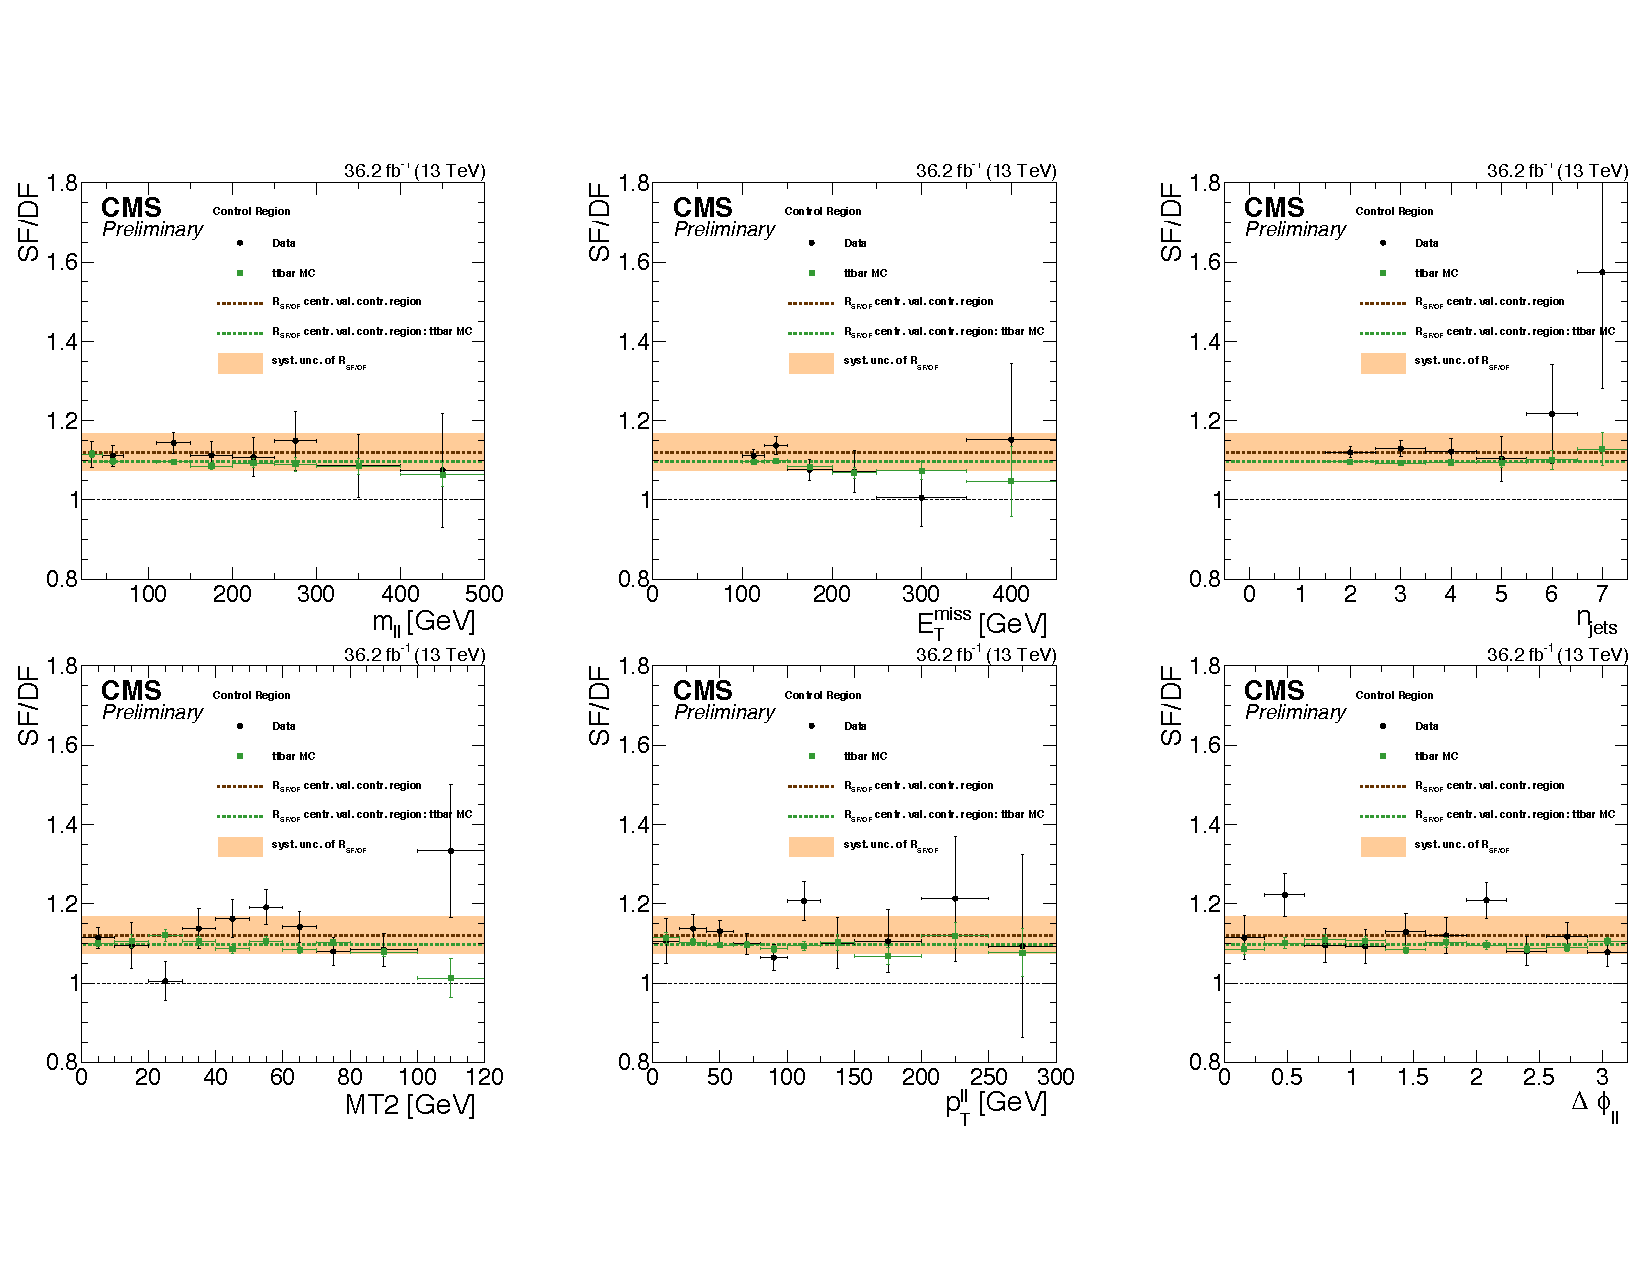
\includegraphics[width=\textwidth]{figures/RSFOF_Uncertainty.pdf}
        \caption[The measurement of \rsfof and its uncertainty.]{The measurement of \rsfof and its uncertainty. The \rsfof control region is further binned along the variables shown, and \rsfof is measured as they vary. The orange band shows the one-$\sigma$ expected fluctuation set by this method. As can be seen, the majority of data points fall within this orange band. \rsfof is relatively well behaved as a function of these kinematic and event-level variables.}
        \label{fig:rsfof_unc}
      \end{figure}

      The final value of \rsfof measured in data is $1.107 \pm 0.046$ (which is the value used in the final prediction), and the cross check in MC gives $1.090 \pm 0.005$.


    \subsubsection{Enlarging The Mass Window} \label{sec:kappa}

      In order to keep the statistical uncertainty reasonable, we enlarge the flavor symmetric control region's \mll window from $\pm 5$ GeV about the Z mass to $> 20$ GeV. Then we must apply a transfer factor, denoted by $\kappa$, which gives the ratio of number of events expected in this enlarged window, to the number of events expected in the Z mass window. 

      \[
        \kappa = \frac{\text{Num Different Flavor Events in Z Mass Window}}{\text{Num Different Flavor Events with \mll } > 20 \text{ GeV}}
      \]

      Furthermore, although \mll was chosen precisely because it is a relatively flat variable for $t\bar{t}$ events near the search regions, there are going to be some kinematic differences introduced by this asymmetry. In order to set an uncertainty associated with this method, we measure $\kappa$ in several control, search, and amalgamated search regions, defined in sec. \ref{sec:kappa_measurement_regions}. Simulated $t\bar{t}$ events are also used to measure $\kappa$ in these regions as a sanity check on the method to ensure there is little to no background contamination in the flavor symmetric control region. 

      The measured value of $\kappa$ is $0.065 \pm 0.02$ The $\kappa$ central value is then chosen to fit the various measured values. The one-$\sigma$ expected fluctuation is chosen such most values measured in data and all values measured in MC are within the band. Figure \ref{fig:kappa} summarized the measurements of $\kappa$ across all search and control regions in both data and MC. 

      \begin{figure}[h!]
        \centering
        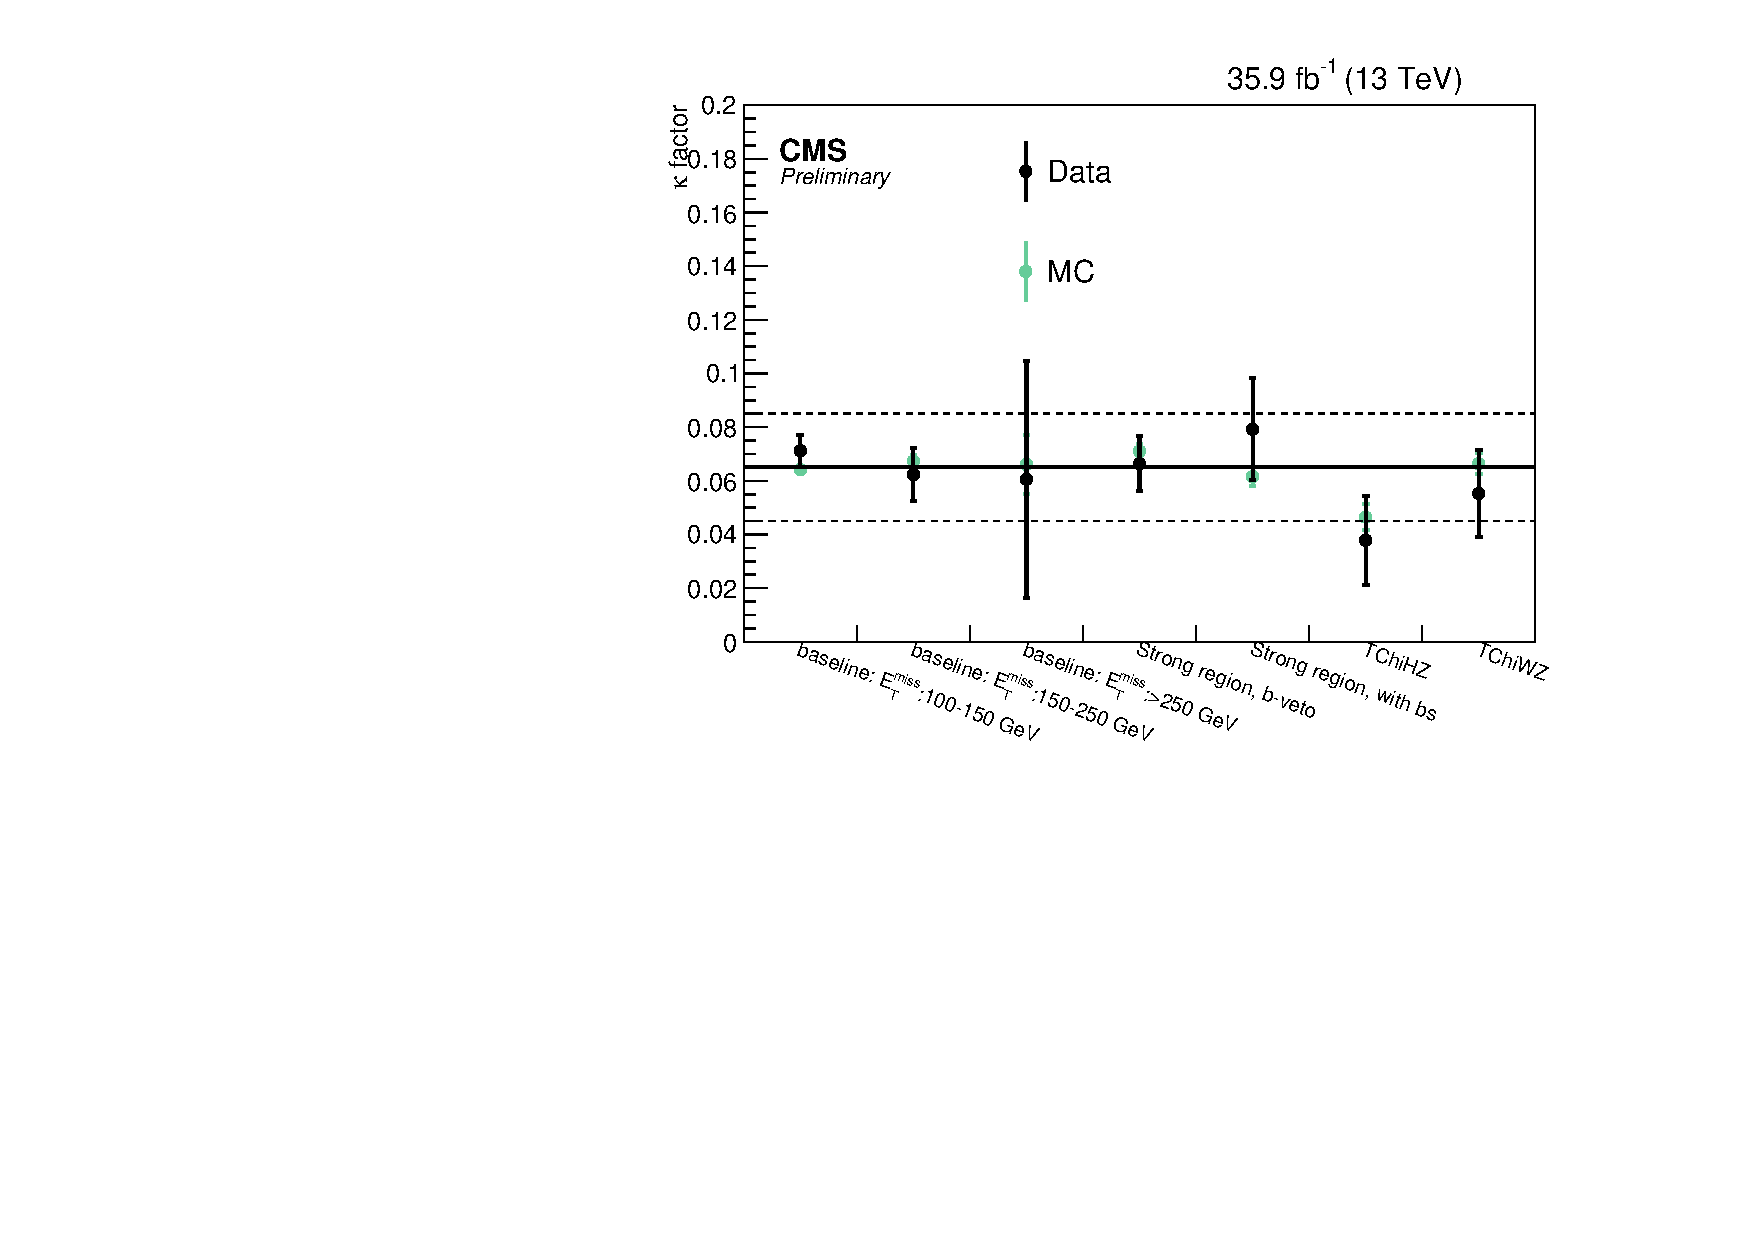
\includegraphics[width=\textwidth]{figures/datavsmc/data_summary_kfactors.pdf}
        \caption{The measurement of $\kappa$ across various search and control regions. The value measured in data and MC agree within uncertainty for all regions. The solid line is the central value chosen for $\kappa$ and the dashed lines represent the one-$\sigma$ expected fluctuations.}
        \label{fig:kappa}
      \end{figure}

      \clearpage

    \subsubsection{Systematics}

      The total uncertainty for this prediction is broken into 3 uncorrelated sources.

      \[
        \sigma^2_{\text{net}} = \sigma^2_{\text{\rsfof}} +  \sigma^2_{\kappa} + \sigma^2_{\text{Statistical}}
      \]

      The quantities $\sigma_{\text{\rsfof}}$ and $\sigma_{\kappa}$ are derived by taking the difference in the prediction when varying \rsfof and $\kappa$ between the two ends of their measured windows reported above. $\sigma_{\text{Statistical}}$ is the Poisson uncertainty on the number of events in the flavor symmetric control region associated the search bin scaled by the product of \rsfof and $\kappa$.

  \subsection{Z + $\nu$} \label{sec:z_+_neutrino}

    Table \ref{tab:znu_processes} summarizes the non-negligible background processes considered that can produce the Z+$\nu$ signature. The simulated events are only accepted when the dilepton pair can be matched back to a pair that came from a Z boson and there is a neutrino in the final state. This selection ensures there is no double counting background events that should be predicted by the flavor symmetric or Z+hadronic predictions.


    \begin{table}[!h]
      \centering
      \caption{\label{tab:znu_processes}
      A summary of the Z+$\nu$ background sources. These processes are simulated as described in sec \ref{sec:monte_carlo}. Only events which have a prompt neutrino and where the pair of selected leptons can be matched to a Z boson are considered to ensure orthogonality with the Z+jets and flavor symmetric background predictions.
      }
      \begin{center}
        \begin{tabular} {l | l}
        \hline
        \hline
        Category & Processes \\
        \hline
        WZ     & WZ$\to 3\ell + \nu$           \\
        ZZ     & 2$\ell + 2\nu$                \\
        TTZ    & Z$\to 2\ell$ and Z$\to 2\nu$  \\
        VVV    & ZZZ (inclusive decays)        \\
               & WZZ (inclusive decays)        \\
               & WWZ (inclusive decays)        \\
        \hline
        \hline
        \end{tabular}
      \end{center}
    \end{table}


    \subsubsection{Normalization Factors}
      Monte Carlo cross section are notoriously unreliable for low cross-section physics, especially in extreme regions of phase space used for new physics searches. In order to check the cross sections in the simulated events, the ZZ, WZ, and TTZ simulation are compared against data in specific control regions constructed to be sensitive to these processes. The full definitions of these control regions are given in sec \ref{sec:znu_control_regions}. Figure \ref{fig:rare_xsec_check} summarizes the results of these comparisons. 

      \begin{figure}[!h]
        \begin{center}
          \begin{tabular}{ccc}
            \begin{overpic}[width=0.3\textwidth]{figures/datavsmc/rare_xsec/WZ.pdf}    \put(30,68){\parbox{.5in}{\color{black} \small WZ Control Region}}     \end{overpic} &
            \begin{overpic}[width=0.3\textwidth]{figures/datavsmc/rare_xsec/ZZ.pdf}   \put(18,68){\parbox{.5in}{\color{black} \small ZZ \\ Control Region}}    \end{overpic} &
            \begin{overpic}[width=0.3\textwidth]{figures/datavsmc/rare_xsec/TTZ.pdf}    \put(18,68){\parbox{.5in}{\color{black} \small TTZ Control Region}}     \end{overpic} \\
          \end{tabular}
          \caption[Data and MC are compared in WZ, ZZ, and TTZ control regions in order to check whether the cross section in MC is compatible with what we see in data.]{ \normalsize Data and MC are compared in WZ, ZZ, and TTZ control regions in order to check whether the cross section in MC is compatible with what we see in data. A normalized is derived from simulation such that the number of events in the control region in data and MC agree. The ratio is extracted in the $86 ~\text{GeV} > \text{m}_{ll} > 96 ~\text{GeV}$ in the ZZ and TTZ regions, and in $60 ~\text{GeV} > \MET > 200 ~\text{GeV}$ in the WZ region. \label{fig:rare_xsec_check}
          }
        \end{center}
      \end{figure}

      Due to the low cross section, difficulty of isolation, and low impact on the results, a rigorous analysis on the performance of simulation for these processes is not undertaken. Rather, a large conservative uncertainty is chosen based on the historical performance of simulating these models. A summary of derived normalization factors and the associated uncertainty in MC modeling is given in table \ref{tab:znu_norm_factors}.

      \begin{table}[!h]
      \centering
      \caption[A summary of the Z+$\nu$ background sources' normalization factors and uncertainties.]{\label{tab:znu_norm_factors}
      A summary of the Z+$\nu$ background sources' normalization factors and uncertainties. For the WZ, ZZ, and TTZ processes, normalization factors were found to correct the MC cross section, the VVV processes have low enough cross section that this is neglected. Due to the difficulty of isolating these processes and their low impact on search results, flat uncertainties are taken based on our level of confidence in MC performance.
      }
      \begin{center}
        \begin{tabular} {l | l | l}
        \hline
        \hline
        Sample & Normalization Factor & Percent Uncertainty \\
        \hline
        WZ     & 1.06                 & 30\%                \\
        ZZ     & 1.71                 & 50\%                \\
        TTZ    & 1.36                 & 30\%                \\
        VVV    & 1                    & 50\%                \\
        \hline
        \hline
        \end{tabular}
      \end{center}
    \end{table}

  \subsubsection{Systematics}

      The total uncertainty for this prediction is broken into 2 uncorrelated sources.

      \[
        \sigma^2_{\text{net}} = \sigma^2_{\text{MC Performance}} + \sigma^2_{\text{Statistical}}
      \]

      The statistical uncertainty is taken from the MC, the ``MC Performance" uncertainty is given in table \ref{tab:znu_norm_factors} above.

\section{Results} \label{sec:results}
  \subsection{Strong Search Regions} \label{sec:strong_search_regions}
    In this section, we show the search results for the strong signal regions. Figure \ref{fig:results_SR_str} shows the results visually, each search region is shown binned in \MET, the background predictions are broken down as described in \ref{sec:background_estimation_methods} and uncertainty bands are shown as a hashing that captures all sources described above. The number of events in data seen are shown as black dots in the figures. The same data is shown numerically in table \ref{tab:results_SR_str}.

    \begin{table}[!h]
      \centering
      \caption[Numerical results for the strong search regions.]{\label{tab:results_SR_str}
      Numerical results for the strong search regions are shown. The precise definitions of these regions are shown in table \ref{tab:selections_sr}. See figure~\ref{fig:results_SR_str}~for the corresponding plots. The agreement in the MET 50-100 bin is by construction as that bin is used to normalize the Z+Hadronic prediction. No statistically significant deviation from the standard model prediction is found.
      }
      \begin{center}
        \begin{tabular} {l | l | l | l | l | l }
          SRA & \MET [GeV]  & 50-100 & 100-150 & 150-250 & 250+ \\ \hline 
          & Z+Hadronic  & 208.5$\pm$16.1 & 13.6$\pm$3.1 & 2.5$\pm$0.9 & 3.3$\pm$2.4 \\
          & FS  & $0.4^{+0.3}_{-0.2}$  & $0.4^{+0.3}_{-0.2}$  & $0.2^{+0.2}_{-0.1}$  & $0.2^{+0.2}_{-0.1}$  \\
          & Z+$\nu$  & 1.1$\pm$0.4 & 0.8$\pm$0.3 & 1.4$\pm$0.4 & 2.4$\pm$0.8 \\ 
          & Sum  & $210.0^{+16.1}_{-16.1}$  & $14.8^{+3.2}_{-3.2}$  & $4.0^{+1.0}_{-1.0}$  & $5.9^{+2.5}_{-2.5}$ \\ 
          & Data  & 210 & 23 & 5 & 4 \\ \hline 


          SRAb & \MET [GeV]  & 50-100 & 100-150 & 150-250 & 250+ \\ \hline 
          & Z+Hadronic  & 92.2$\pm$10.4 & 8.2$\pm$2.1 & 1.2$\pm$0.5 & 0.5$\pm$0.3 \\
          & FS  & $1.9^{+0.7}_{-0.7}$  & $2.3^{+0.8}_{-0.8}$  & $1.7^{+0.7}_{-0.6}$  & $0.1^{+0.2}_{-0.1}$  \\
          & Z+$\nu$  & 1.9$\pm$0.4 & 1.9$\pm$0.4 & 2.0$\pm$0.5 & 1.8$\pm$0.6 \\ 
          & Sum  & $96.0^{+10.4}_{-10.4}$  & $12.4^{+2.3}_{-2.3}$  & $4.9^{+1.0}_{-1.0}$  & $2.5^{+0.7}_{-0.7}$ \\ 
          & Data  & 96 & 14 & 7 & 1 \\ \hline 


          SRB & \MET [GeV]  & 50-100 & 100-150 & 150-250 & 250+ \\ \hline 
          & Z+Hadronic  & 130.1$\pm$12.8 & 12.8$\pm$2.3 & 0.9$\pm$0.3 & 0.4$\pm$0.2 \\
          & FS  & $0.3^{+0.2}_{-0.2}$  & $0.4^{+0.3}_{-0.2}$  & $0.4^{+0.3}_{-0.2}$  & $0.1^{+0.2}_{-0.1}$  \\
          & Z+$\nu$  & 0.6$\pm$0.2 & 0.3$\pm$0.1 & 0.7$\pm$0.2 & 1.2$\pm$0.4 \\ 
          & Sum  & $131.0^{+12.8}_{-12.8}$  & $13.6^{+2.4}_{-2.4}$  & $2.0^{+0.5}_{-0.5}$  & $1.6^{+0.5}_{-0.4}$ \\ 
          & Data  & 131 & 10 & 4 & 0 \\ \hline 


          SRBb & \MET [GeV]  & 50-100 & 100-150 & 150-250 & 250+ \\ \hline 
          & Z+Hadronic  & 37.9$\pm$6.7 & 7.7$\pm$3.1 & 4.0$\pm$3.3 & 0.1$\pm$0.1 \\
          & FS  & $0.7^{+0.4}_{-0.3}$  & $1.4^{+0.6}_{-0.5}$  & $1.1^{+0.5}_{-0.4}$  & $0.2^{+0.2}_{-0.1}$  \\
          & Z+$\nu$  & 1.3$\pm$0.4 & 2.0$\pm$0.5 & 2.3$\pm$0.6 & 1.0$\pm$0.3 \\ 
          & Sum  & $40.0^{+6.8}_{-6.8}$  & $11.1^{+3.2}_{-3.2}$  & $7.4^{+3.4}_{-3.4}$  & $1.3^{+0.4}_{-0.3}$ \\ 
          & Data  & 40 & 10 & 5 & 0 \\ \hline 


          SRC & \MET [GeV]  &  50-100 &  100-150 & \multicolumn{2}{l}{ 150+ } \\ \hline 
          & Z+Hadronic  &  23.8$\pm$5.5 &  1.2$\pm$0.4 & \multicolumn{2}{l}{ 0.1$\pm$0.1 } \\ 
          & FS  &  $0.1^{+0.2}_{-0.1}$  &  $0.4^{+0.3}_{-0.2}$  & \multicolumn{2}{l}{ $0.1^{+0.2}_{-0.1}$  } \\ 
          & Z+$\nu$  &  0.2$\pm$0.1 &  0.1$\pm$0.1 & \multicolumn{2}{l}{ 0.5$\pm$0.2 } \\ 
          & Sum  &  $24.0^{+5.5}_{-5.5}$  &  $1.7^{+0.5}_{-0.5}$  & \multicolumn{2}{l}{ $0.7^{+0.3}_{-0.2}$ } \\ 
          & Data  &  24 &  4 & \multicolumn{2}{l}{ 0 } \\ \hline 


          SRCb & \MET [GeV]  &  50-100 &  100-150 & \multicolumn{2}{l}{ 150+ } \\ \hline 
          & Z+Hadronic  &  9.9$\pm$3.7 &  0.1$\pm$0.5 & \multicolumn{2}{l}{ 0.0$\pm$0.3 } \\ 
          & FS  &  $0.1^{+0.2}_{-0.1}$  &  $0.0^{+0.1}_{-0.0}$  & \multicolumn{2}{l}{ $0.3^{+0.2}_{-0.2}$  } \\ 
          & Z+$\nu$  &  0.0$\pm$0.1 &  0.6$\pm$0.2 & \multicolumn{2}{l}{ 0.6$\pm$0.2 } \\ 
          & Sum  &  $10.0^{+3.7}_{-3.7}$  &  $0.8^{+0.5}_{-0.5}$  & \multicolumn{2}{l}{ $0.9^{+0.5}_{-0.4}$ } \\ 
          & Data  &  10 &  2 & \multicolumn{2}{l}{ 2 } \\ \hline 

        \end{tabular}
      \end{center}
    \end{table}

    \begin{figure}[!htb]
      \centering
      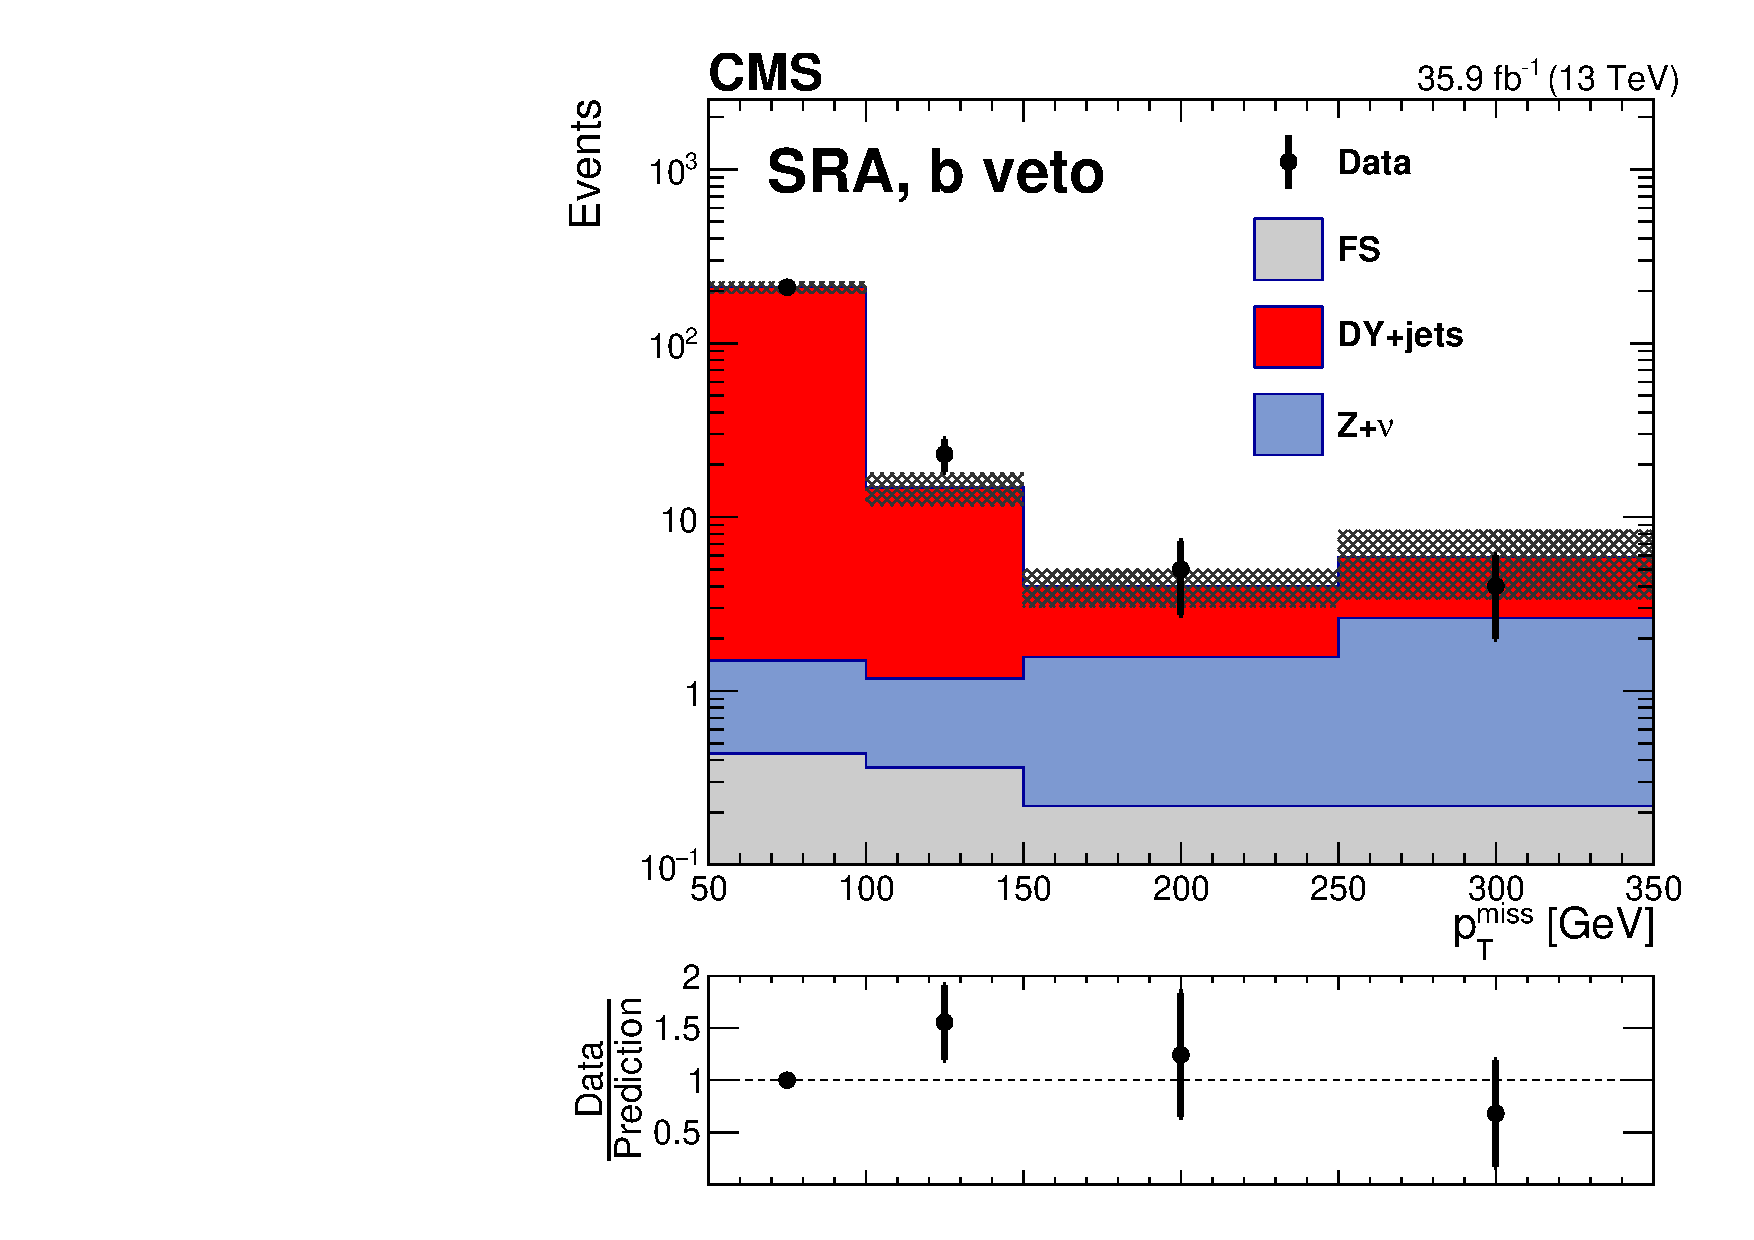
\includegraphics[width=0.35\linewidth]{figures/results/h_met_SR_2jbv.pdf}%
      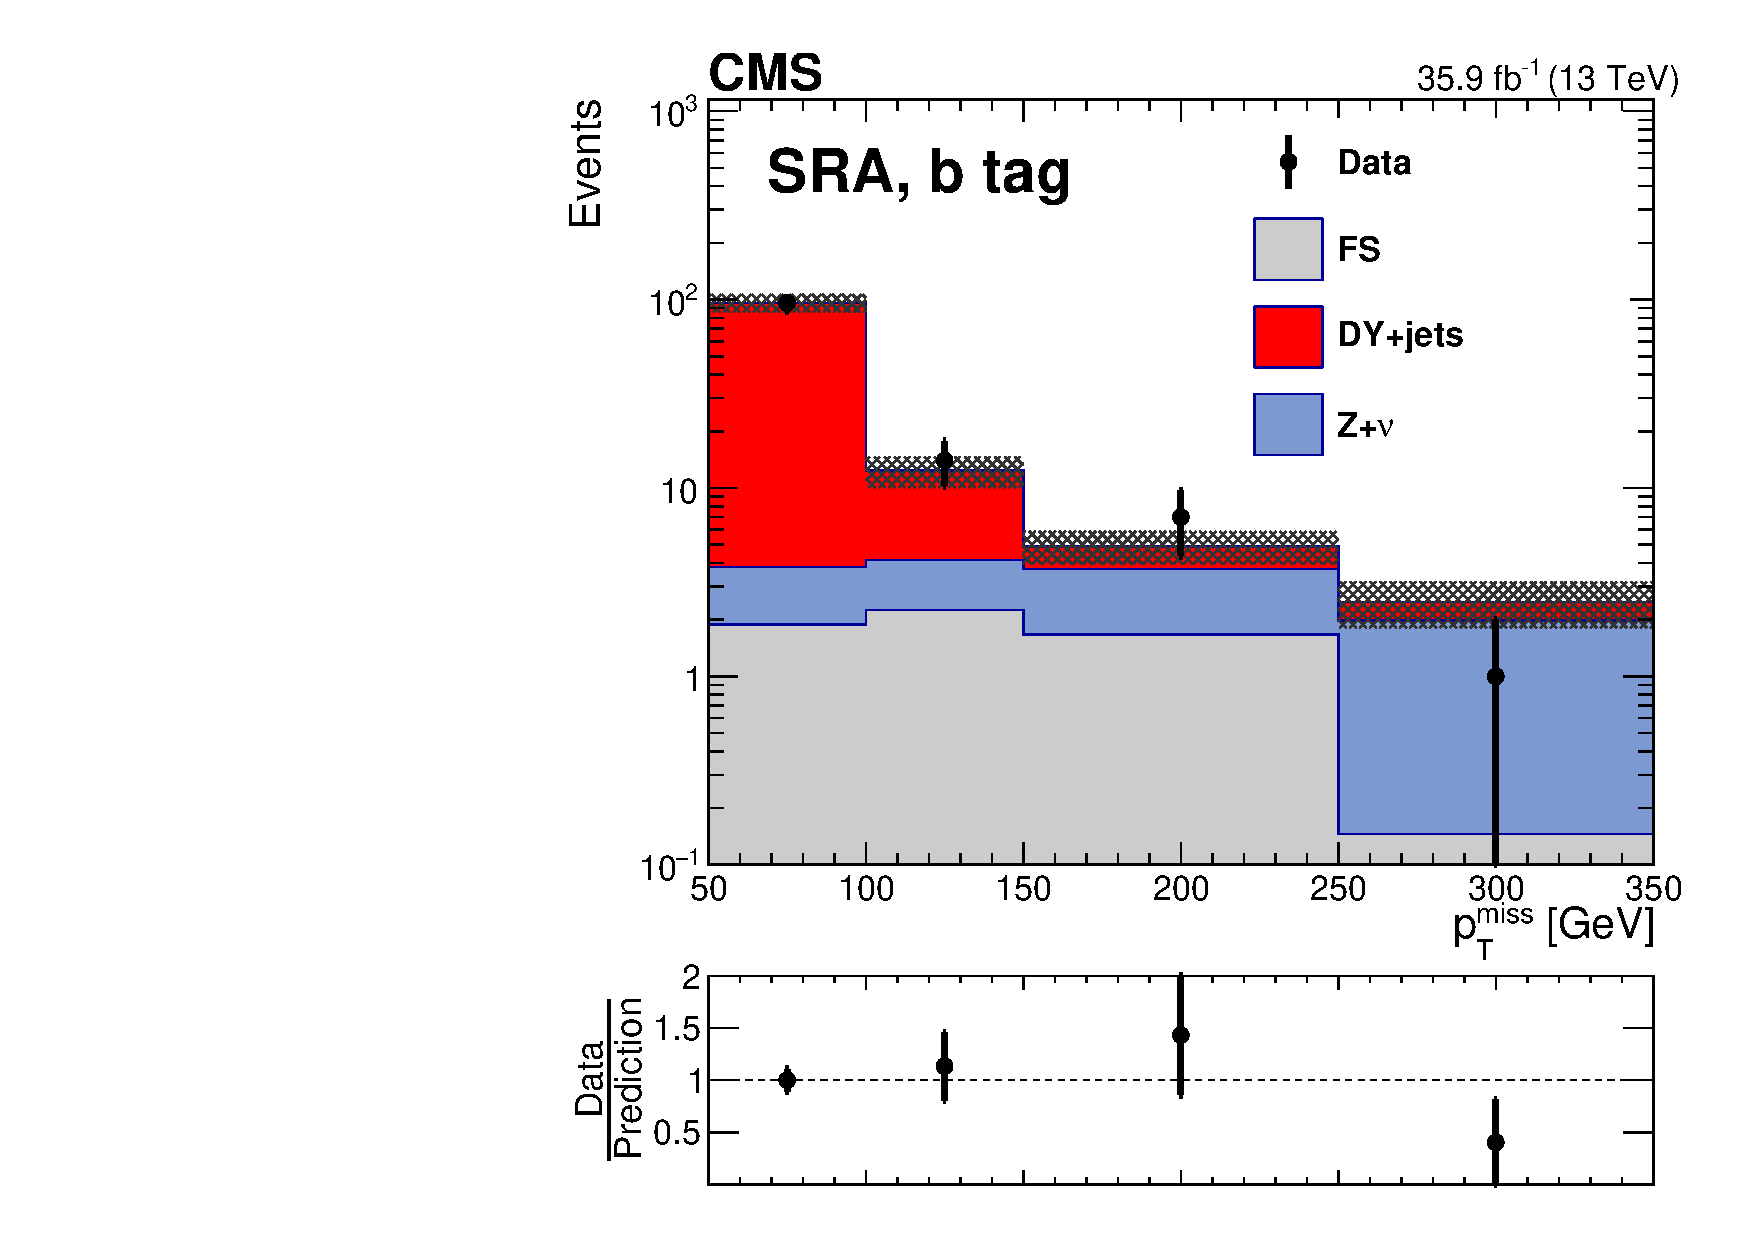
\includegraphics[width=0.35\linewidth]{figures/results/h_met_SR_2jbt.pdf}
      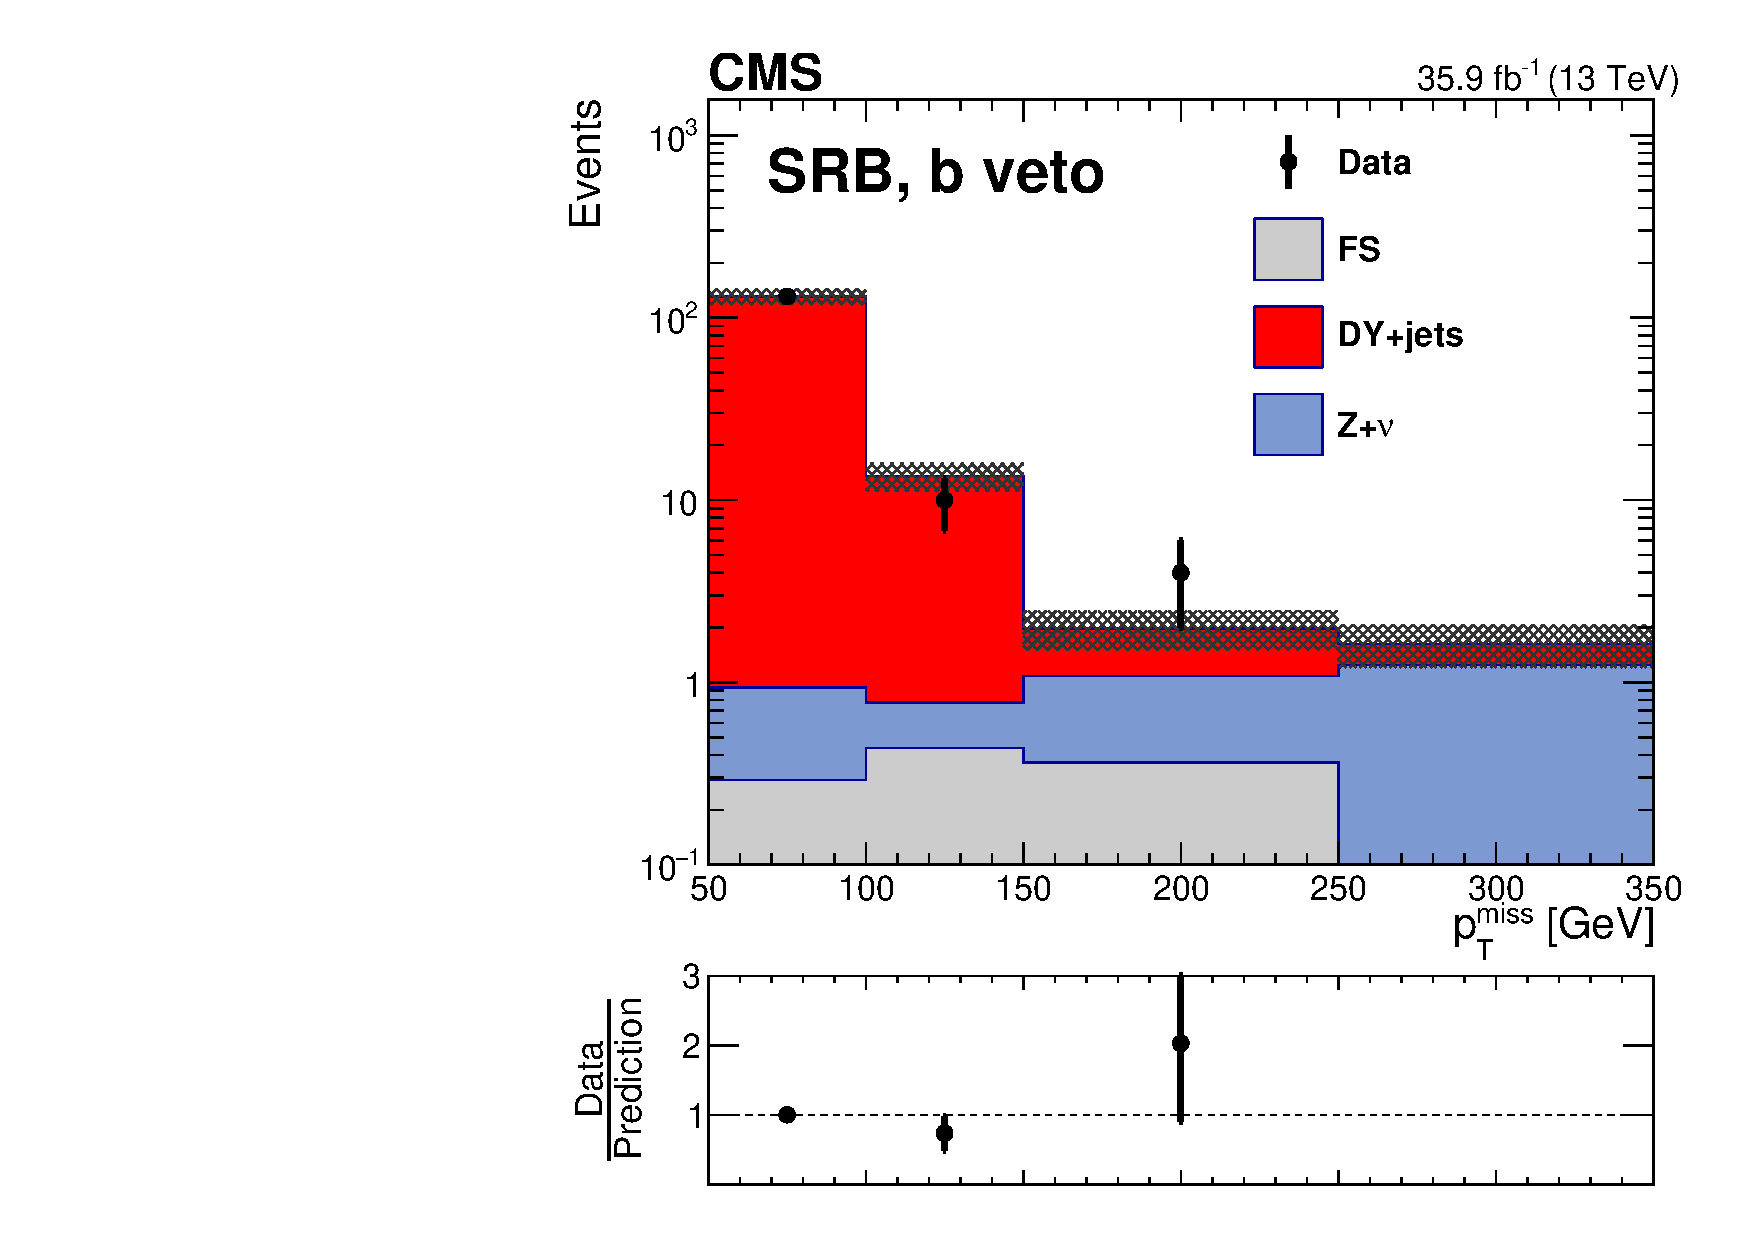
\includegraphics[width=0.35\linewidth]{figures/results/h_met_SR_4jbv.pdf}%
      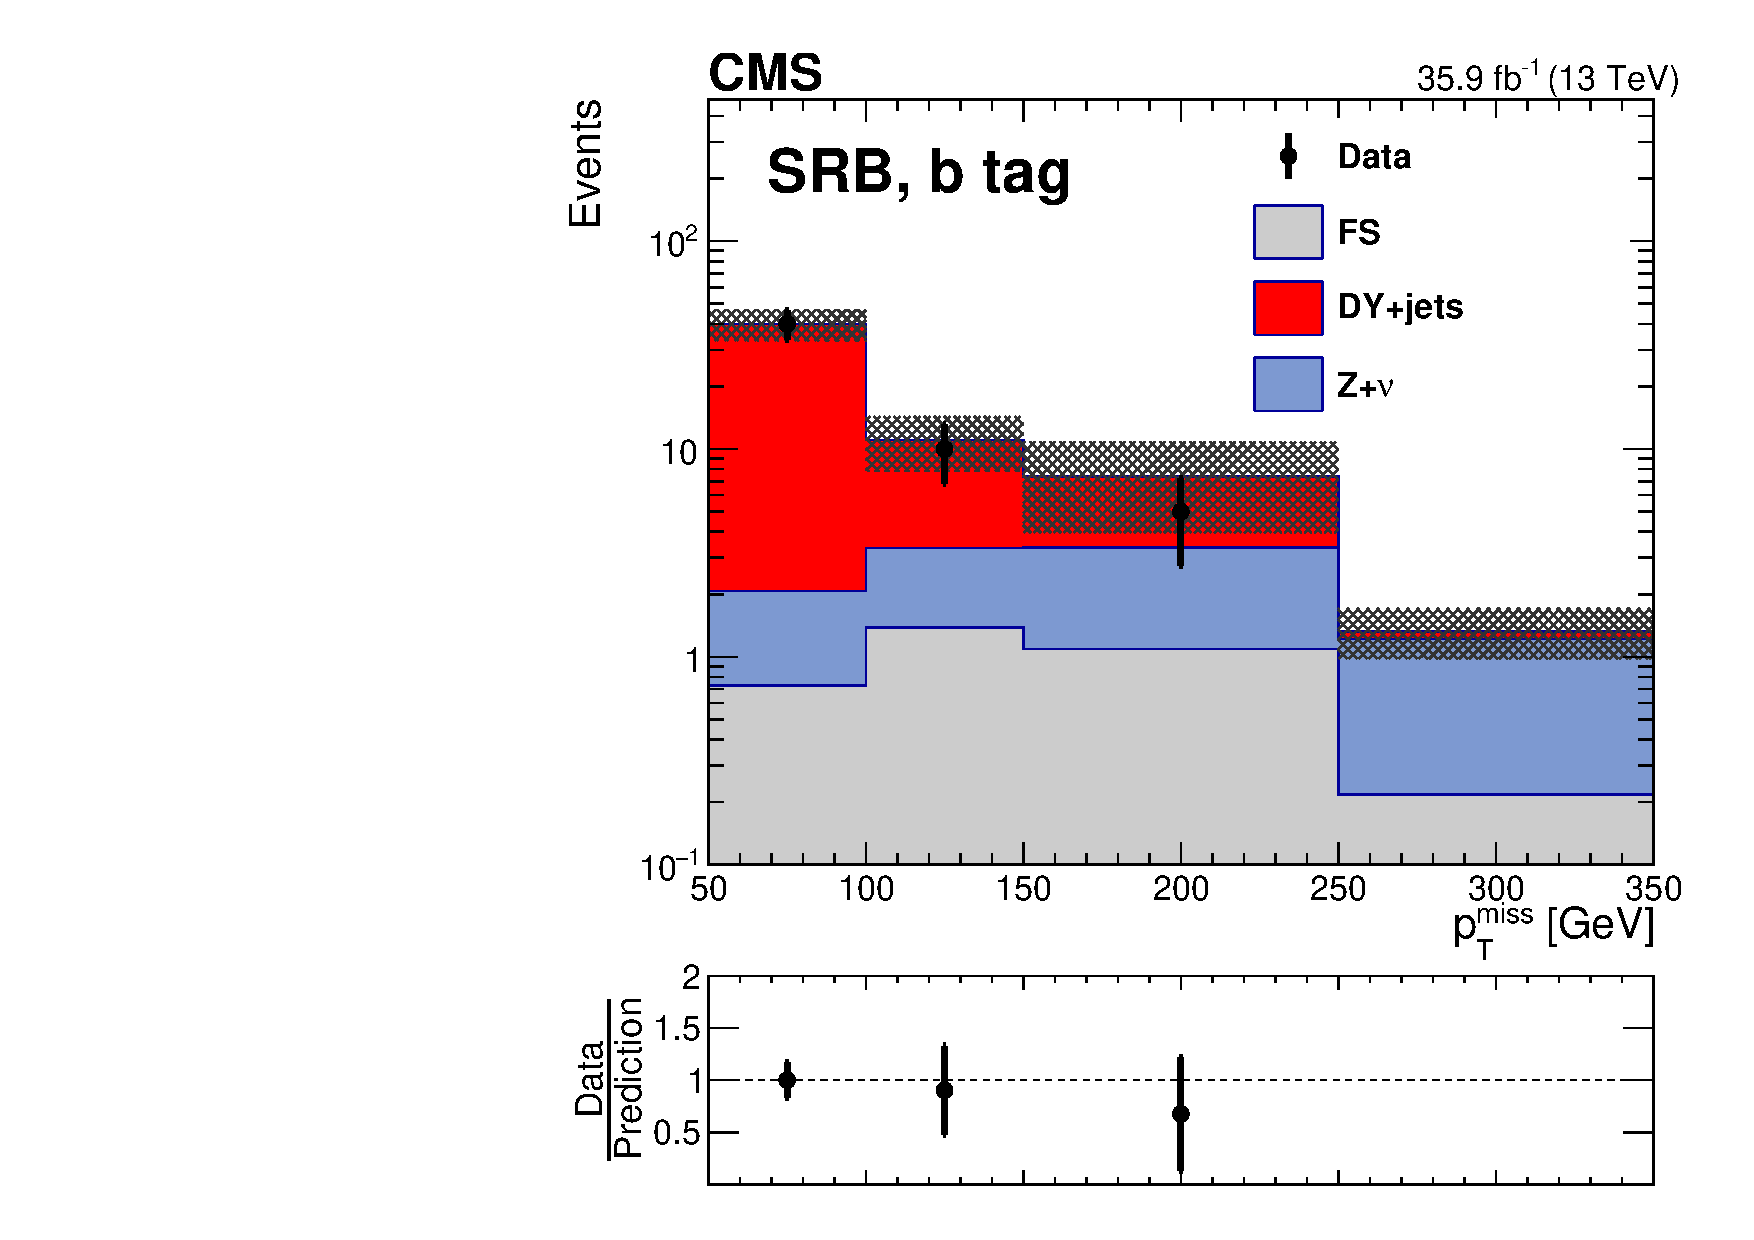
\includegraphics[width=0.35\linewidth]{figures/results/h_met_SR_4jbt.pdf}
      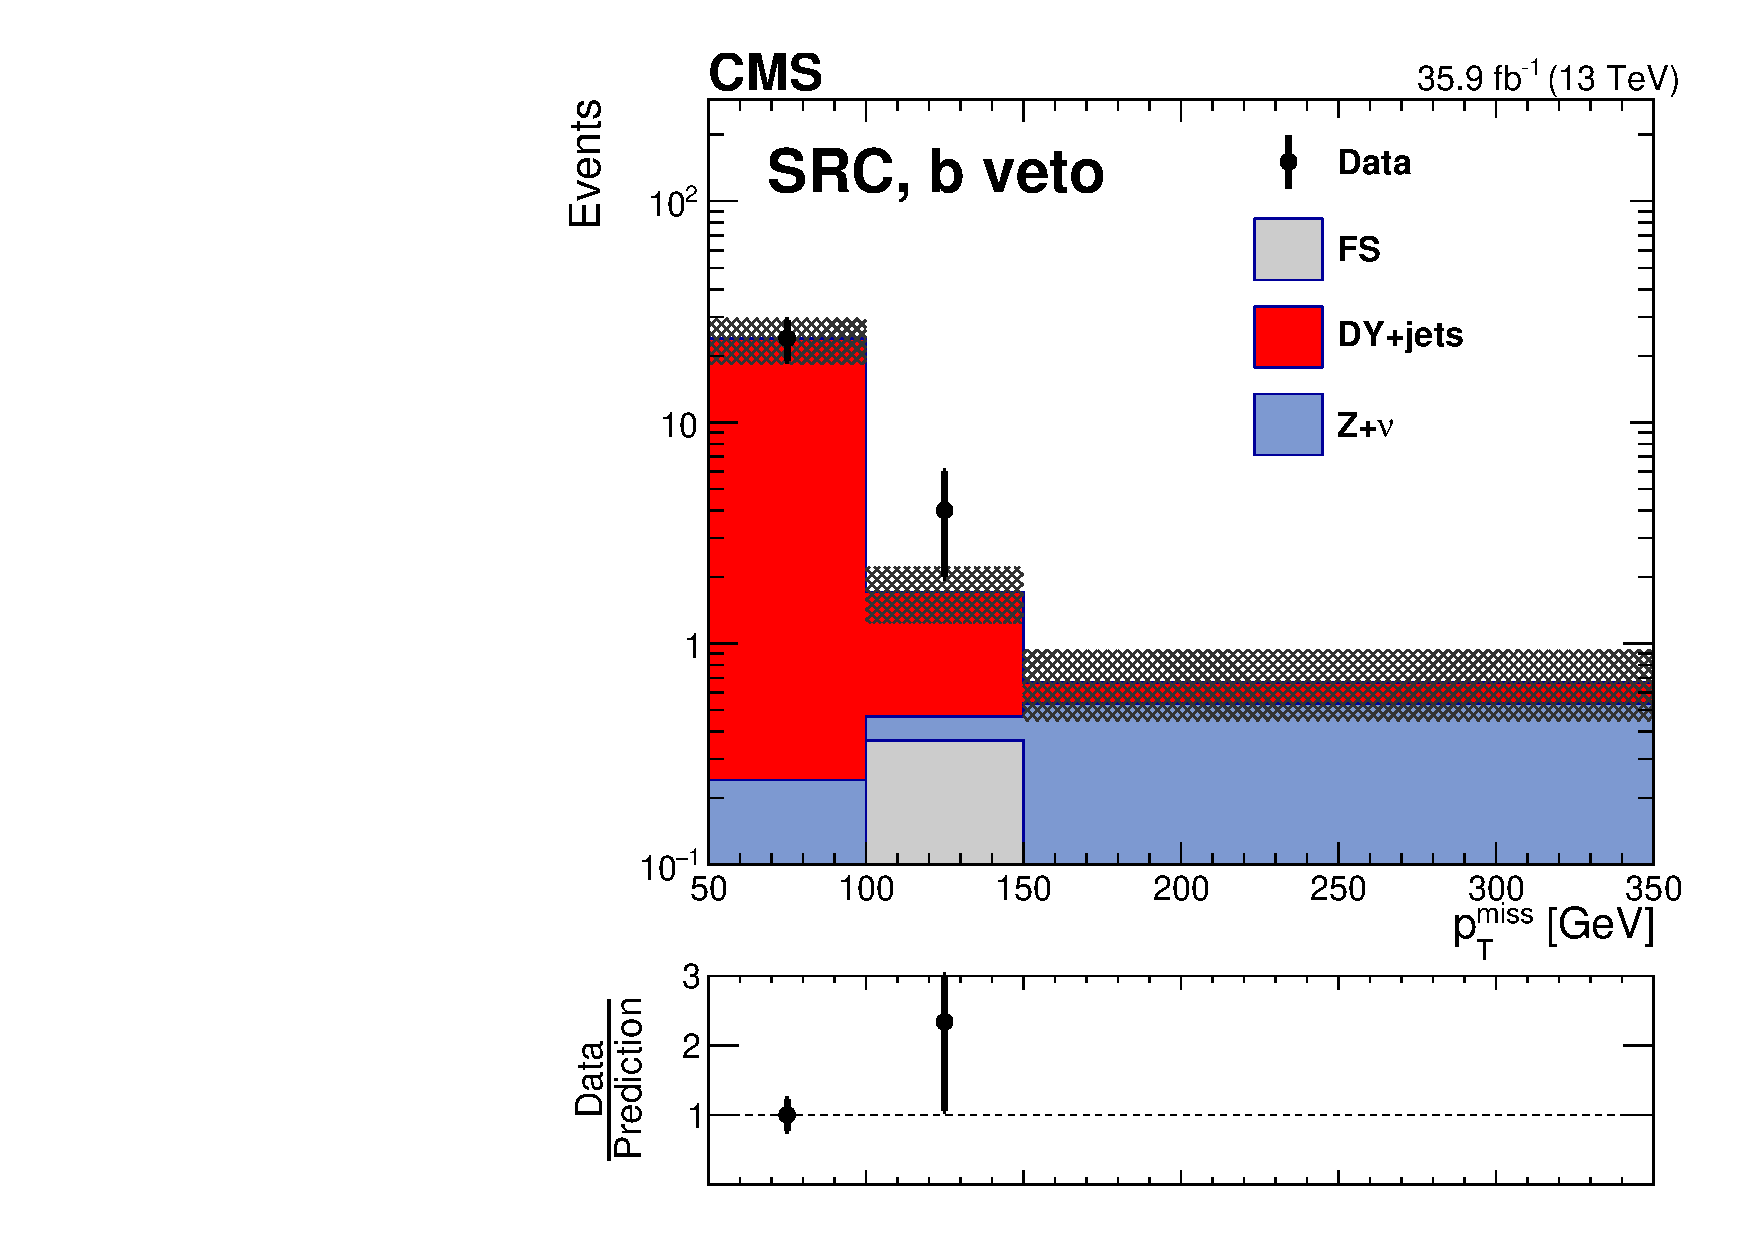
\includegraphics[width=0.35\linewidth]{figures/results/h_met_SR_6jbv.pdf}%
      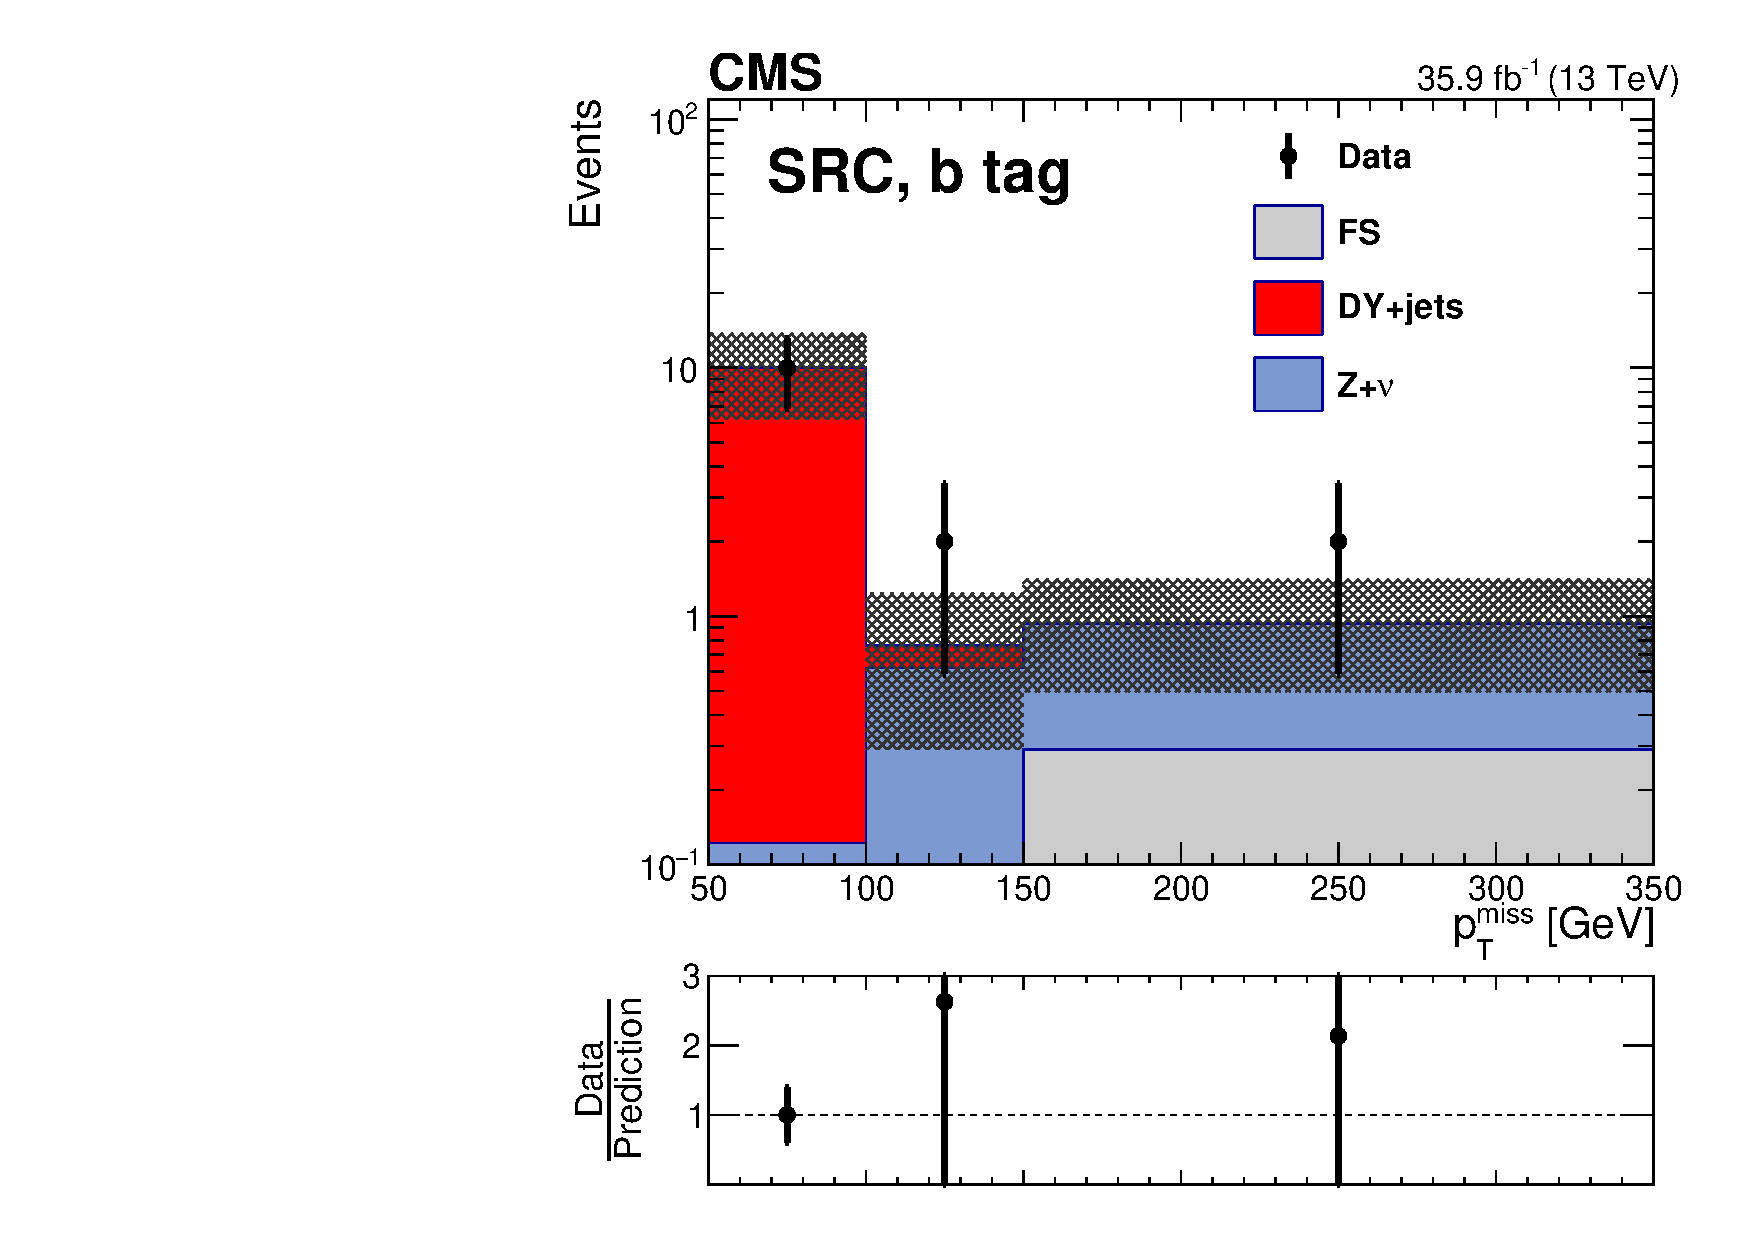
\includegraphics[width=0.35\linewidth]{figures/results/h_met_SR_6jbt.pdf}
      \caption[Results for the strong search regions are shown. The precise definitions of these regions are shown in table \ref{tab:selections_sr}.]{\label{fig:results_SR_str} Results for the strong search regions are shown. The precise definitions of these regions are shown in table \ref{tab:selections_sr}.  The black dots represent the observed counts in the signal bins, with statistical uncertainty bands shown. The colored sections represent the predictions for the labeled background, and the hatch bands represent the total systematic and statistical uncertainty for the background prediction. The uncertainty band on the ratio reflects the straightforward propagation of the uncertainties for a ratio, incorporating both the observation and background uncertainties. Note the yields in the MET 50-100 bin agree perfectly by construction as that bin is used to normalize the Z+Hadronic prediction. The numerical yields corresponding to these plots are shown in table~\ref{tab:results_SR_str}.
      }
    \end{figure}

    In the strong search regions, the data and background predictions match extremely well. Almost all bins are within the expected 1-$\sigma$ fluctuation, with the exception of the MET tail bins which have some small downward fluctuations, the largest being in SRB.

  \clearpage

  \subsection{Electroweak Search Regions}

    The following shows the results for the electroweak search regions. 

    \begin{figure}[!h]
      \centering
      \begin{tabular}{cc}
        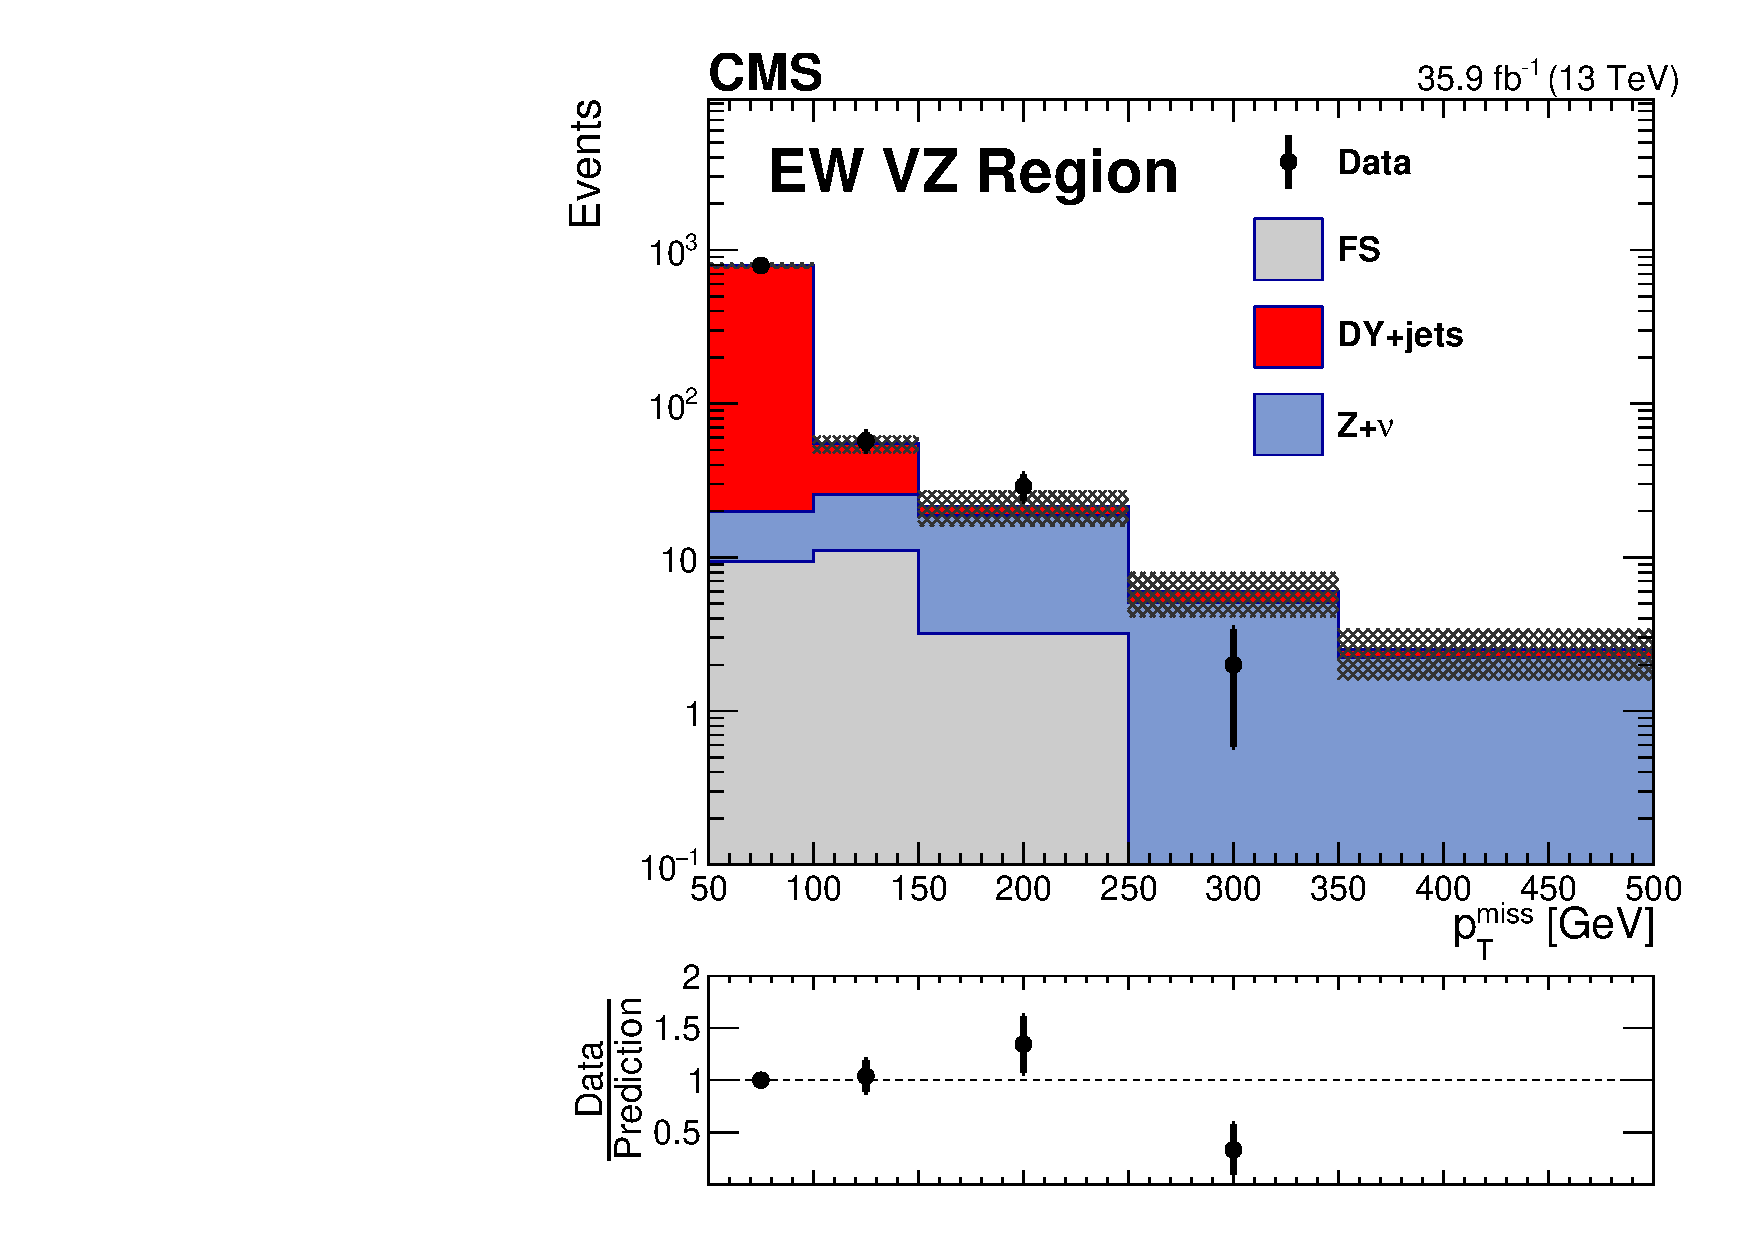
\includegraphics[width=0.4\linewidth]{figures/results/h_met_SR_tcwz.pdf} &
        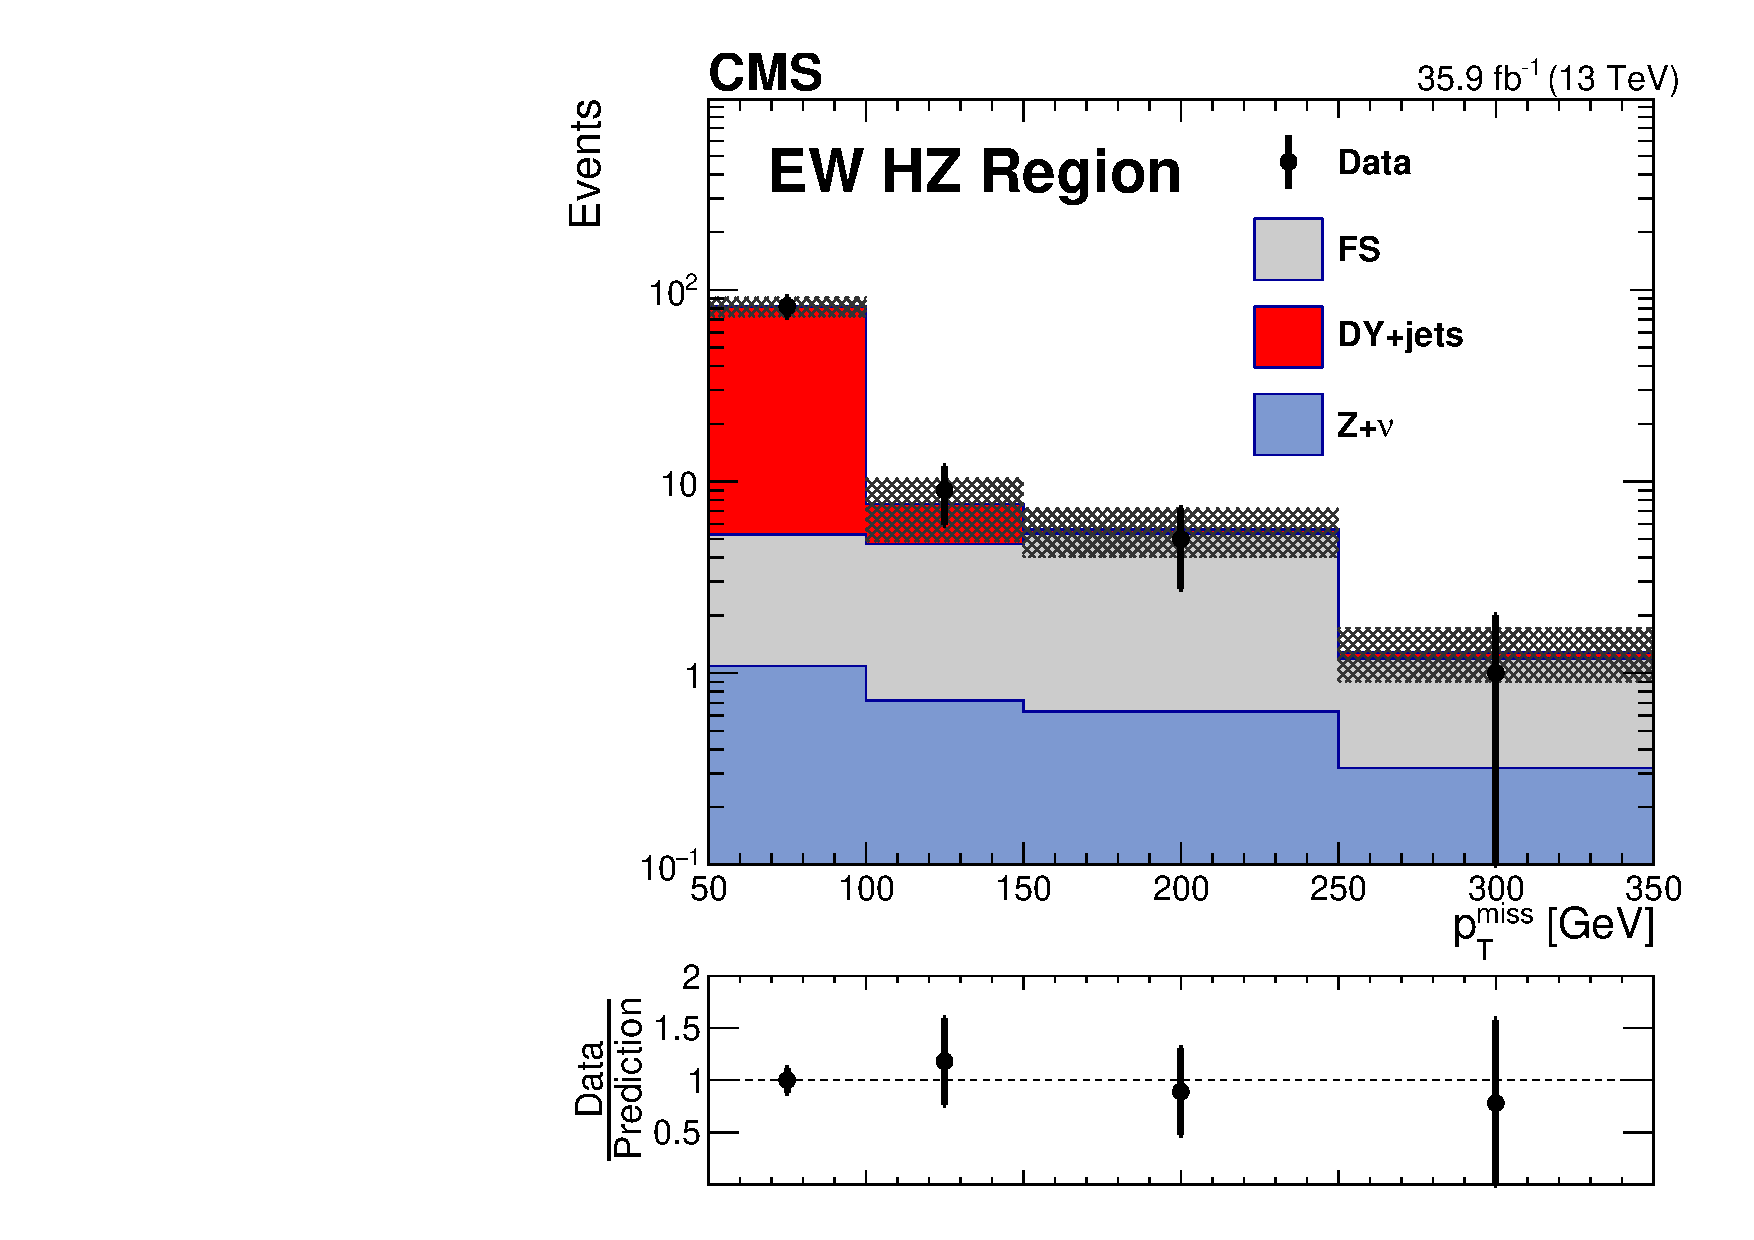
\includegraphics[width=0.4\linewidth]{figures/results/h_met_SR_tchz.pdf} \\
      \end{tabular}
      \caption[Results for the electroweak search regions are shown. The precise definitions of these regions are shown in table \ref{tab:selections_sr}.]{Results for the electroweak search regions are shown. The precise definitions of these regions are shown in table \ref{tab:selections_sr}.  The black dots represent the observed counts in the signal bins, with statistical uncertainty bands shown. The colored sections represent the predictions for the labeled background, and the hatch bands represent the total systematic and statistical uncertainty for the background prediction. The uncertainty band on the ratio reflects the straightforward propagation of the uncertainties for a ratio, incorporating both the observation and background uncertainties. Note the yields in the MET 50-100 bin agree perfectly by construction as that bin is used to normalize the Z+Hadronic prediction. The numerical yields corresponding to these plots are shown in table~\ref{tab:results_SR_ewk}. \label{fig:results_SR_ewk}
      }
    \end{figure}

    \begin{table}[!htb]
      \centering
      \caption[Numerical results for the electroweak search regions.]{\label{tab:results_SR_ewk} 
      Numerical results for the electroweak search regions are shown. The precise definitions of these regions are shown in table \ref{tab:selections_sr}. See figure~\ref{fig:results_SR_ewk}~for the corresponding plots. The agreement in the MET 50-100 bin is by construction as that bin is used to normalize the Z+Hadronic prediction. No statistically significant deviation from the standard model prediction is found.
      }
      \begin{center}
        \begin{tabular} {l | l | l | l | l | l | l }
          VZ & \MET [GeV]  & 50-100 & 100-150 & 150-250 & 250-350 & 350+ \\ \hline 
          & Z+Hadronic  & 773.2$\pm$31.9 & 29.3$\pm$4.4 & 2.9$\pm$2.1 & 1.0$\pm$0.7 & 0.3$\pm$0.3 \\
          & FS  & $9.4^{+3.0}_{-3.0}$  & $11.1^{+3.6}_{-3.6}$  & $3.2^{+1.1}_{-1.1}$  & $0.1^{+0.2}_{-0.1}$  & $0.1^{+0.2}_{-0.1}$  \\
          & Z+$\nu$  & 10.4$\pm$2.6 & 14.5$\pm$4.0 & 15.5$\pm$5.1 & 5.0$\pm$1.8 & 2.2$\pm$0.9 \\ 
          & Sum  & $793.0^{+32.2}_{-32.2}$  & $54.9^{+7.0}_{-7.0}$  & $21.6^{+5.6}_{-5.6}$  & $6.0^{+1.9}_{-1.9}$  & $2.5^{+0.9}_{-0.9}$ \\ 
          & Data  & 793 & 57 & 29 & 2 & 0 \\ \hline 


          HZ & \MET [GeV]  &  50-100 &  100-150 &  150-250 & \multicolumn{2}{l}{ 250+ } \\ \hline 
          & Z+Hadronic  &  76.7$\pm$9.4 &  2.9$\pm$2.4 &  0.3$\pm$0.2 & \multicolumn{2}{l}{ 0.1$\pm$0.1 } \\ 
          & FS  &  $4.2^{+1.4}_{-1.4}$  &  $4.0^{+1.4}_{-1.4}$  &  $4.7^{+1.6}_{-1.6}$  & \multicolumn{2}{l}{ $0.9^{+0.4}_{-0.4}$  } \\ 
          & Z+$\nu$  &  1.1$\pm$0.3 &  0.7$\pm$0.2 &  0.6$\pm$0.2 & \multicolumn{2}{l}{ 0.3$\pm$0.1 } \\ 
          & Sum  &  $82.0^{+9.5}_{-9.5}$  &  $7.6^{+2.8}_{-2.8}$  &  $5.6^{+1.6}_{-1.6}$  & \multicolumn{2}{l}{ $1.3^{+0.4}_{-0.4}$ } \\ 
          & Data  &  82 &  9 &  5 & \multicolumn{2}{l}{ 1 } \\ \hline 
        \end{tabular}
      \end{center}
    \end{table}

    The results show good agreement between the standard model background prediction and the results in data. In the HZ region, all bins are within the 1-$\sigma$ expected fluctuation. In the VZ region, a very small upward fluctuation is found in the MET 150-250 bin followed by downward fluctuations in the MET tails.

    \clearpage

\section{Signal Interpretations} \label{sec:signal_interpretations}

  As mentioned previously in \ref{sec:susy_models}, there are several simplified models we use to interpret the search results in the context of electroweak scale supersymmetry. Each signal model has a cross section for production that is set by the masses of the new particles in that model, and we assume that the addition of a process to the standard model only increases the final state counts in sensitive regions (i.e. that there is no negative interference of new physics on the relevant known physics). 

  Events are generated using physics simulation, described in \ref{sec:monte_carlo}, for an interval of \emph{mass points} in each model. Then the compatibility of the observed data are considered under the null-hypothesis and under the hypothesis that the signal model is present in nature. A confidence level is set us using the CL$_s$ method described in \cite{CLS_method}, the details of which are outlined in the next section.

  \subsection{Statistical Treatment} \label{sec:statistical_treatment}
    This analysis uses the CMS Higgs Combine Tool \cite{higgs_combine} to produce our confidence intervals. A brief description of the statistical methods used are presented in this section, more detail can be found in \cite{higgs_combine}, \cite{Likelihood_Cowen_Cranmer}, and \cite{CLS_method}. 

    In any given search bin, a prediction is made for the expected standard model background as described in \ref{sec:background_estimation_methods}. Each prediction method is characterized by several largely uncorrelated sources of uncertainty, called \emph{nuisance parameters}, whose one $\sigma$ uncertainty bands are combined in quadrature to give a one $\sigma$ band for the background prediction. The set of all such parameters in this analysis is denoted by $\vec{\theta}$. Each nuisance is modeled as a random variable that multiplies the relevant prediction. The distribution from which this random variable is assumed to be sampled is shown in table \ref{tab:systematic_shapes} for every nuisance in this analysis.\footnote{Further details about the uncertainty sources considered for the background predictions can be found in \ref{sec:background_estimation_methods}, and for the signal model prediction in \ref{sec:systematics_in_signal_yield}.}

    \subsubsection{The Likelihood of an Observation}

      The data in any signal bin can be seen as being sampled from a Poisson distribution. Since each search region is independent, the likelihood of observing the results we've seen in data is the product of the likelihoods to see the outcome in each search bin:

      \begin{align} 
        \mathcal{L}(\text{observation}) = \prod_{i \in \text{Search Bin}} \frac{\lambda_i^{n_i} e^{-\lambda_i}}{n_i !}. \label{eq:niave_likelihood}
      \end{align}

      where each $\lambda_i$ and $n_i$ are the expected and observed number of events in search bin $i$ respectively. If the signal does not exists in nature (the background only hypothesis), then $\lambda_i = b$, the background prediction for the bin. If the signal does exist in nature then $\lambda_i = s + b$, the sum of the signal and background predictions\footnote{again, we assume no negative interference}. However, due to the probabilistic nature of the background and signal predictions, $\lambda$ itself must be modeled by a distribution of possible values. 

      \[
        \lambda_i(\vec{\theta}, \mu) = \mu s(\vec{\theta}) + b(\vec{\theta}).
      \]

      We've also added the \emph{signal strength} $\mu$ to the definition of $\lambda$ for later mathematical convenience. $\mu$ is a parameter that allows us to interpolate any further mathematical constructions between the signal+background and null hypothesis by varying from 1 to 0.

      The nuisance parameters are chosen such that they act as multiplicative factors on the prediction value, that is to say for $K$ relevant nuisance parameters\footnote{Not all nuisance parameters effect every prediction. For instance, if $b$ were the prediction of the Z+Hadronic background in SRA, there would be 4 multiplicative factors listed in table \ref{tab:systematic_shapes}} and a central value denoted by $\widetilde{b}$,

      \[
        b(\theta) = \widetilde{b} \times \theta^0 \times ... \times \theta^K,
      \]

      and the same relationship holds for $s(\theta)$. The probability that a nuisance parameter takes a specific value is drawn from a probability distribution that was fit to auxiliary measurements designed to capture the expected variation of the nuisance. The distribution chosen for each nuisance used in this analysis is given in table \ref{tab:systematic_shapes}. 

      Taking into account the probabilistic nature of $\lambda(\vec{\theta}, \mu)$, the likelihood in eq \ref{eq:niave_likelihood} should be updated with a multiplicative factor that accounts for the probability of certain set of values for $\vec{\theta}$. The likelihood that we observe our data given a specific nuisance configuration and signal strength $\mu$

      \begin{equation} 
        \mathcal{L}(\text{observation} | \vec{\theta}, \mu ) = P(\vec{\theta}) \left( \prod_{i \in \text{Search Bin}} \frac{\lambda_i(\vec{\theta}, \mu)^{n_i} e^{-\lambda_i(\vec{\theta}, \mu)}}{n_i !} \right), \label{eq:true_likelihood}
      \end{equation}
      

      where $P(\vec{a})$ is the probability that the nuisance vector has the value $\vec{a}$. Given that we assume the nuisances are completely uncorrelated, $P(\vec{\theta})$ will be a product of terms for each nuisance with distributions chosen from table \ref{tab:systematic_shapes}. As an example, if the only nuisances considered were the luminosity and the closure for the low \MET bin of the SRA Z+Hadronic prediction, where the value of the luminosity multiplicative factor is denoted by $\theta[0]$ and the closure factor is denoted by $\theta[1]$, the full likelihood function for the GMSB signal model would read

      \begin{multline}
          \mathcal{L}(\vec{\theta}, \mu | \text{data} ) = \\
          \underbrace{\frac{1}{\sqrt{2\pi} \ln(1.026)} e^{-\frac{\left(\ln\theta[0]\right)^2}{2 \left(\ln 1.026\right)^2}} \frac{1}{\theta[0]}}_{\text{Log Normal Distribution for Luminosity}} \times \underbrace{\frac{1}{\sqrt{2\pi} \ln(1.2)} e^{-\frac{\left(\ln\theta[1]\right)^2}{2 \left(\ln 1.2\right)^2}} \frac{1}{\theta[1]}}_{\text{Log Normal Distribution for SRA Low \MET Closure}} \times \\
          \underbrace{\frac{\lambda_i(\vec{\theta}, \mu)^{n_{\text{SRA}}} e^{-\lambda_i(\vec{\theta}, \mu)}}{n_{\text{SRA}} !}}_{\text{Poisson Distribution for SRA Bin Count}} \times ... \times \underbrace{\frac{\lambda_i(\vec{\theta}, \mu)^{n_{\text{SRCb}}} e^{-\lambda_i(\vec{\theta}, \mu)}}{n_{\text{SRCb}} !}}_{\text{Only the 6 Strong Search Regions Contribute}}
      \end{multline}


      \begin{table}[!h]
        \begin{center}
          \caption{\label{tab:systematic_shapes} Systematic Uncertainty Assumed Shapes. }
          \begin{tabular}{l | l | l}
            \hline
            \hline
            Prediction  & Nuisance  & Distribution \\
            \hline
            \textbf{Z + Hadronic}     & Closure                    & log Normal \\
                                      & EWK Subtraction            & log Normal \\
                                      & $\gamma$ Normalization     & log Normal \\
                                      & $\gamma$ Statistics        & log Normal \\
            \hline
            \textbf{Flavor Symmetric} & $\kappa$ Value             & log Normal \\
                                      & \rsfof Value               & log Normal \\
                                      & Same Sign Statistics       & $\Gamma$   \\
            \hline
            \textbf{Z + $\nu$}        & Closure                    & log Normal \\
                                      & MC Statistics              & log Normal \\
            \hline
            \textbf{Signal}           & MC Statistics              & log Normal \\
                                      & B-tag eff, heavy flavor    & log Normal \\
                                      & B-tag eff, light flavor    & log Normal \\
                                      & Jet Energy Scale           & log Normal \\
                                      & Lepton Trigger Efficiency  & log Normal \\
                                      & Lepton ID/Iso Efficiency   & log Normal \\
                                      & ISR Modeling               & log Normal \\
                                      & Luminosity                 & log Normal \\
                                      & Fastsim MET Modeling       & log Normal \\
                                      & Generator Scale variations & log Normal \\
                                      & PU reweighting             & log Normal \\
            \hline
            \hline
          \end{tabular}
        \end{center}
      \end{table}

      The nuisances for the background predictions were described in the previous chapter, a breif description of the signal nuisances is given in section \ref{sec:systematics_in_signal_yield}.
    \subsubsection{Setting Exclusion Limits} \label{sec:setting_exclusion_limits}

      In order to exclude a mass point for a signal model, we adopt the CL$_s$ method. The basic premise is that in order for a mass point to be excluded at the 95\% confidence level, we require that, under some metric of probability, the background only hypothesis is 20 times more likely than the signal+background hypothesis\footnote{$\frac{1}{20}$ being the left of 5\% from 95\%}.

      The metric of probability we use is based upon the following formalism: 

      First, we construct the so-called profile-likelihood ratio, a ``test statistic" defined as

      \begin{align} \label{eq:profile_log_likelihood}
        q_\mu = -2 \ln \left( \frac{\mathcal{L}(\text{observation} | \vec{\theta}_{\mu}, \mu)}{\mathcal{L}(\text{observation} | \vec{\theta}_{\hat{\mu}}, \hat{\mu})} \right)
      \end{align}

      where

      \begin{align*}
        \vec{\theta}_a &= \vec{\theta} \text{ such that } \mathcal{L}(\text{observation} | \vec{\theta}, a) \text{ is maximal, and } \\
        \hat{\mu} &= \mu \text{ such that } \mathcal{L}(\text{observation} | \vec{\theta}_\mu, \mu) \text{ is maximal. \footnotemark{} }
      \end{align*}
      \footnotetext{This means that $\mathcal{L}(\text{observation} | \vec{\theta}_{\hat{\mu}} ,\hat{\mu} )$ is the global maximum of the likelihood}
      
       In the above, we only search over values of $\hat{\mu} \le \mu$, if the the global maximum is found outside this region, $q_\mu$ is set to 0. The denominator in eq \ref{eq:profile_log_likelihood} is the global maximum of the likelihood function over all values of $\vec{\theta}$ and $\mu$, where $\mu$ is less than the $\mu$ in the numerator. The numerator in eq \ref{eq:profile_log_likelihood} is the maximum likelihood of the observed data over all possible $\theta$ configurations, but for a fixed $\mu$. If a value of $\mu$ is very likely, then we expect the $\theta$ parameter to ensure that correlations between bins are not double counted in their effect on the compatibility of the observation. For instance, if the luminosity measurement was 3\% low for our dataset and no new physics exists, the hope is that $\theta_0$ will have the luminosity factor of 1.03.

       Notice that $q_\mu$ is bounded by 0 below and unbounded above. If an observation point is highly likely w.r.t the global maximum, then $q_\mu$ is 0. To define the 95\% confidence interval, it is easiest to think in terms of simulated data. \footnote{ although in practice analytic approximations are made in order to do the following calculations} 

       Let $q^\text{obs}_\mu$ be the value of $q$ for some $\mu$ given the actual results of our experiment shown in \ref{sec:results}. We construct a distribution of the possible values for $q_\mu$ under the null hypothesis by using the likelihood in eq. \ref{eq:true_likelihood} to give simulated results for an ensemble experiments and compute $q_\mu$ for each simulated result. We assume the distribution of $q_\mu$ to tend larger for larger values of $\mu$ since the probability of measuring a new physics process should decrease with the processes cross section in the null hypothesis, and high values of $q$ are associated with unlikely data. The percentage of simulated experiments where $q_\mu$ is larger than $q^\text{obs}_0$ is called CL$_b$, the ``confidence level" of the background only hypothesis. In short, we compute the percentage of experiments that give a less likely outcome than what we found. 

       We repeat this procedure again, only in this case using the background+signal hypothesis to generate our simulated experiments, i.e. $\mu$ is not required to be 0 in $\lambda$. The percentage of simulated experiments where $q_\mu$ is larger than $q^\text{obs}_\mu$ is called CL$_{s+b}$, the ``confidence level" of the signal+background hypothesis. 

       Finally, the value of $\mu$ for which 

       \[
        \text{CL}_s = \frac{\text{CL}_{s+b}}{\text{CL}_b} \le 0.05
       \]

       is called the exclusion limit for the mass point. If the value of $\mu$ for which this condition is met is 1 or more, the mass point can not be excluded at the 95\% level. If the value of $\mu$ is less than 1, then we call the mass point excluded.

       In the final exclusion plots, an ``expected limit" is normally drawn as well. To construct this limit, we follow the same limit setting procedure described above, but replace $q^\text{obs}_\mu$ with the $q$ value for a simulated result of our experiment assuming the background only hypothesis. This process is then repeated to produce a distribution of excluded $\mu$ values. The central value and one-$\sigma$ expected limits are then taken from this distribution.

  \subsection{Systematics in Signal Yield} \label{sec:systematics_in_signal_yield}
    In order to interpret these results in the context of electroweak scale SUSY, the simplified SUSY models in figure \ref{fig:feynman_str} and \ref{fig:feynman_ewk} are simulated using the madgraph package as explained in sec \ref{sec:monte_carlo}. The simulated events are then run through the same software used to reconstruct and select real data events. 

    Table \ref{tab:syst} is a list of nuisance parameters associated with the simulation of SUSY models. Although many of these could also be applied to the other simulated background predictions, to wit: the Z+$\nu$ background, other nuisances would dominate these mostly few-percentage level effects.\footnote{Fastsim \MET modeling is unique to the SUSY simulation and statistics vary by sample.} 

    \begin{table}[htb]
      \begin{center}
        \caption{\label{tab:syst} Systematic uncertainties of the expected signal yield. }
        \begin{tabular}{l|c}
          \hline
          \hline
          Source                     & Value (\%) \\
          \hline
          MC Statistics              & $\pm$1--60 \\
          B-tag eff, heavy flavor    & $\pm$3     \\
          B-tag eff, light flavor    & $\pm$2     \\
          Jet Energy Scale           & $\pm$1--15 \\
          Lepton Trigger Efficiency  & $\pm$3     \\
          Lepton ID/Iso Efficiency   & $\pm$7     \\
          ISR Modeling               & $\pm$0--7  \\
          Luminosity \cite{Lumi_unc} & $\pm$2.6   \\
          Fastsim MET Modeling       & $\pm$1--60 \\
          Generator Scale variations & $\pm$3     \\
          PU reweighting             & $\pm$3     \\
          \hline
          Total uncertainty on signal& $\pm$10--60 \\
          \hline
          \hline
        \end{tabular}
      \end{center}
    \end{table}

    A brief description of the nuisances follows: The MC statistics uncertainty is the statistical uncertainty on number of signal events generated. The B-tag efficiency for heavy (light) flavor jets characterizes the difference between MC and data jet reconstruction for jets originating from bottom and charm (up, down, and strange) quarks. The jet energy scale nuisance is due to the uncertainty on the correction applied to jet energies. The lepton efficiencies are due to the simulated modeling of the acceptance of leptons. The ISR modeling is due to uncertainty in modeling the initial state radiation in simulation. The luminosity nuisance is due to uncertainty in the amount of luminosity provided to the CMS detector. The Fastsim MET modeling is due to the lower quality fast simulation of the CMS detector used for signal simulation, and its effect on the MET resolution. The generator scale variations characterize the uncertainty in QFT parameters, like the proton pdfs, when computing matrix elements. Finally, the pileup reweighting nuisance is due to the uncertainty in amount of pileup added to signal events.

  \subsection{Exclusion Limits} \label{sec:exclusion_limits}

    In this section, the results in \ref{sec:results} are interpreted in the context of the simplified supersymmetric models described in \ref{sec:susy_models}. For the sake of convenience, the Feynman diagrams for these models are reproduced in figure \ref{fig:SUSY_diagrams_interpretation_sec}.

    \begin{figure}[!h]
      \centering
      \begin{subfigure}[b]{0.49\textwidth}
        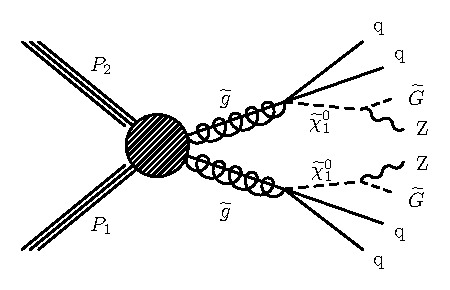
\includegraphics[width=\textwidth]{figures/diagrams/T5ZZ.pdf} 
        \caption{Strong GMSB SUSY}
        \label{fig:t5zz_diagram_interpretations}
      \end{subfigure}
      \begin{subfigure}[b]{0.49\textwidth}
        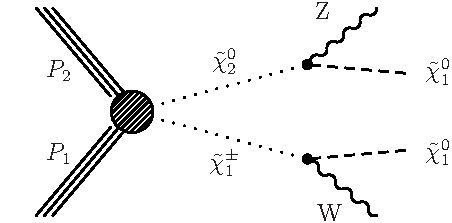
\includegraphics[width=\textwidth]{figures/diagrams/TChiWZ.pdf}
        \caption{EWK SUSY With WZ Production}
        \label{fig:tchiwz_diagram_interpretations}
      \end{subfigure} \\
      \begin{subfigure}[b]{0.49\textwidth}
        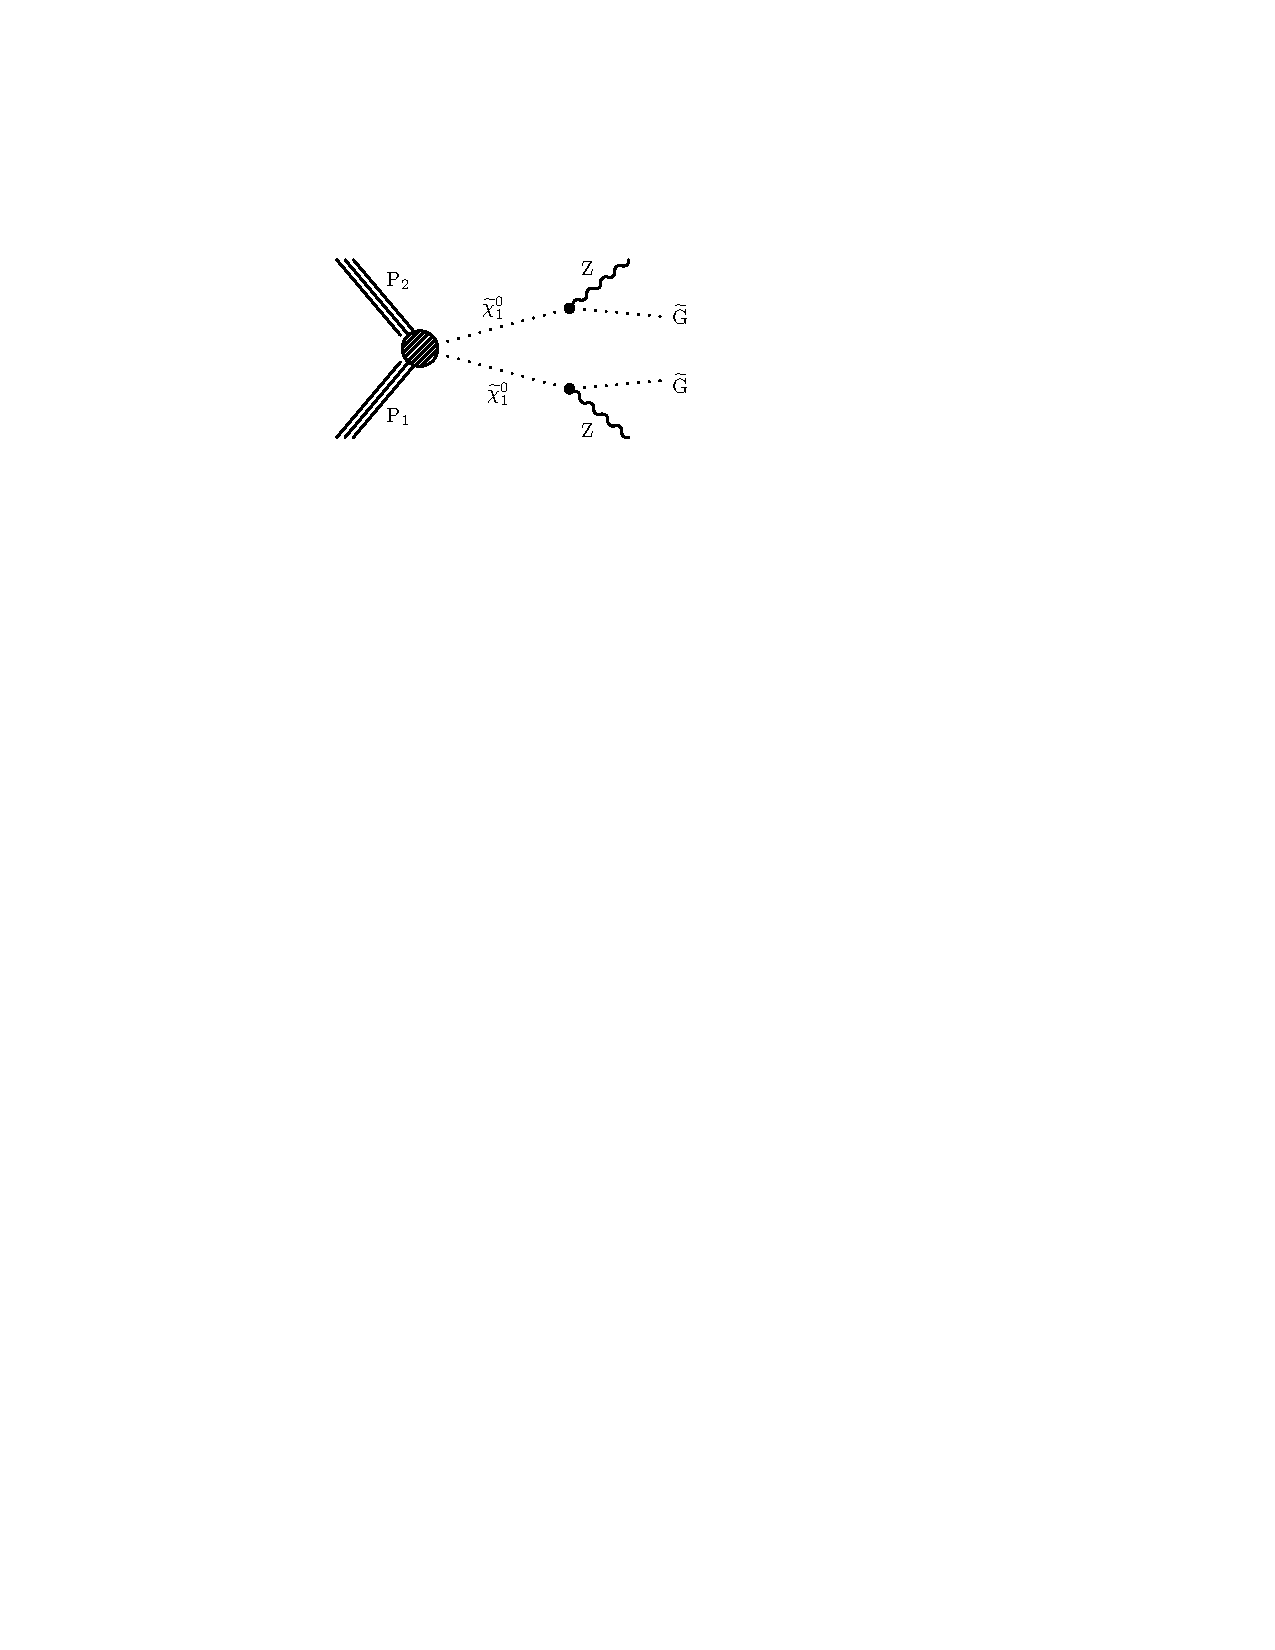
\includegraphics[width=\textwidth]{figures/diagrams/TChiZZ.pdf}
        \caption{EWK SUSY With ZZ Production}
        \label{fig:tchizz_diagram_interpretations}
      \end{subfigure}
      \begin{subfigure}[b]{0.49\textwidth}
        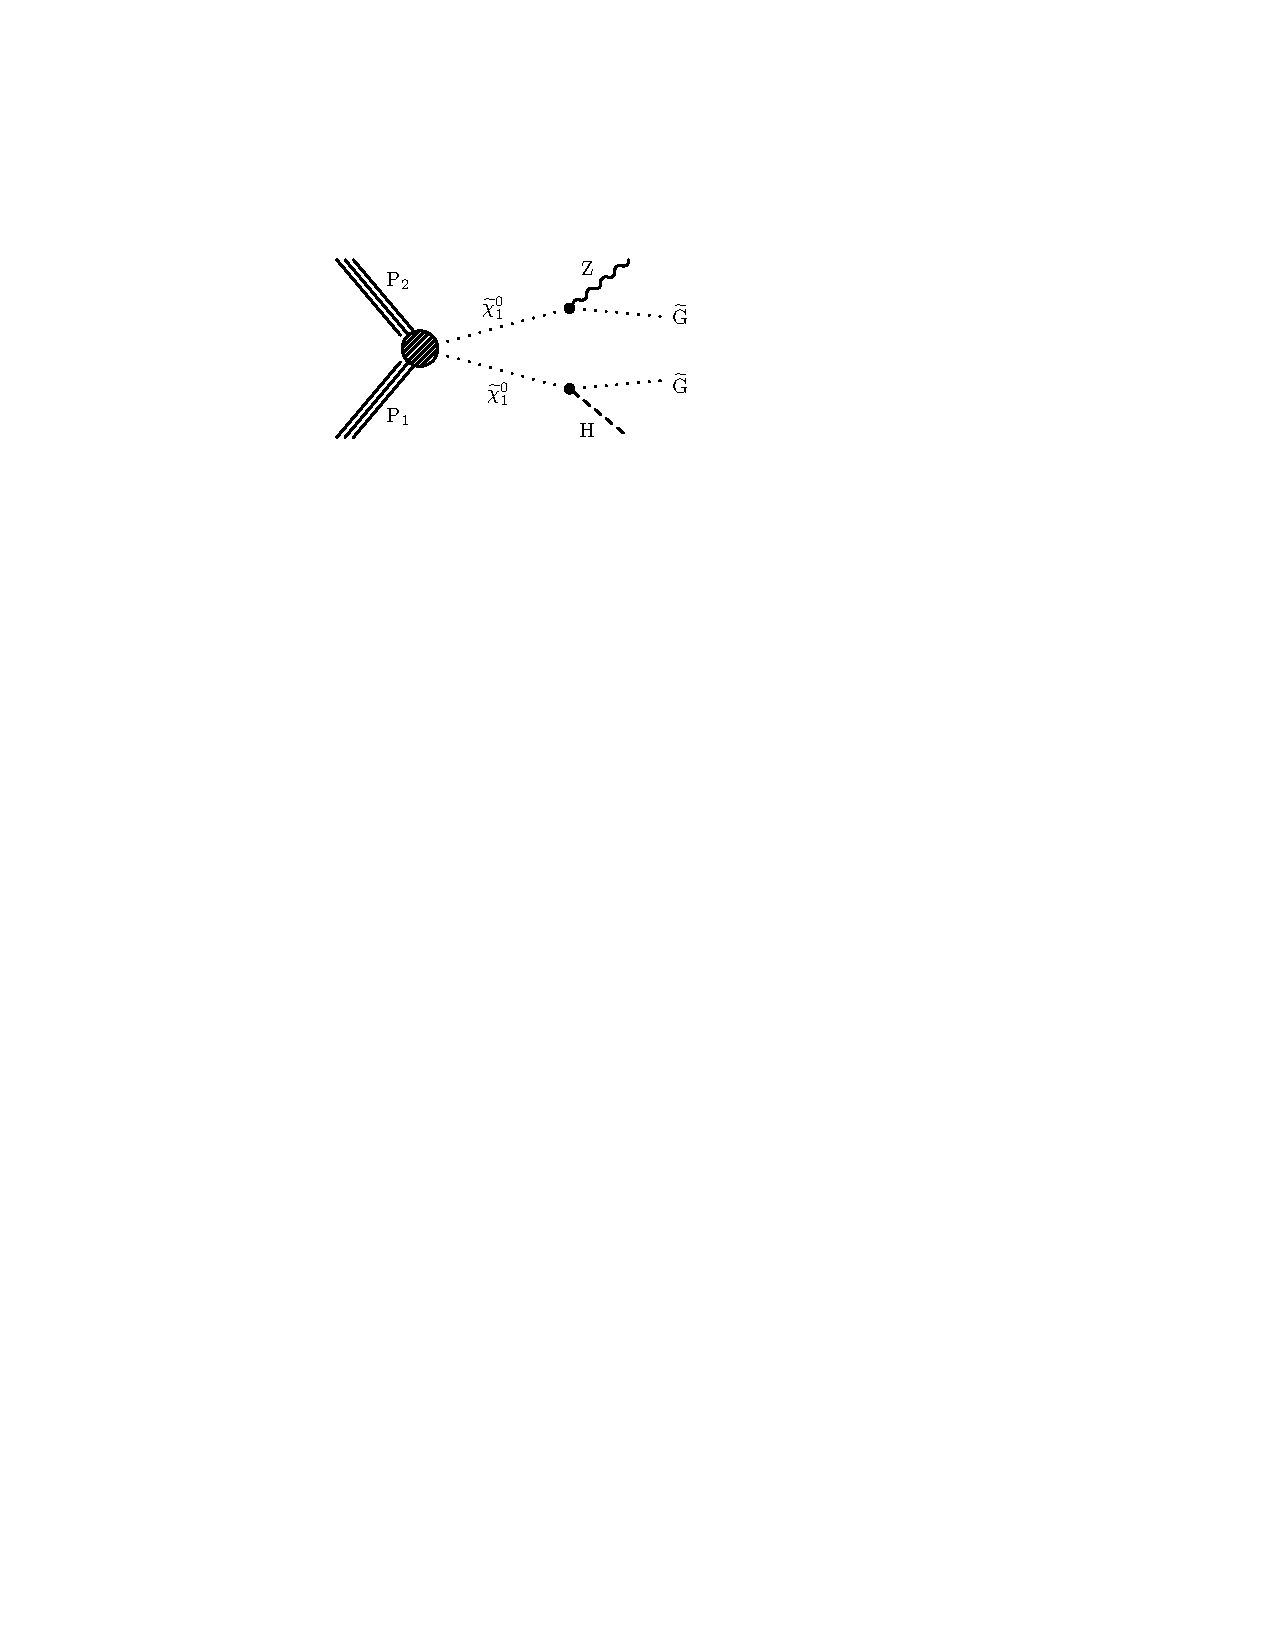
\includegraphics[width=\textwidth]{figures/diagrams/TChiHZ.pdf}
        \caption{EWK SUSY With HZ Production}
        \label{fig:tchihz_diagram_interpretations}
      \end{subfigure}
      \caption{ \label{fig:SUSY_diagrams_interpretation_sec}
        Feynman diagrams for the SUSY models used in interpreting the results of this analysis. More exposition on the properties of these models is found in sec \ref{sec:susy_models}.}
    \end{figure}

    For the strong production model, shown in fig. \ref{fig:t5zz_diagram_interpretations}, the exclusion limits are shown in figure \ref{fig:t5zz_interpretation}, which combines data from all the strong search regions in the likelihood function. The free parameters in this model are the gluino and $\widetilde{\chi}^0_1$ masses, the gravitino mass is set to 1 GeV. The bulk of the sensitivity comes from the high jet multiplicity and high \MET search regions, SRB(b) and SRC(b). Due to the downward fluctuations in most of the high \MET bins, our observed limit is slightly better than the expected limit. In a previous CMS result probing similar final states,\cite{paper_2016} this simplified model was excluded at the 95\% CL for gluino masses roughly below 1.2-1.3 TeV for $\widetilde{\chi}^0_1$ masses below 1 TeV. This analysis advances the limits significantly, by roughly 400 GeV in gluino mass for similar $\widetilde{\chi}^0_1$ masses, as can be seen in figure \ref{fig:t5zz_interpretation}. 

    In the compressed spectrum (where the $\widetilde{\chi}^0_1$ mass is close to the gluino mass), the neutralino is expected to carry away more energy from the gluino than the quarks. In the extremely compressed regions where the $\widetilde{\chi}^0_1$ and gluino masses are only separated by about 100 GeV, it's possible that one of the jets can be missed. This makes SRB/SRBb more important regions at the top of the plot. The data shows a downward fluctuation in the high \MET bins of those regions, and so the observed limits tend to move towards higher masses than the expected limits. At large mass splittings, i.e. points near the x axis, SRC and SRCb are the most important regions due to the high jet multiplicity. There is a small upwards fluctuation in SRCb which offsets the downward fluctuations in SRB, SRBb, and SRC; this causes the observed limit to be closer to the expected limit in the bottom of the plot.

    \begin{figure}[!h]
      \centering
        \begin{subfigure}[b]{0.4\textwidth}
          \label{fig:t5zz_interpretations_2015}
          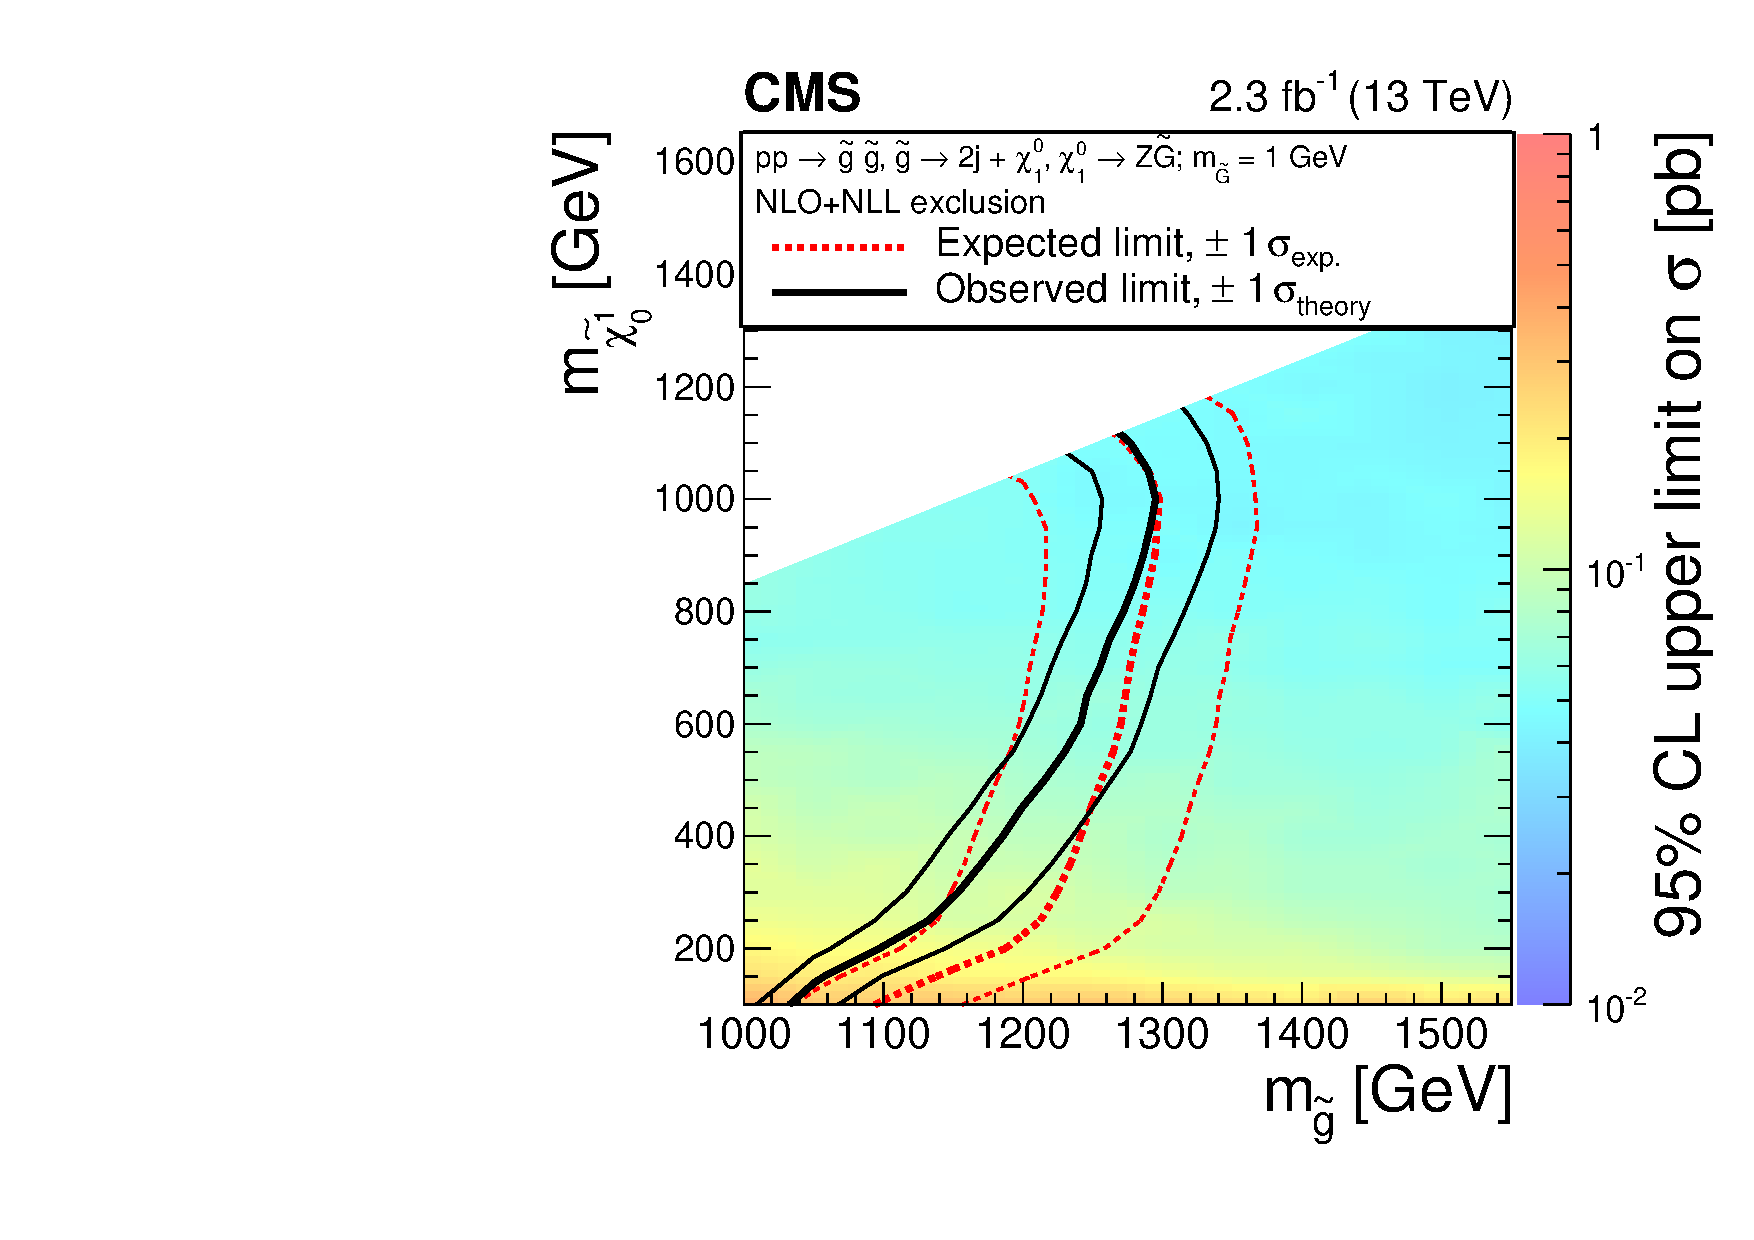
\includegraphics[width=\textwidth]{figures/interpretations/t5zz_2015_exclusion.pdf}
          \caption{Previous best limits on this model}
        \end{subfigure}
        \begin{subfigure}[b]{0.4\textwidth}
          \label{fig:t5zz_interpretations_current}
          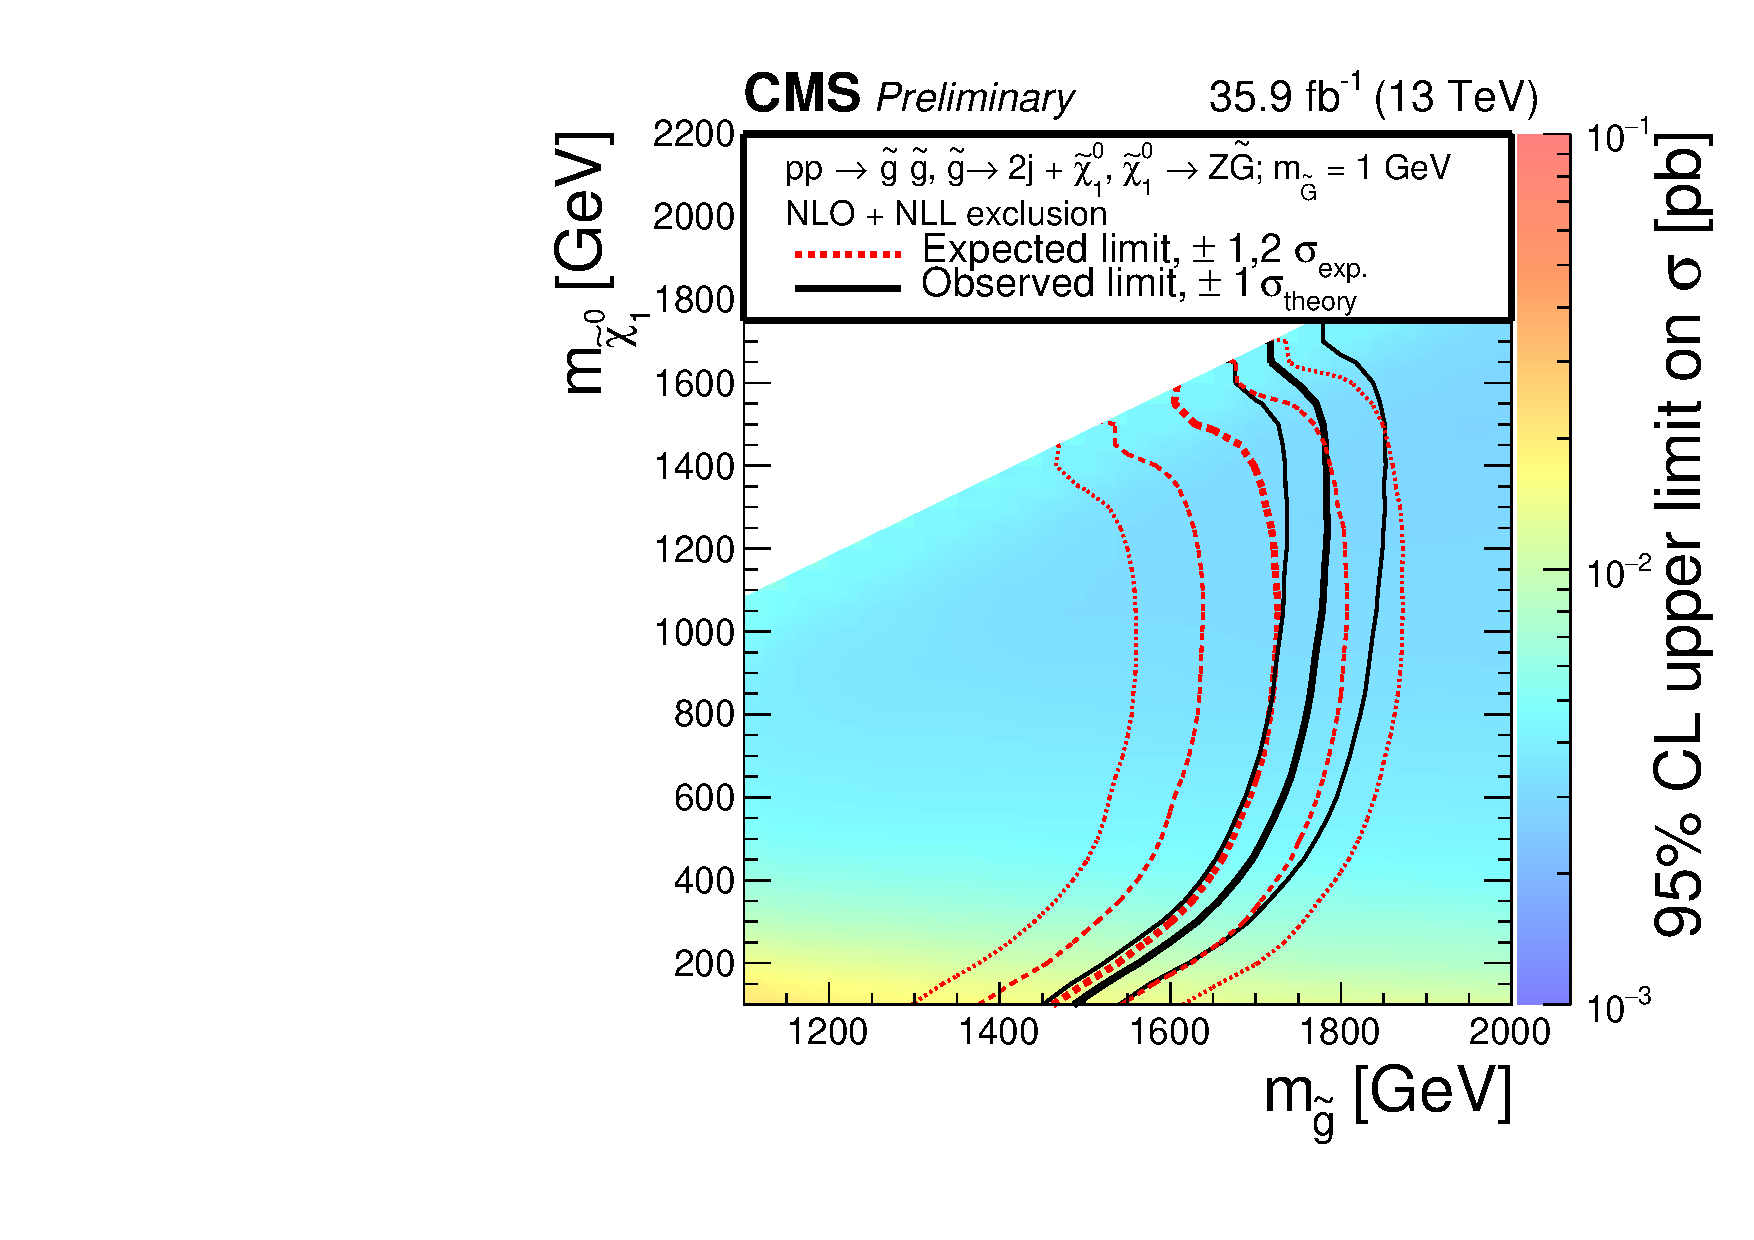
\includegraphics[width=\textwidth]{figures/interpretations/T5ZZ_Exclusion_13TeV.pdf}
          \caption{Limits set by this analysis}
        \end{subfigure}
      \caption[The limits set on the strong GMSB SUSY model.]{ \label{fig:t5zz_interpretation}
        The limits set on the strong GMSB SUSY model from fig. \ref{fig:t5zz_diagram_interpretations} are shown to the right. To the left, we show the previous best limit on this model set by CMS in 2016.\cite{paper_2016} The solid black and bold dotted red lines trace out the largest masses where the signal strength $\mu$ is less than 1 at 95\% confidence for observed and expected data respectively as described in section \ref{sec:setting_exclusion_limits}, mass points to the left of these line are excluded. The data excludes this model at the 95\% CL for gluino masses below 1450 GeV for low LSP masses, and below 1750 GeV for large LSP masses.
      }
    \end{figure}

    Figure \ref{fig:tchiwz_interpretation} shows the exclusion limits for the electroweak WZ model in fig. \ref{fig:tchiwz_diagram_interpretations}. For this model, data from the electroweak regions are used in the likelihood, however almost all the discriminatory power comes from the VZ region. The free parameters in this model are the mass of the $\widetilde{\chi}^0_1$ and $\widetilde{\chi}^{\pm}_1$, the $\widetilde{\chi}^0_2$ mass is set equal to that of the $\widetilde{\chi}^{\pm}_1$. Downward fluctuations in the high \MET bins for that region again make the observed limits stronger than the expected limits. For light LSP mass points, the model is excluded for $\widetilde{\chi}^{\pm}_1$ and $\widetilde{\chi}^0_2$ masses up to 600 GeV, better than double the previous limits. In the high $\widetilde{\chi}^{\pm}_1$ and $\widetilde{\chi}^0_2$ mass range, the excluded LSP mass range extends to around 250 GeV. 

    \begin{figure}[!h]
      \centering
        \begin{subfigure}[b]{0.4\textwidth}
          \label{fig:t5zz_interpretations_2015}
          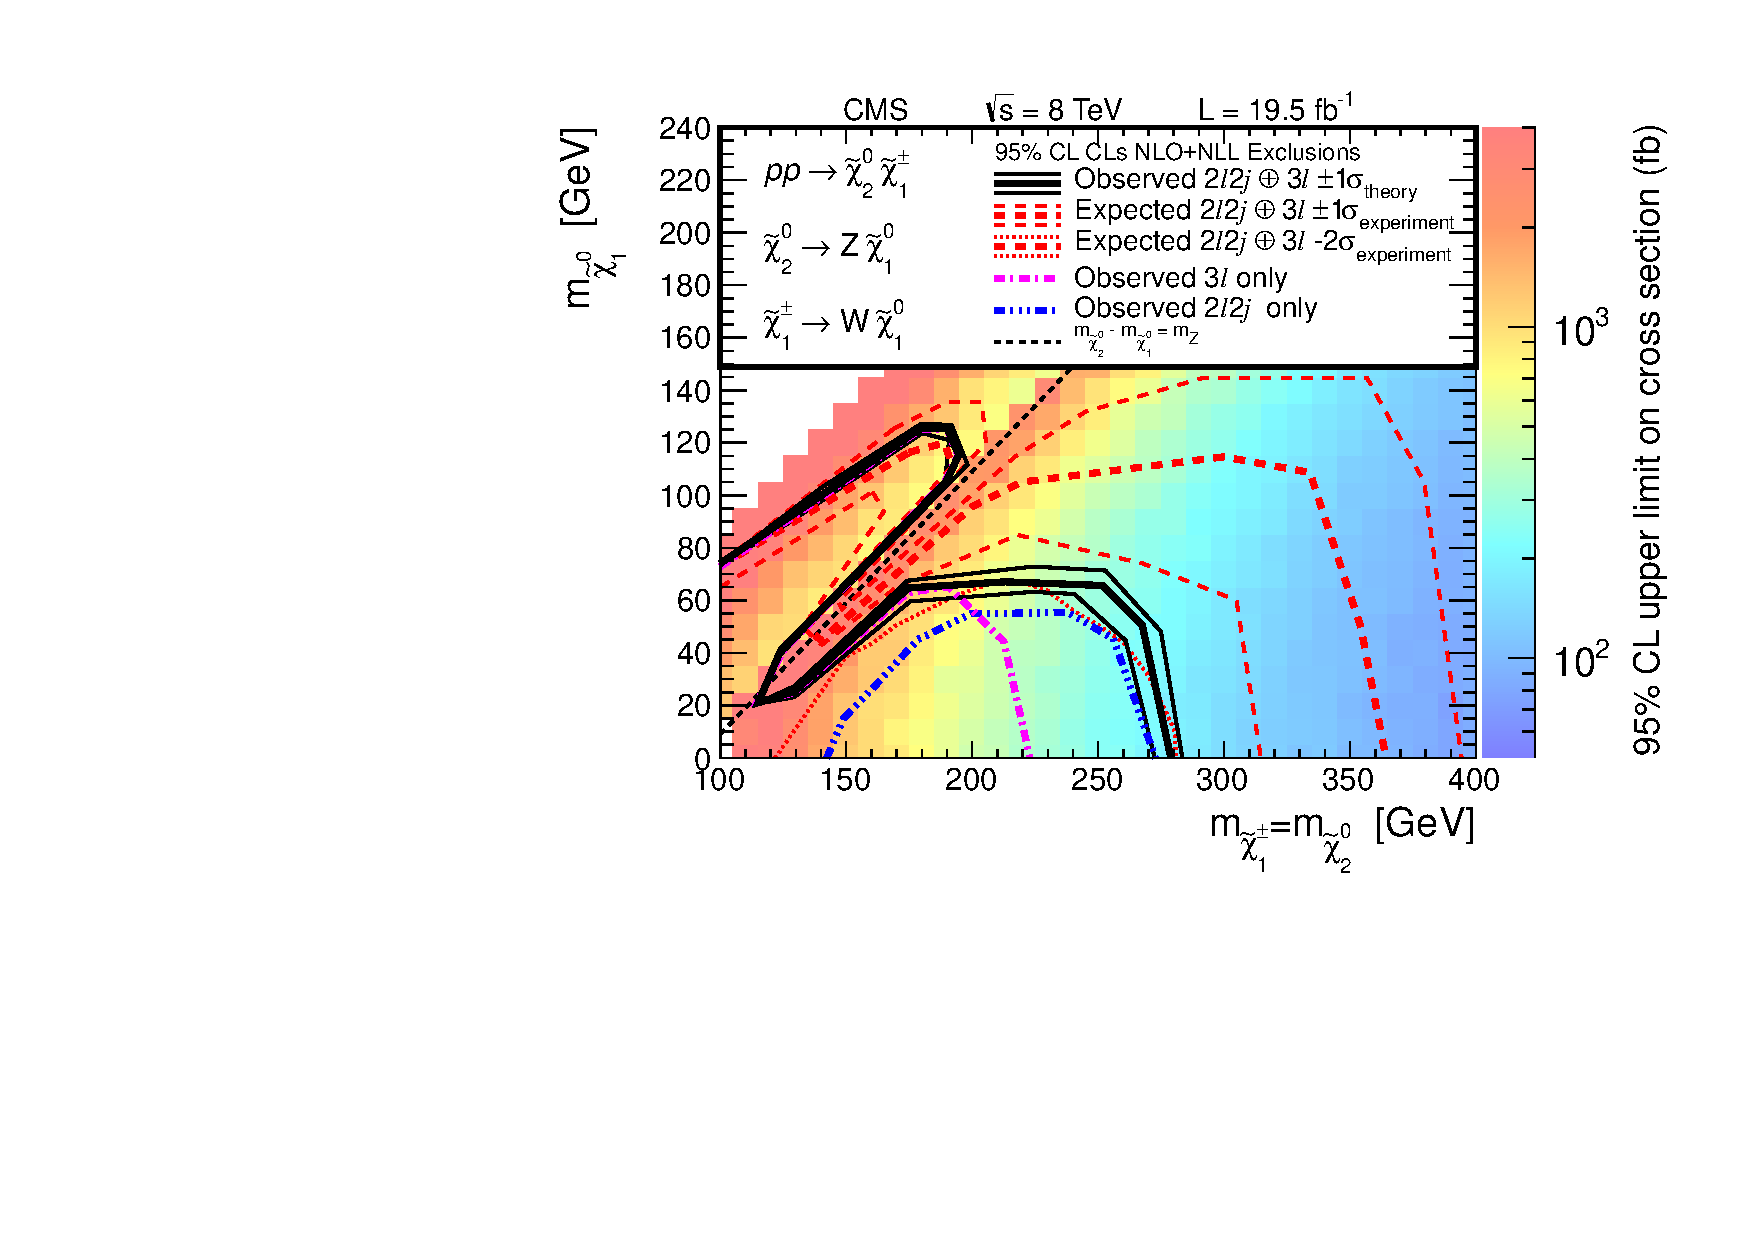
\includegraphics[width=\textwidth]{figures/interpretations/TChiWZ_previous_best.pdf}
          \caption{Previous best limits on this model}
        \end{subfigure}
        \begin{subfigure}[b]{0.4\textwidth}
          \label{fig:t5zz_interpretations_current}
          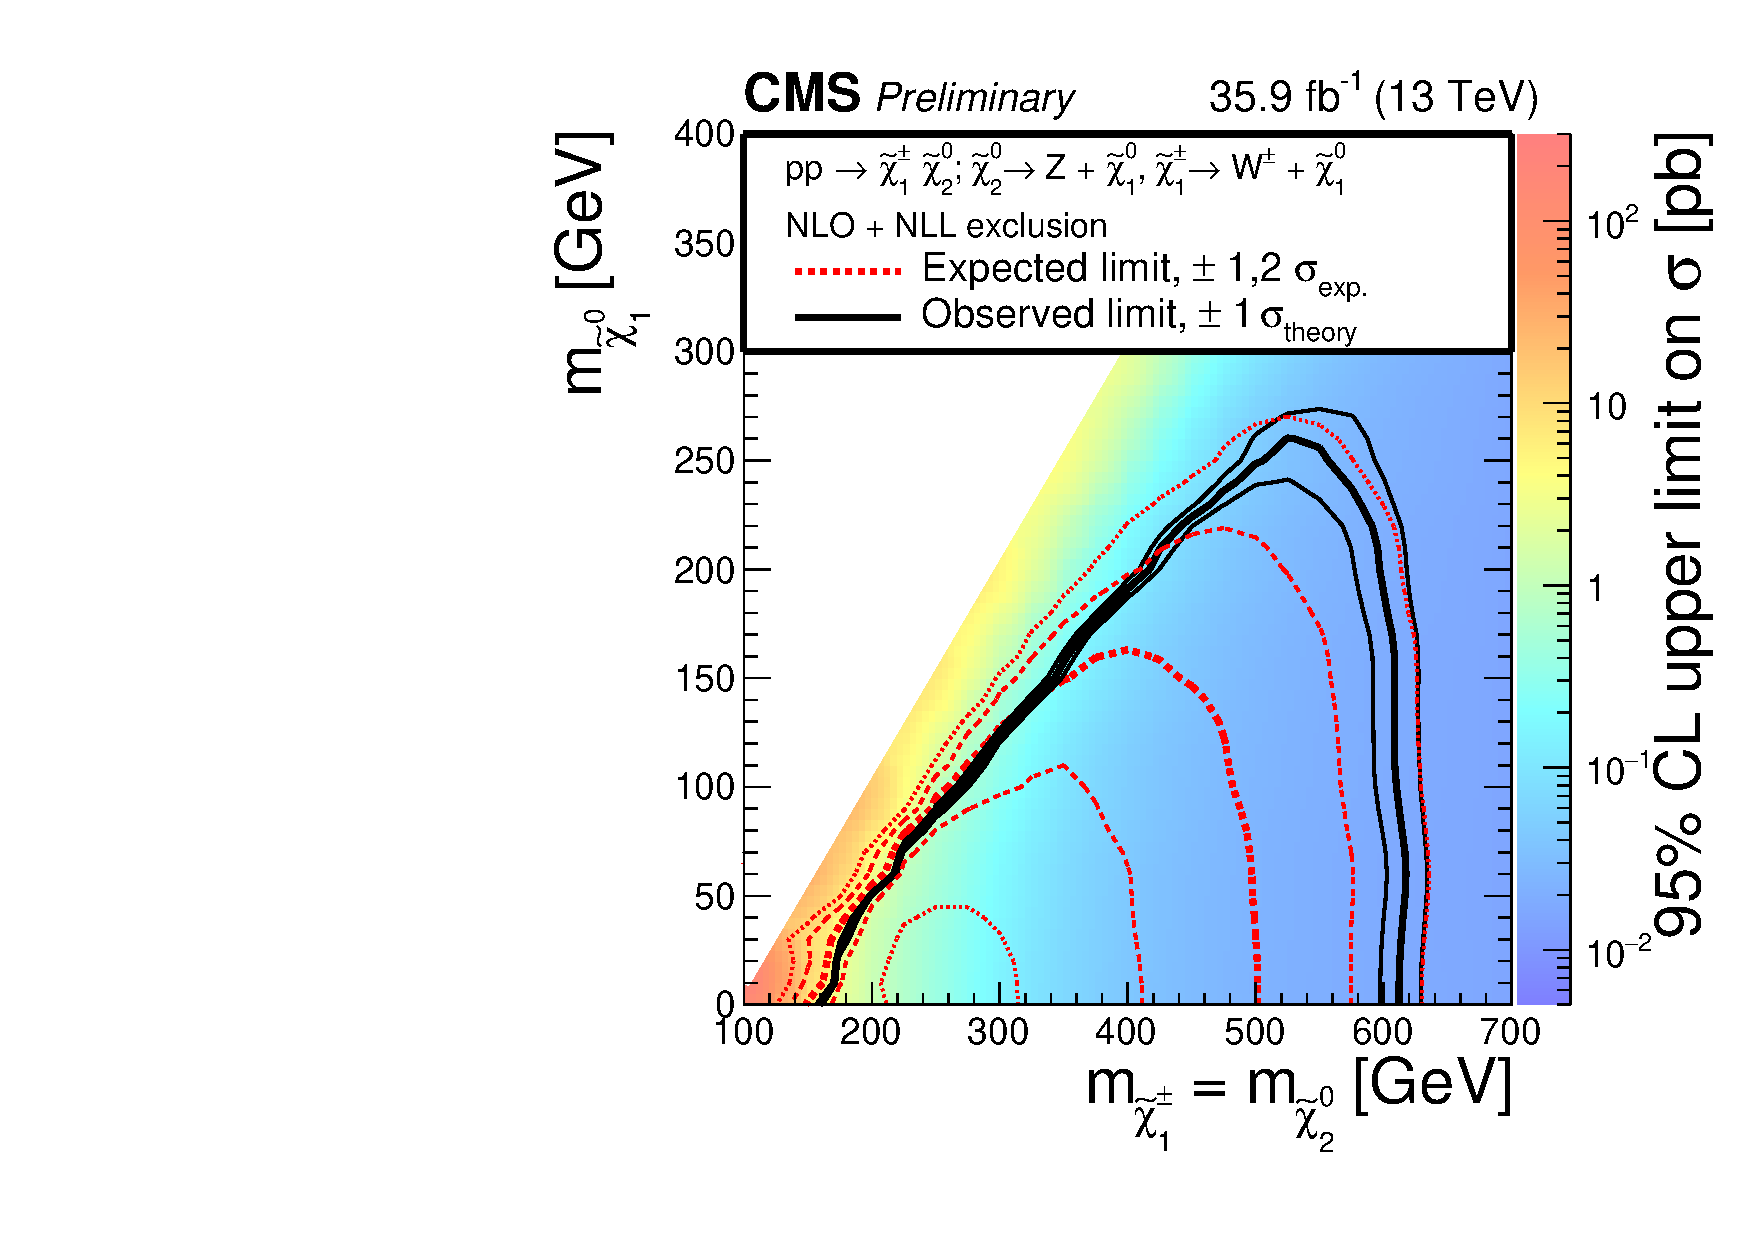
\includegraphics[width=\textwidth]{figures/interpretations/TChiWZ_Exclusion_13TeV.pdf}
          \caption{Limits set by this analysis}
        \end{subfigure}
      \caption[The limits set on the electroweak WZ model.]{ \label{fig:tchiwz_interpretation}
        The limits set on the electroweak WZ model in fig. \ref{fig:tchiwz_diagram_interpretations}. In this limit, data from the electroweak VZ and HZ search regions are utilized, though the VZ region has by far the larger sensitivity to this model. The solid back and thick dashed red lines show the observed and expected limits respectively as described in section \ref{sec:setting_exclusion_limits}, mass points below these lines are excluded. These results push the excluded $\widetilde{\chi}^{\pm}_1$ and $\widetilde{\chi}^0_2$ masses to 600 GeV from 275 GeV for low mass LSPs, and excludes LSP mass points for up to about 250 GeV for high $\widetilde{\chi}^{\pm}_1$ and $\widetilde{\chi}^0_2$ masses, up from about 60.
      }
    \end{figure}

    Figure \ref{fig:tchizz_interpretation}, shows the exclusion limits for the electroweak ZZ model shown in fig. \ref{fig:tchizz_diagram_interpretations}. In this model, the only free parameter is the mass of the $\widetilde{\chi}^0_1$, the gravitino mass is assumed to be 1 GeV. The thick pink line is the theoretical cross section for this model as a function of the free mass parameter, its thickness shows the uncertainty on the theory calculation. The solid black and dotted black lines show the observed and expected limits respectively. The point where the pink line and the solid black line cross is the observed exclusion limit for the $\widetilde{\chi}^0_1$ mass at 95\% confidence. This result pushed the previous limits on the $\widetilde{\chi}^0_1$ mass from about 375 GeV to about 675 GeV.


    \begin{figure}[!h]
      \centering
        \begin{subfigure}[b]{0.4\textwidth}
          \label{fig:t5zz_interpretations_2015}
          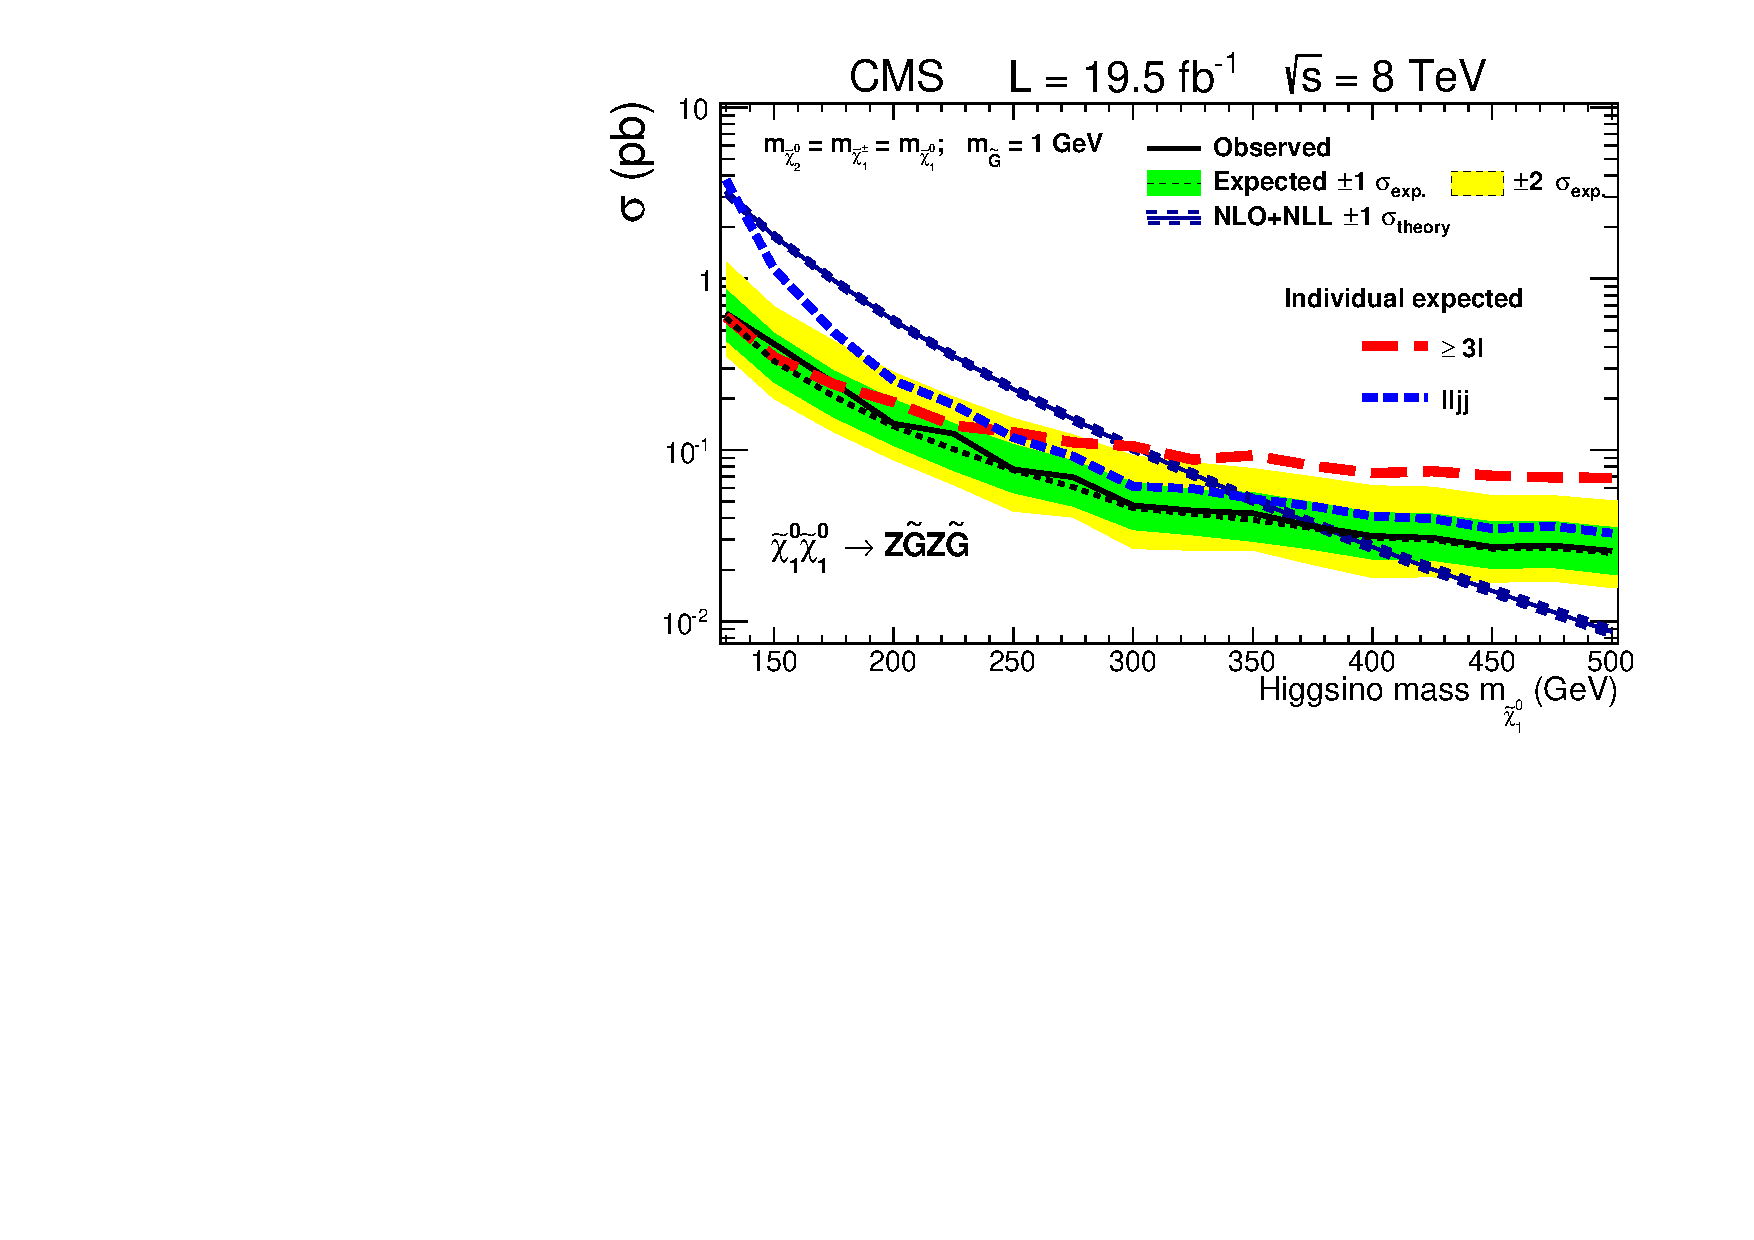
\includegraphics[width=\textwidth]{figures/interpretations/TChiZZ_previous_best.pdf}
          \caption{Previous best limits on this model}
        \end{subfigure}
        \begin{subfigure}[b]{0.4\textwidth}
          \label{fig:t5zz_interpretations_current}
          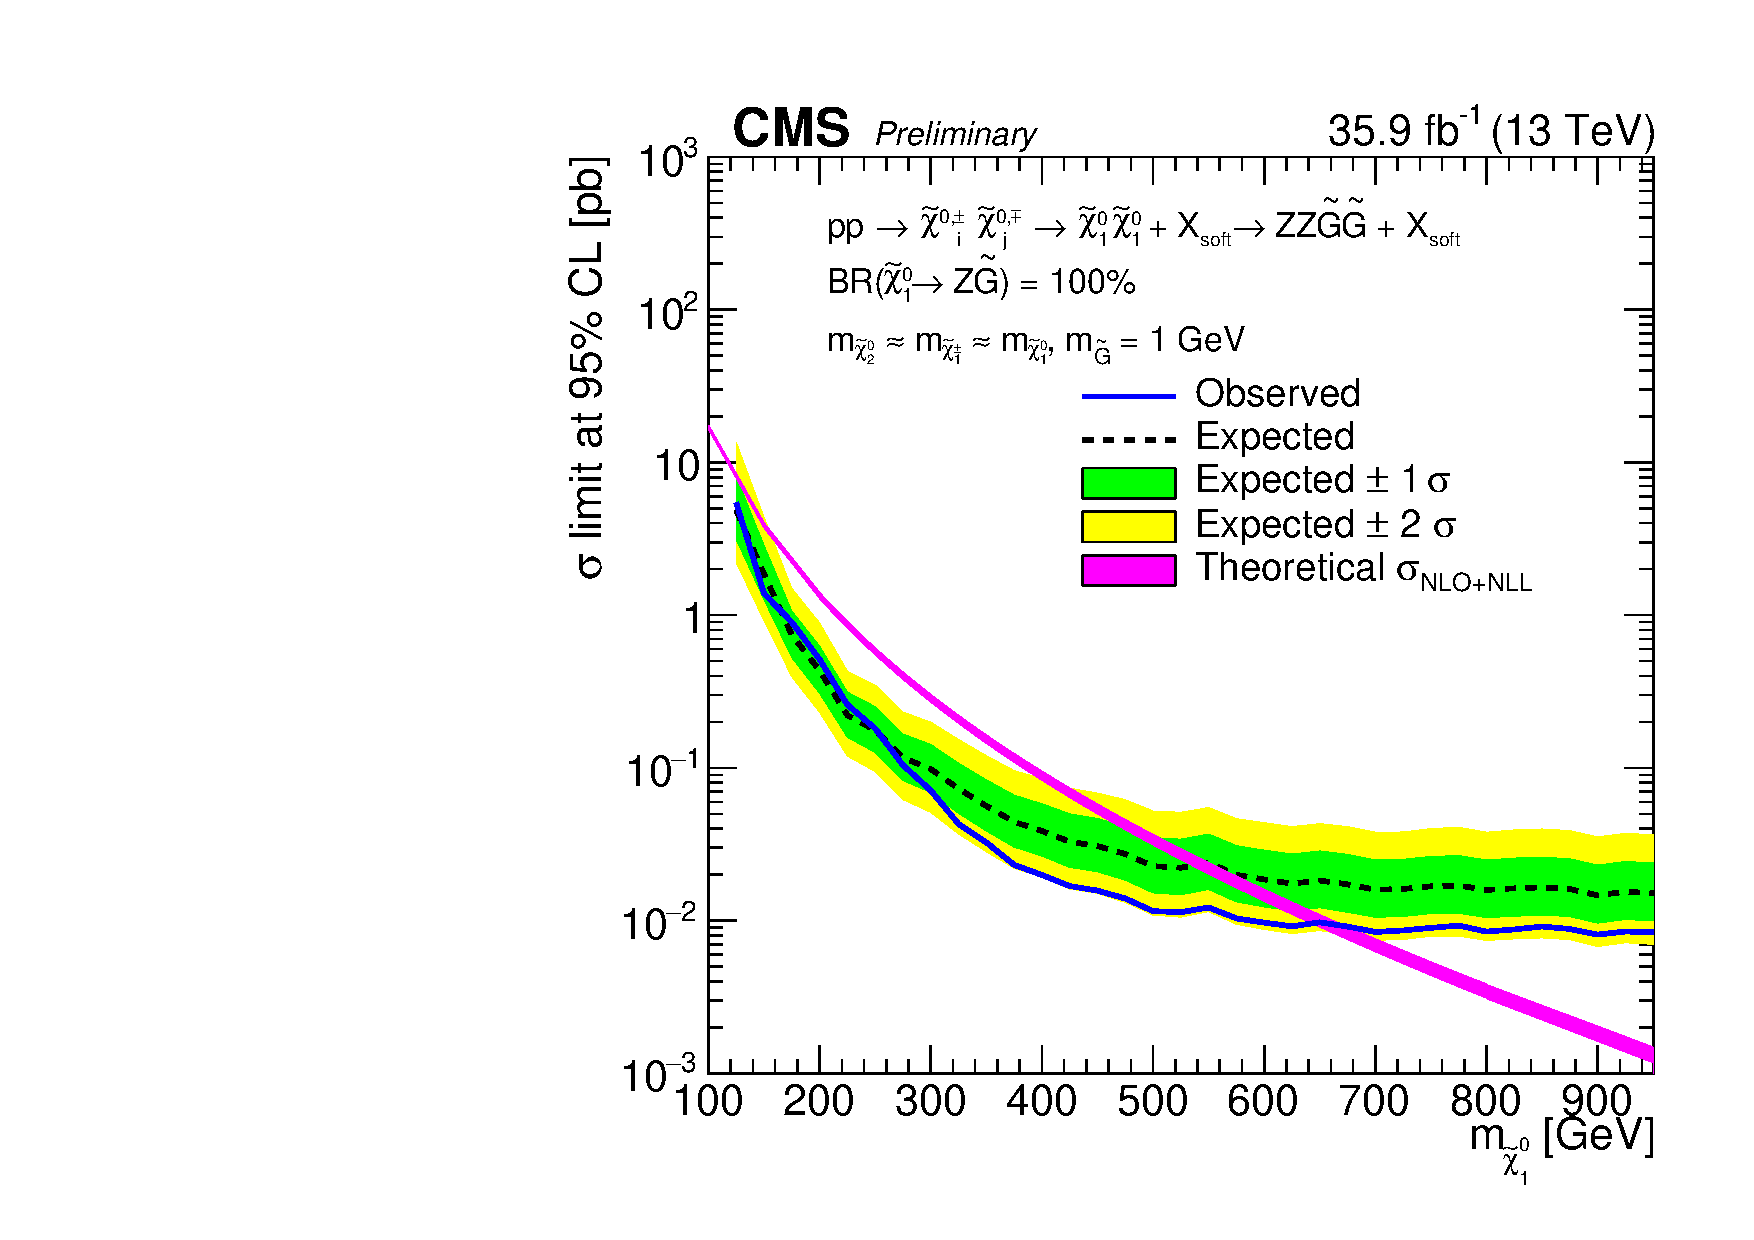
\includegraphics[width=\textwidth]{figures/interpretations/TChiZZ_Exclusion_13TeV.pdf}
          \caption{Limits set by this analysis}
        \end{subfigure}
      \caption[The limits set on the Electroweak ZZ model.]{ \label{fig:tchizz_interpretation}
        The limits set on the Electroweak ZZ model shown in fig. \ref{fig:tchizz_diagram_interpretations}. In this limit, data from the electroweak VZ search region is utilized and the $\widetilde{\chi}^0_1$ is assumed to decay 100\% to the Z. On the right, the point where the pink line crosses the solid black line marks the highest mass excluded. Where the pink line crosses the dotted line marks the expected limit. The downward fluctuation in the VZ region high \MET bin again caused the observed limit to be better than the expected limit. The limit set on the $\widetilde{\chi}^0_1$ mass increased by about 300 GeV from the previous result on the left.
      }
    \end{figure}

    Finally, figure \ref{fig:tchihz_interpretation}, shows the exclusion limits for the electroweak HZ model shown in fig. \ref{fig:tchihz_diagram_interpretations}. The only free parameter in this model is the $\widetilde{\chi}^0_1$ mass. This model assumes a 50\% branching ratio of the $\widetilde{\chi}^0_1$ to higgs and Z bosons. The likelihood for this model is constructed using data from the VZ and HZ regions. The likelihood also takes into account that the signature of the ZZ model above should be produced with $\frac{1}{2}$ the frequency as that of the HZ model since the 50\% branching ratio to Z bosons means that the ZZ final state should be produced as well. Points to the left of the crossing point between the pink and solid black line are excluded at the 95\% level. This analysis pushed the limits for the $\widetilde{\chi}^0_1$ mass in this model from 250 GeV to about 500 GeV.

    \begin{figure}[!h]
      \centering
        \begin{subfigure}[b]{0.4\textwidth}
          \label{fig:t5zz_interpretations_2015}
          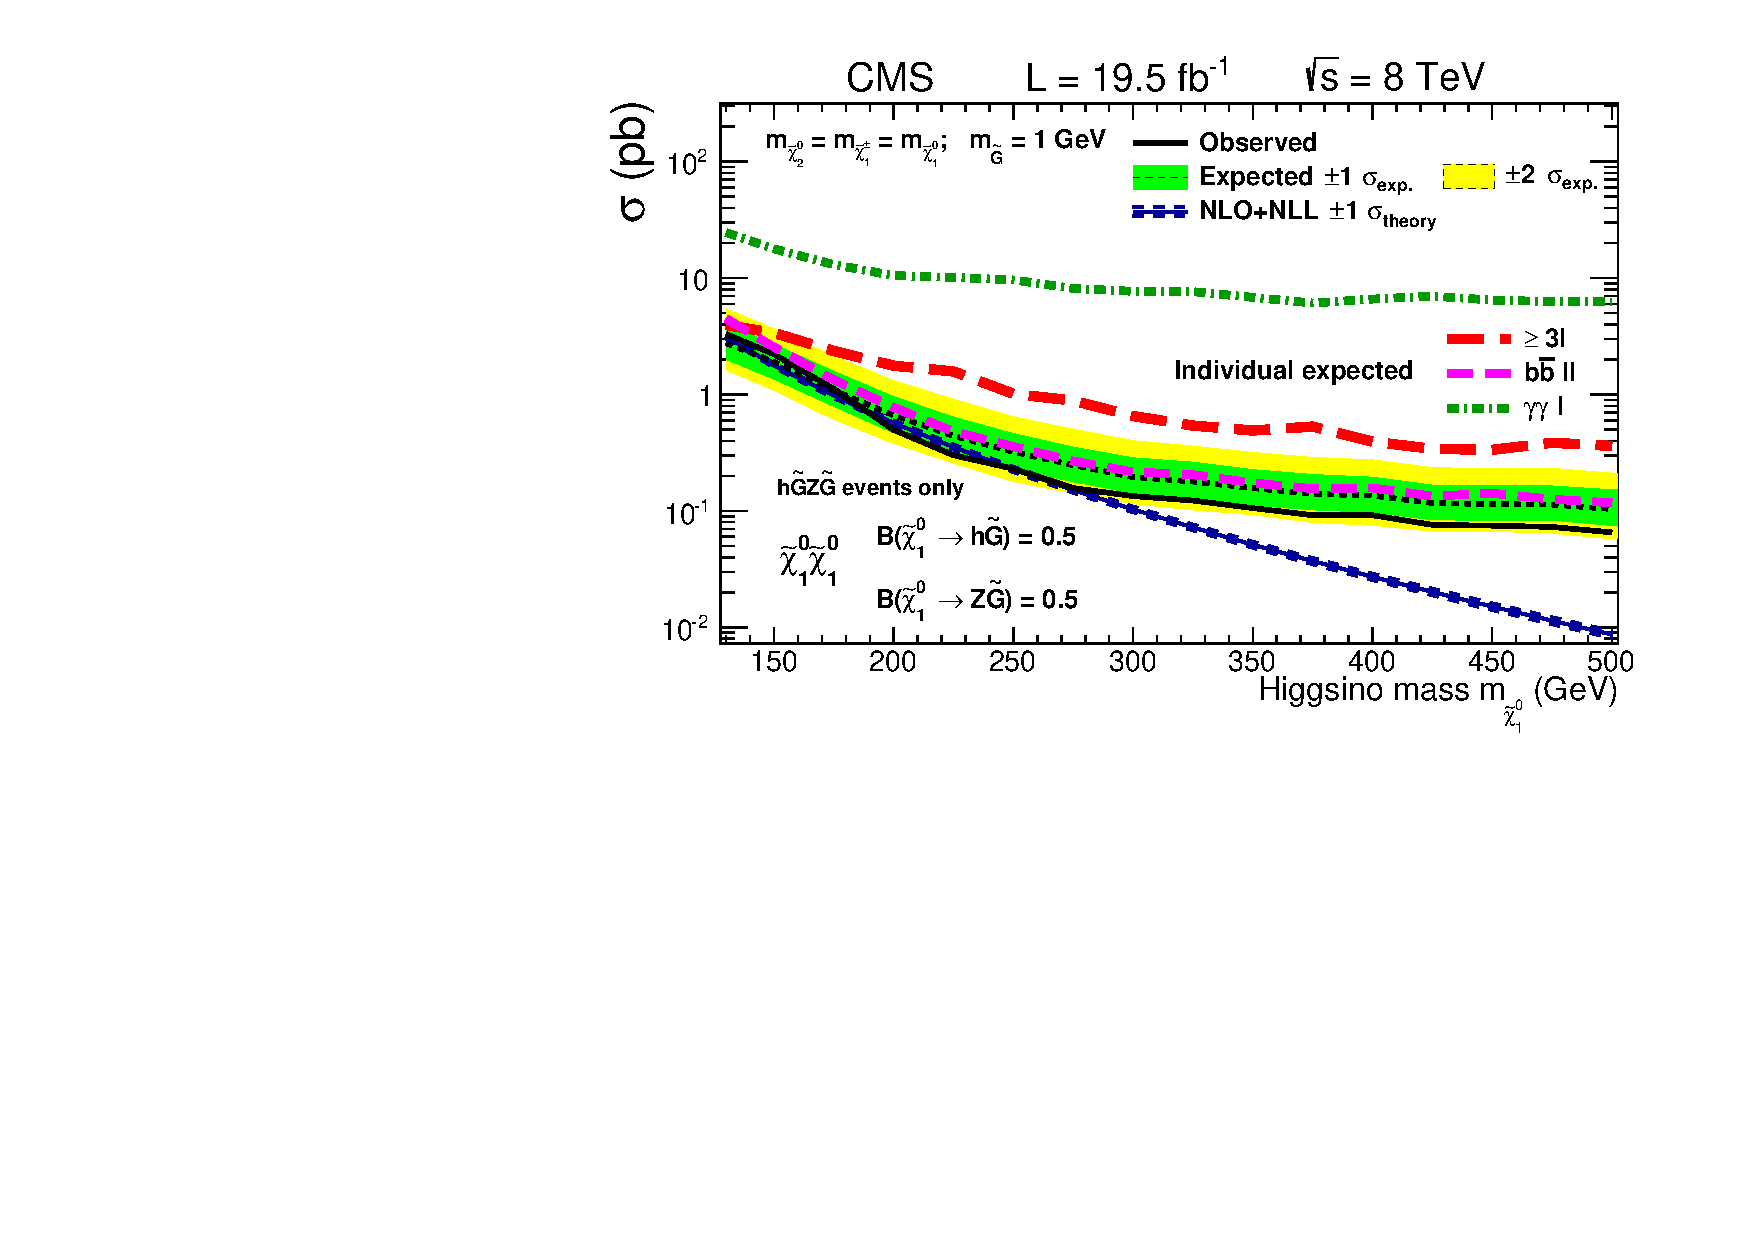
\includegraphics[width=\textwidth]{figures/interpretations/TChiHZ_previous_best.pdf}
          \caption{Previous best limits on this model}
        \end{subfigure}
        \begin{subfigure}[b]{0.4\textwidth}
          \label{fig:t5zz_interpretations_current}
          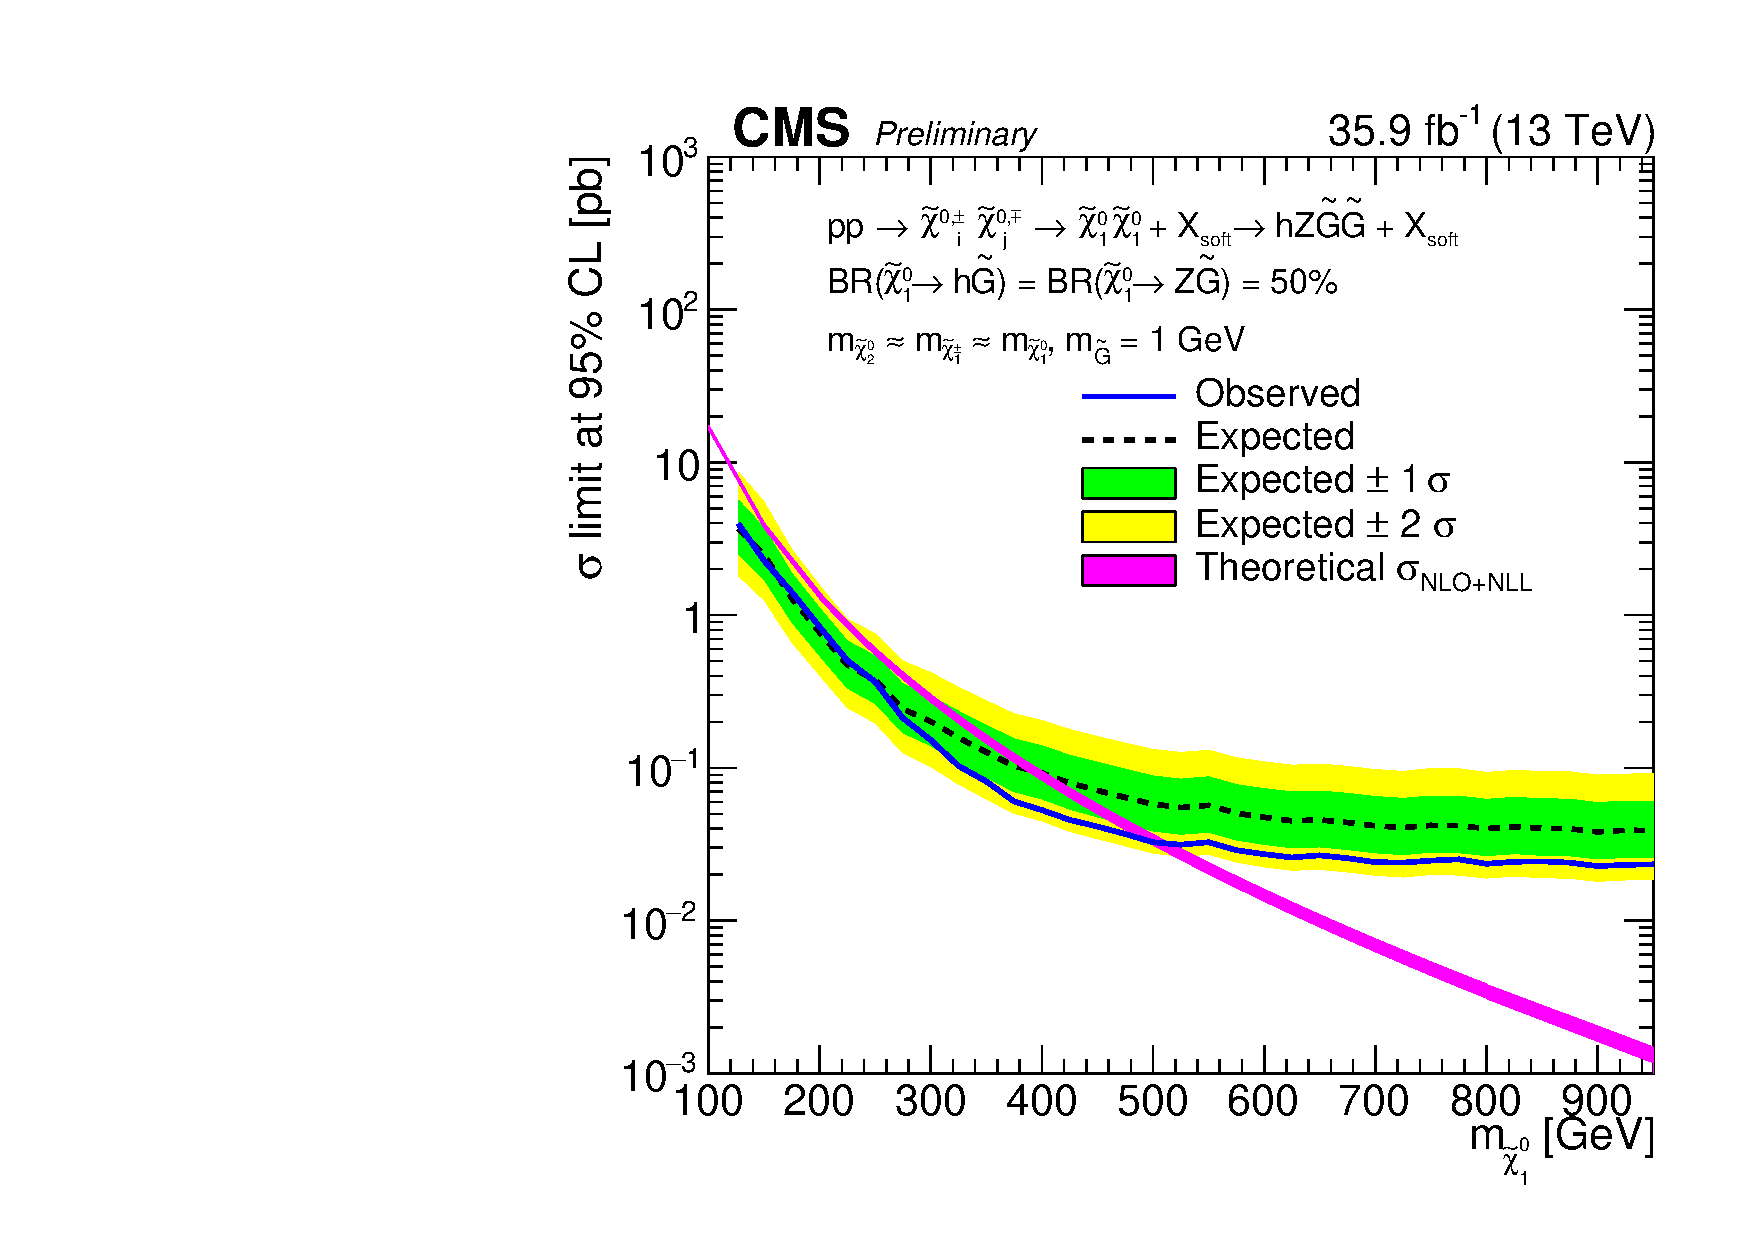
\includegraphics[width=\textwidth]{figures/interpretations/TChiHZ_0p25ZZ_Exclusion_13TeV.pdf}
          \caption{Limits set by this analysis}
        \end{subfigure}
      \caption[The limits set on the Electroweak HZ model.]{ \label{fig:tchihz_interpretation}
        The limits set on the Electroweak HZ model shown in fig. \ref{fig:tchihz_diagram_interpretations}. In this limit, data from the electroweak VZ and HZ search regions are combined and the branching ratios for $\widetilde{\chi}^0_1$ are assumed to be 50/50 between the Higgs and Z.
      }
    \end{figure}

  \clearpage
  \section{Acknowledgments}

  In the previous chapter, I presented a search for new physics which relied heavily on the work of several collaborators. This work would have been impossible without the leadership of Dominick Olivito, Pablo Martinez Ruiz del Arbol, and Vince Welke. In addition, the analysis relied on direct contributions from Christian Schomakers, Leonora Vesterbacka, and Sergio Sánchez Cruz. I would also like to thank CMS members (and my co-chairs) Frank W\"uerthwein and Avraham Yagil for their mentorship and support, their group has developed this search over many years. In addition to my direct collaborators, the CMS collaboration itself consists of over 4000 members who built the infrastructure to acquire data, provided crucial feedback and internal review of analysis methodology, and supplied indispensable tools for this analysis, e.g. the b-tagging software suite and the MVA for electron identification. I would like to acknowledge all members of CMS, past and present, for their tremendous contributions to this work, enabling a few people with laptops to search for new fundamental particles.

  I must also specifically thank my co-authors on CMS for contributing figure \ref{fig:t5zz_interpretation} (a), showing the previous best limits on the strong GMSB SUSY model.
%\section{The Electroweak Combination}

%The things we want to consider here are: 

%  1. All the cuts and stuff, I want to list out what cuts we made and why we chose them. I am not sure where I will put all the data/MC agreement stuff. I guess that's mostly important for the MET profile as I don't really use MC in the rest of the
